\documentclass{article}
\newcommand{\ourdata}{OurData}
\usepackage[utf8]{inputenc}
\usepackage{svg}
\usepackage[utf8]{inputenc}
\usepackage{pgfplots}
\pgfplotsset{compat=1.18}
\usepackage{tikz}
\usepackage{float}
\usepackage{enumitem}
\usepackage{makecell}
\newcommand{\ourmodel}{OurModel}
% if you need to pass options to natbib, use, e.g.:
%     \PassOptionsToPackage{numbers, compress}{natbib}
% before loading neurips_2026

% The authors should use one of these tracks.
% Before accepting by the NeurIPS conference, select one of the options below.
% 0. "default" for submission
\usepackage[preprint]{neurips_2026}
\newcommand{\ourmethod}{OurMethod}
% the "default" option is equal to the "main" option, which is used for the Main Track with double-blind reviewing.
% 1. "main" option is used for the Main Track
%  \usepackage[main]{neurips_2026}
% 2. "position" option is used for the Position Paper Track
%  \usepackage[position]{neurips_2026}
% 3. "eandd" option is used for the Evaluations & Datasets Track
 % \usepackage[eandd]{neurips_2026}
 % if you need to opt-in for a single-blind submission in the E&D track:
 %\usepackage[eandd, nonanonymous]{neurips_2026}
% 4. "creativeai" option is used for the Creative AI Track
%  \usepackage[creativeai]{neurips_2026}
% 5. "sglblindworkshop" option is used for the Workshop with single-blind reviewing
 % \usepackage[sglblindworkshop]{neurips_2026}
% 6. "dblblindworkshop" option is used for the Workshop with double-blind reviewing
%  \usepackage[dblblindworkshop]{neurips_2026}

% After being accepted, the authors should add "final" behind the track to compile a camera-ready version.
% 1. Main Track
 % \usepackage[main, final]{neurips_2026}
% 2. Position Paper Track
%  \usepackage[position, final]{neurips_2026}
% 3. Evaluations & Datasets Track
 % \usepackage[eandd, final]{neurips_2026}
% 4. Creative AI Track
%  \usepackage[creativeai, final]{neurips_2026}
% 5. Workshop with single-blind reviewing
%  \usepackage[sglblindworkshop, final]{neurips_2026}
% 6. Workshop with double-blind reviewing
%  \usepackage[dblblindworkshop, final]{neurips_2026}
% Note. For the workshop paper template, both \title{} and \workshoptitle{} are required, with the former indicating the paper title shown in the title and the latter indicating the workshop title displayed in the footnote.
% For workshops (5., 6.), the authors should add the name of the workshop, "\workshoptitle" command is used to set the workshop title.
% \workshoptitle{WORKSHOP TITLE}

% "preprint" option is used for arXiv or other preprint submissions
 % \usepackage[preprint]{neurips_2026}

% to avoid loading the natbib package, add option nonatbib:
%    \usepackage[nonatbib]{neurips_2026}

\usepackage[utf8]{inputenc} % allow utf-8 input
\usepackage[T1]{fontenc}    % use 8-bit T1 fonts
\usepackage{hyperref}       % hyperlinks
\usepackage{url}            % simple URL typesetting
\usepackage{booktabs}       % professional-quality tables
\usepackage{amsfonts}       % blackboard math symbols
\usepackage{nicefrac}       % compact symbols for 1/2, etc.
\usepackage{microtype}      % microtypography
\usepackage{xcolor}         % colors
\usepackage{graphicx}
\usepackage{amssymb} 
\usepackage{amsmath}
\usepackage{booktabs}
\usepackage{array}
\usepackage{enumitem}
\usepackage{algorithm}
\usepackage{wrapfig}
\usepackage{caption}
\usepackage{algpseudocode} % ← 推荐（比 algorithmic 更现代）
\usepackage{xcolor}
\usepackage{tabularx}
\usepackage{tcolorbox}
\usepackage{fontawesome5}
\usepackage{booktabs}
\usepackage{multirow}
\usepackage{wrapfig}
\usepackage{colortbl} 

\definecolor{mintbg}{RGB}{220, 245, 230}
\definecolor{headerblue}{RGB}{220,235,250}
\definecolor{zebrablue}{RGB}{235, 243, 252}
\usepackage[scaled]{inconsolata}

% Color palette (matches the chart's outer ring)
\definecolor{musicTint}{HTML}{92B4C8}     % Music = light blue
\definecolor{textTint}{HTML}{EEA599}      % Text  = coral
\definecolor{speechTint}{HTML}{FAC795}    % Speech = orange
\definecolor{soundTint}{HTML}{ABD3E1}     % Sound = pale aqua

% Substantial colored band of CONSTANT width (centered in its half-row).
% Adjust \bandwidth to taste — 3.0cm = narrower, 4.0cm = wider.
\setlength{\fboxsep}{0pt}
\newlength{\bandwidth}
\setlength{\bandwidth}{5.0cm}
\newcommand{\bannerL}[2]{%
  \multicolumn{2}{@{}l@{}}{%
    \colorbox{#1}{\strut\makebox[\bandwidth][l]{~\textbf{\textit{#2}}}}}}
\newcommand{\bannerR}[2]{%
  \multicolumn{2}{@{}l@{}}{%
    \colorbox{#1}{\strut\makebox[\bandwidth][l]{~\textbf{\textit{#2}}}}}}
      
\usepackage{multirow}
\usepackage{array}
\usepackage[table]{xcolor}
\usepackage{subcaption}
\usepackage{graphicx}
\usepackage{caption}
\usepackage{pifont}
\captionsetup[sub]{font=footnotesize,skip=3pt}
\newcommand{\best}[1]{\textbf{#1}}

\newcommand{\tcpblue}[1]{\textcolor{blue}{\hfill //~#1}}
\newcommand{\halfchunk}{\frac{1}{2}\mathrm{chunk}}
\usepackage[normalem]{ulem}



\usepackage{makecell}

% Note. For the workshop paper template, both \title{} and \workshoptitle{} are required, with the former indicating the paper title shown in the title and the latter indicating the workshop title displayed in the footnote. 
\title{Audio Interaction Model }


% The \author macro works with any number of authors. There are two commands
% used to separate the names and addresses of multiple authors: \And and \AND.
%
% Using \And between authors leaves it to LaTeX to determine where to break the
% lines. Using \AND forces a line break at that point. So, if LaTeX puts 3 of 4
% authors names on the first line, and the last on the second line, try using
% \AND instead of \And before the third author name.

\author{%
  Zhifei Xie\textsuperscript{1*} \quad Zihang Liu\textsuperscript{2*} \quad Ze An\textsuperscript{2} \quad \textbf{Xiaobin Hu}\textsuperscript{2}\quad \textbf{Yue Liao}\textsuperscript{2} \\ \textbf{Ziyang Ma}\textsuperscript{1}\quad \textbf{Dongchao Yang}\textsuperscript{3} \quad \textbf{Mingbao Lin}\textsuperscript{2$\dagger$} \quad \textbf{Deheng Ye}\textsuperscript{1$\dagger$}\\ \textbf{Shuicheng Yan}\textsuperscript{2$\dagger$} \quad \textbf{Chunyan Miao}\textsuperscript{1$\dagger$}\\
  \textsuperscript{1}NTU \quad \textsuperscript{2}NUS \quad \textsuperscript{3}CUHK\\
  \faEnvelope~\href{mailto:Zhifei001@e.ntu.edu.sg}{\texttt{Zhifei001@e.ntu.edu.sg}}%
}

\begin{document}

\maketitle

\vspace{-7mm}

\newcommand{\logoblog}{\raisebox{-0.2ex}{
\includegraphics[height=1em]{fig/logo.png}}}
\newcommand{\logohf}{\raisebox{-0.2ex}{
\includegraphics[height=1em]{fig/huggingface.png}}}
\newcommand{\logogh}{\raisebox{-0.2ex}{
\includegraphics[height=1em]{fig/github.png}}}
\definecolor{deepblue}{RGB}{0, 45, 114}
\definecolor{promptbg}{RGB}{221, 235, 247}
\definecolor{promptframe}{RGB}{91, 155, 213}


\vspace{-2mm}
\begin{center}
\begin{minipage}{0.7\textwidth}
\logoblog~\textbf{Project page:} \href{https://xzf-thu.github.io/Audio-Interaction}{\texttt{\textcolor{deepblue}{https://xzf-thu.github.io/Audio-Interaction}}} \\
\logohf~\textbf{Data:} \href{https://huggingface.co/datasets/zhifeixie/StreamAudio-2M}{\texttt{\textcolor{deepblue}{huggingface.co/datasets/zhifeixie/StreamAudio-2M}}} \\
\end{minipage}
\end{center}
\vspace{-2mm}


\begin{abstract}
Audio is an inherently interactive modality, yet today's Large Audio Language Models (LALMs) are offline, and streaming audio models each handle only a single task such as streaming ASR or voice chatting. It is time to unify them into one online LALM: a model that, through an always-on \underline{\emph{perceive--decide--respond}} loop, listens to sound, environment, and instructions in real time and reacts on the fly. We formalize this regime as the \underline{\textbf{\textsc{Audio Interaction Model}}}, and realize it with \textbf{\textsc{Audio-Interaction}}, a unified streaming model that retains offline task execution while adding online general audio instruction following, from dialogue to full voice chatting, deciding when to respond from the semantics of the stream. To enable this, we propose \textbf{\textsc{SoundFlow}}, a framework that instantiates the perceive--decide--respond loop end to end, from data to training to deployment, through streaming-native data construction, comprehension-aware training, and asynchronous low-latency inference for stable real-time interaction. We further construct \textbf{\textsc{StreamAudio-2M}}, a 2.6M-item streaming corpus spanning 7 fundamental abilities and 28 sub-tasks, and \textbf{\textsc{Proactive-Sound-Bench}} for evaluating proactive audio intervention. Across 8 benchmarks, Audio-Interaction preserves competitive performance on mainstream audio tasks while unlocking capabilities inaccessible to offline LALMs, including real-time ASR, streaming audio instruction following, and proactive help.
\end{abstract}

% \textsc{Audio-Interaction} listens to a continuous audio stream and decides at each moment whether to stay silent or speak, unifying conventional capabilities (e.g., dialogue, ASR) and streaming-native capabilities (e.g., simultaneous translation, proactive intervention) within a single model.

\begin{figure*}[!h]
\centering
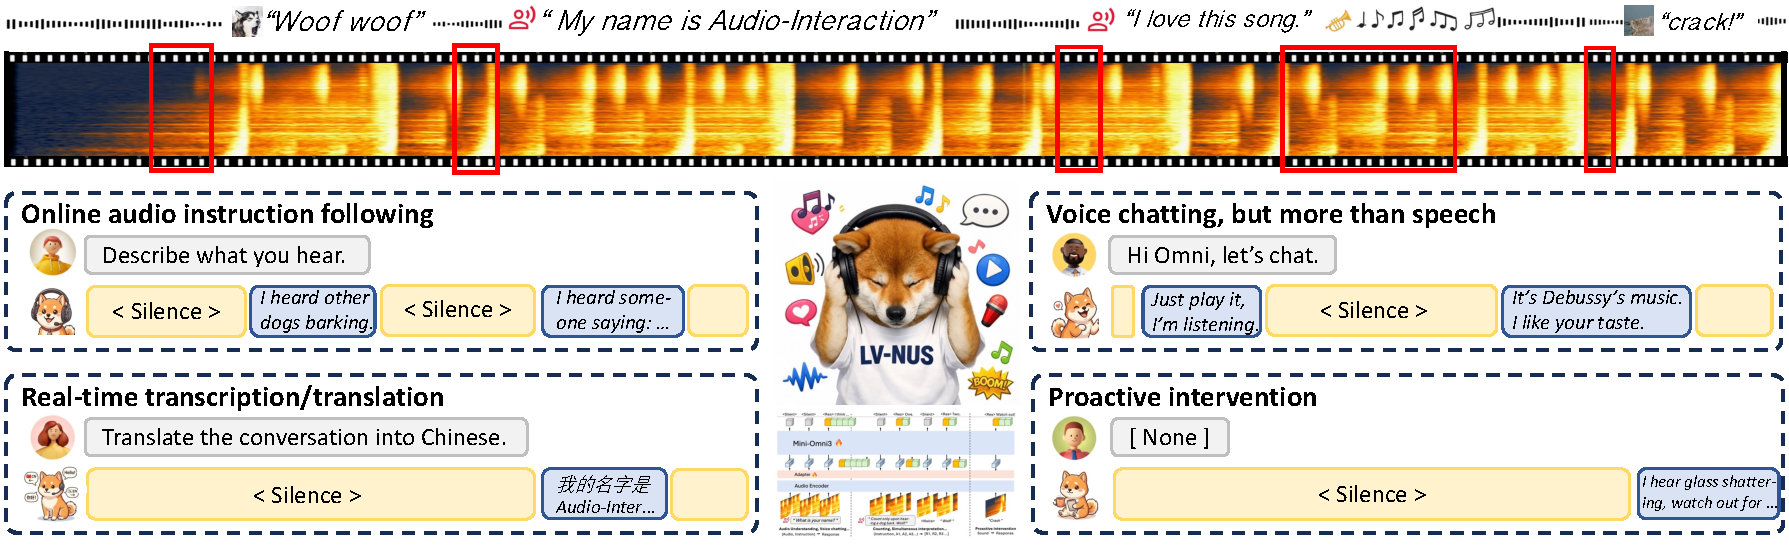
\includegraphics[width=\linewidth]{fig/figure1-overview-newname.pdf}
\caption{\textsc{Audio-Interaction} listens to a continuous audio stream and decides at each moment whether to stay silent or speak, unifying conventional capabilities (e.g., dialogue, ASR) and streaming-native (e.g., simultaneous translation, proactive help) capabilitie within a single model.}
\label{figure1-overview}
\end{figure*}

\vspace{-2mm}
\section{Introduction}

Audio is an inherently real-time and interactive modality at its core. Unlike text, which compresses events into symbolic form, or images, which capture static snapshots, audio is a continuous, always-on channel through which humans perceive and respond to their surroundings. Alongside rapid advances in large language models~\citep{brown2020language, touvron2023llama, achiam2023gpt}, reinforcement learning~\citep{ouyang2022training, rafailov2023direct}, and agentic intelligence~\citep{yao2022react, schick2023toolformer}, large audio language models (LALMs) have undergone a comparable transformation~\citep{chu2023qwen, tang2023salmonn, chu2024qwen2, xie2024mini}, performing fine-grained emotion recognition, multi-step reasoning, tool use, and even code generation directly from acoustic inputs. Together, these advances move audio from narrow recognition tasks toward general-purpose intelligence.

\vspace{1mm}
However, current LALMs still follow the conventional offline input-output formulation $y = f(x, A)$, mirroring multimodal designs such as LLaVA~\citep{llava}, which poorly matches the real-time and interactive nature of audio. \textbf{A common bridge has been to train a dedicated streaming model for each important task}, e.g., dialogue~\citep{defossez2024moshi, fang2024llama, xie2024mini} and streaming speech recognition~\citep{gao2022paramformer}, but this bridging approach has two fundamental problems: \underline{\textit{(i) every}} \underline{\textit{capability requires its own model trained from scratch}}, and \underline{\textit{(ii) each model handles only a narrow}} \underline{\textit{capability}}. For instance, even fully-streaming systems such as Moshi~\citep{defossez2024moshi}, despite strong conversational capability, cannot interpret a hesitant pause or recognize a cough. \textbf{So, it is time to move toward a new paradigm beyond LALMs: Large Audio Interaction Models (LAIMs)}, an all-in-one framework that subsumes existing tasks within a single interactive model and bridges the gap between LALM-level capabilities and the real-time nature of audio.

\vspace{1mm}
Moving to this regime surfaces two fundamental challenges absent from its offline predecessor.
%
\textbf{(C1) Comprehension-grounded response triggering.}
Offline LALMs respond passively to a fully observed clip, whereas an interactive model must decide \emph{whether to respond} at every chunk based on semantic understanding of the unfolding context, not surface-level acoustic cues. Supervision for this decision is sparse and temporally ambiguous, and no existing corpus pairs continuous audio with properly timed intervention cues, requiring large-scale audio stitching for training data construction.
%
\textbf{(C2) Real-time context continuity under chunked inference.}
Audio must be consumed in fixed-length chunks to meet low-latency requirements, but chunking breaks the temporal continuity of acoustic signals and the long-range context accumulated across the interaction. The model must reconstruct continuity across chunks and retain earlier context without inflating the inference window or stalling on encoder-decoder synchronization. 


\vspace{1mm}
\underline{\textit{We instantiate this regime as \textbf{\textsc{Audio-Interaction}}, an always-on audio interaction model}} train- ed within our \textbf{\textsc{SoundFlow}} framework. \textsc{Audio-Interaction} consumes audio one chunk at a time and, at each step, makes a comprehension-grounded decision between responding and remaining silent, forming a always-on \emph{perceive--decide--respond} loop. Under this loop, traditional audio capabilities such as translation, recognition, and dialogue are naturally unified as instructions within a single interactive paradigm. \textbf{\textsc{SoundFlow} is an end-to-end audio-based interaction framework spanning data, training, and inference, with three components:} \textbf{i)} \emph{interaction data synthesis} via a hierarchical event curation pipeline that composes short clips into coherent long-form interactions, with a time-frequency joint preprocessing module (\textsc{TFJP}) that smooths boundaries and suppresses noise to mimic real-world recordings; \textbf{ii)} \emph{interaction-aware training} that casts audio modeling as chunk-level sequential decision, with history review and comprehension-aware silence addressing context forgetting and false triggering; \textbf{iii)} \emph{asynchronous interactive inference} whose first-in-first-out scheme decouples encoding from decoding, eliminating stalling and cutting first-frame latency by $4.5\times$. \underline{\textit{Feeding this framework is \textbf{\textsc{StreamAudio-2M}}}}, a \textbf{302k-hour}, \textbf{2.6M-item} corpus spanning \textbf{28} interactive sub-tasks across \textbf{7} major categories, where each sample is a $3$-$15$ turn interaction with sparse, context-dependent response cues. We further release \underline{\textit{\textbf{\textsc{ProactiveSound-Bench}}}} to evaluate a new capability, audio-based proactive assistance, which contains \textbf{644} \textit{human-designed} events that probe whether a model can proactively interupt with no instruction. 

\vspace{1mm}
\textbf{We empirically validate \textsc{Audio-Interaction} from two perspectives.} First, from a performance standpoint, we demonstrate that converting the model from offline to interactive preserves competitive capability on mainstream tasks. \textsc{Audio-Interaction} matches state-of-the-art models on standard benchmarks (58.15 vs.\ 57.81 on \textbf{MMAU}), yet surpasses them in several cases, especially under full-speech and multi-turn settings. Beyond benchmark results, we look inside the model and analyze observations within the offline-to-interaction transformation.

\section{Related Work}
\label{sec:related_work}
\vspace{-2mm}

\paragraph{Large Audio Language Models.}
Large audio language models (LALMs) typically combine an audio encoder (often Whisper~\citep{radford2023whisper}), an adapter, and a language model backbone~\citep{chu2024qwen2, tang2023salmonn, qwen25omni2025}, a design shared by our base model Qwen2.5-Omni~\citep{qwen25omni2025}. Although recent work pursues deeper reasoning~\citep{goel2025audio} and task-specific specialization~\citep{xu2025fireredasr}, all operate offline, requiring the complete audio clip before responding.

\vspace{-2mm}

\paragraph{Streaming Multi-modal Systems.}
Speech dialogue models~\citep{xie2024mini, fang2024llama, fang2025llamaomni2, defossez2024moshi, qwen25omni2025} ingest audio chunk by chunk, but interaction stays turn-based: the model reacts only after an utterance ends, rather than understanding a continuous acoustic environment in real time. Even fully-streaming systems like Moshi~\citep{defossez2024moshi} treat non-speech events as background, and streaming ASR~\citep{gao2022paramformer} is limited to transcription. Online video understanding~\citep{li2025videochat, chen2024videollm} processes frames at roughly 1\,fps, but the audio setting demands solutions this line lacks: chunk-level acoustic supervision, long-form heterogeneous streams built from short clips, and tight first-frame latency.

% \paragraph{Large Audio Language Models.}
% Large audio language models (LALMs) have become a major milestone in general-purpose audio understanding~\citep{chu2024qwen2audio, tang2024salmonn, qwen25omni2025}, 
% typically composed of an audio encoder (often Whisper~\citep{radford2023whisper}), an adapter, and a language model backbone, a design shared by our base model Qwen2.5-Omni~\citep{qwen25omni2025}. Recent efforts have pushed in two directions: deeper reasoning over acoustic content~\citep{audioflamingo3} and stronger downstream specialization such as speech recognition~\citep{fireredasr}. Across both directions, however, models operate strictly in the offline regime, requiring the complete audio clip before any response is produced---fundamentally misaligned with the always-on nature of real-world acoustic environments.

% \vspace{-2mm}
% \paragraph{Realtime Audio Models.}
% A parallel direction targets real-time interactivity by ingesting audio chunk by chunk. Half-duplex, semi-streaming dialogue models~\citep{xie2024miniomni, xie2024miniomni2, fang2024llamaomni, fang2025llamaomni2} alternate between listening and speaking, while fully-streaming full-duplex systems~\citep{defossez2024moshi, qwen25omni2025, seed2024duplex} support simultaneous listening and speaking. Among them, Moshi~\citep{defossez2024moshi} is the representative fully-streaming work, yet its training distribution and behavioral objective are dialogue-centric, presupposing a turn-taking partner and treating non-speech acoustic events as background rather than semantically meaningful triggers. Streaming ASR models~\citep{gao2022paramformer, funasr2023} face a complementary limitation, handling only transcription. No existing model unifies general-purpose audio understanding with autonomous, environment-grounded decision-making within a single streaming framework.

% \vspace{-2mm}
% \paragraph{Streaming Multi-modal Systems.}
% Streaming has been explored more extensively in other modalities, particularly online video understanding~\citep{wang2024videochat, chen2024eco, videollm2024, videoonline2024, liu2024ovobench}, which processes frames at roughly 1\,fps over naturally occurring video streams. This setting does not transfer directly to audio, where chunk-level supervision, long-form heterogeneous stream construction, and tight first-frame latency budgets pose challenges absent from frame-rate video. A separate group of works targets proactive prediction in the video domain~\citep{visionclaw2024, pask2024, streamingclaw2024}, but realizes it through multi-stage AI systems that operate on periodic textualized observations; our work draws inspiration from their task taxonomy but unifies the underlying capabilities within a single end-to-end audio-native model.
% \vspace{-2mm}

% \paragraph{Large Audio Language Models.}
% Large audio language models (LALMs) mark a major milestone in general-purpose audio understanding~\citep{chu2024qwen2audio, tang2024salmonn, qwen25omni2025}, typically composed of an audio encoder (often Whisper~\citep{radford2023whisper}), an adapter, and a language model backbone, a design shared by our own base model Qwen2.5-Omni~\citep{qwen25omni2025}. Early systems focused on speech content~\citep{zhang2023speechgpt, lus2024lus} before expanding to emotion, paralinguistic cues, and open-domain audio understanding~\citep{chu2024qwen2audio, tang2024salmonn}. All of them, however, operate in the offline regime: a complete audio clip must be uploaded before any response is produced.

% \vspace{-2mm}

% \paragraph{Realtime Audio Models.}
% The growing demand for interactive audio has produced a parallel line of models that ingest audio chunk by chunk and react in real time, but each remains narrow in scope. \textbf{Speech dialogue models} progressed from half-duplex, semi-streaming designs~\citep{xie2024miniomni, xie2024miniomni2, fang2024llamaomni, fang2025llamaomni2} to fully-streaming full-duplex systems~\citep{defossez2024moshi, qwen25omni2025, seed2024duplex}, yet all are confined to conversational speech. \textbf{Streaming speech recognition models}~\citep{gao2022paramformer, funasr2023} handles only transcription. Their collective existence signals a strong demand for real-time audio capability, but no single model yet unifies it.

% \vspace{-2mm}

% \paragraph{Streaming Multi-modal Systems.}
% Streaming has been explored in other modalities. In vision, online video understanding~\citep{wang2024videochat, chen2024eco, videollm2024, videoonline2024, liu2024ovobench} processes frames at roughly 1\,fps, but relies purely on visual signal and draws training data from natural video streams, neither of which transfers to audio where chunk-level supervision, long-form stream construction, and low-latency decoding all demand new solutions. A second line consists of realtime AI agents that operate on periodic textualized inputs to provide assistance and proactive intervention~\citep{visionclaw2024, pask2024, streamingclaw2024}; our streaming data synthesis, especially its task taxonomy, draws inspiration from this line, but unifies all capabilities within a single end-to-end audio-native model.
% 由于限制 of space，我们在此展示最紧密相关的工作。更多相关工作参考附录 x.x

% large audio language models. large audio language models 是音频领域发展的mile stone，实现音频基础的通用任务【qwen2-audio, salmonn, qwen3.5-omni, audio-flamingo（再来3-4个）】。 模型通常拥有编码器，如常用的whisper，adapter和llm，包括本文的basemodel qwen2.5-omni。早期工作通常处理speech信息（speechgpt，lus），随后扩展到情感理解，音频理解等通用能力【qwen2-audio】。然而，他们都需要上传完整的audio clip离线理解。

% realtime audio models. 一些重要的音频功能拥有了实时模型，online收集音频chunk，realtime反应。常用的有i) speech dialog models: 早期以半流式为主（mini-omni，llama-omni2），最近全流式（duplex）正在成熟（moshi，Qwen3.5-Omni，Seeduplex）然而， 他们都只能理解语音。ii）语音识别 paraformer, fun-asr。 这些模型的出现象征着audio在实时任务上的强需求，motivate我们完成通用的实时音频模型。

% streaming multi-modal systems. there are 一些其它模态的实时模型工作。例如在video领域，online video 理解（videochat，eco，live-star, Ovo-bench）。他们通常以1fps的速度读取实时图片。然而，他们只利用视觉信息，而且数据可以从视频截取。切换到audio模态在训练，推理和数据上有众多全新挑战。另一条路线是近期的实时 ai agents。他们使用定期的文本话化输入作为系统输入，实时辅助和主动介入[visionclaw, pask，streamingclaw]. 本文的数据合成，包括任务制定，借鉴了其中的相关任务，with all task in one end-to-end
\begin{figure}
    \centering
    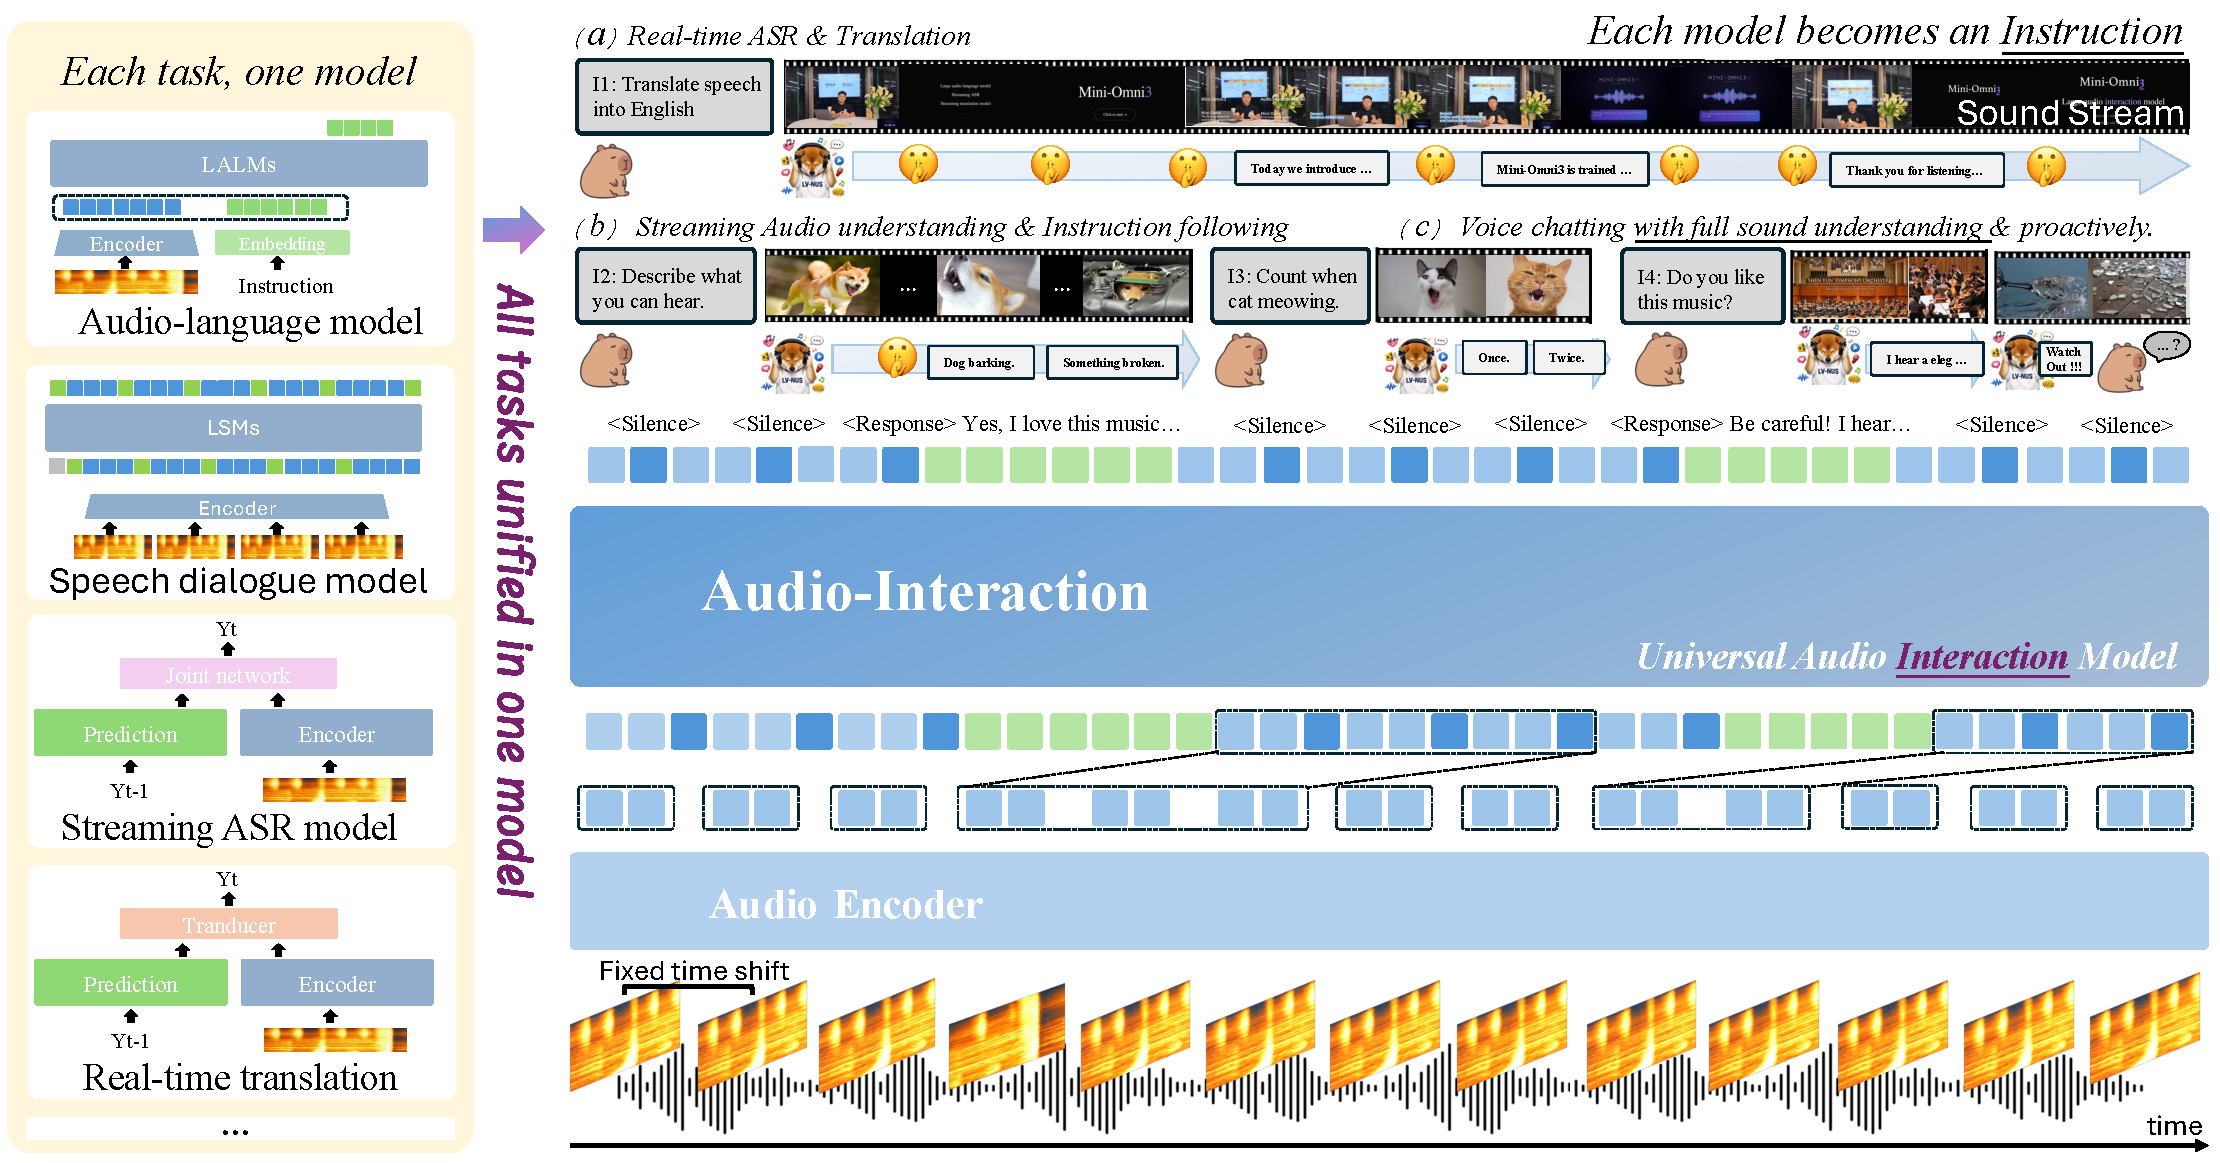
\includegraphics[width=0.95\linewidth]{fig/new_main_newnane.pdf}
    \caption{Human listening is a continuous activity. We take in sound moment by moment and judge for ourselves when a reaction is called for. Current audio models work the opposite way: they wait for a finished recording, answer once, and handle only one kind of task per system. \textsc{Audio-Interaction} closes this gap by processing sound as it arrives and judging, step by step, when to speak and when to hold back—letting one model cover what previously took many specialized ones.}
    \label{fig:main}
\end{figure}


\section{Audio-Interaction}
\vspace{-2mm}
\subsection{Overview}
\vspace{-2mm}
% \textsc{Audio-Interaction} extends large audio language models from offline clip-based processing to a general streaming audio-language setting. In contrast to existing systems that rely on carefully segmented audio clips, \textsc{Audio-Interaction} operates directly on continuous audio streams: it incrementally consumes incoming audio chunks, updates its understanding of the evolving acoustic context, and autonomously decides whether to remain silent or respond. This streaming formulation unifies a wide range of capabilities within a single framework, covering not only standard tasks such as audio understanding, spoken dialogue, and automatic speech recognition, but also streaming-native behaviors including online audio instruction following, real-time translation, and proactive full-audio interaction. To realize this paradigm, we further develop an efficient asynchronous inference framework, construct a large-scale training corpus of 260{,}000 hours, and introduce \textsc{ProactiveSound-Bench} for evaluating proactive intervention triggered by auditory signals.

 \textsc{Audio-Interaction}  bridges the gap between conventional offline, clip-based audio language models and a general streaming audio-language setting. As shown in figure~\ref{fig:main}, conventional LALMs operate on fixed inputs, $y = f(x, \mathcal{A})$, where $\mathcal{A}$ is the complete utterance and $x$ the text instruction; only after the full signal is observed is a response produced. In contrast,  \textsc{Audio-Interaction}  operates directly on continuous audio streams, incrementally consuming audio chunks and autonomously deciding whether to remain silent or respond:
\begin{equation}
    (d_t,\, r_t) = f\!\left(a_{\leq t},\; d_{<t},\; r_{<t}\right),
\end{equation}
where $a_t$ is the current audio chunk, $d_t$ is the \emph{streaming intervention decision}, and $r_t$ is the generated response. This \emph{perceive--decide--respond} loop unlocks a broad spectrum of capabilities: from speech translation to \underline{\emph{simultaneous interpretation}}, from speech dialogue to \underline{\emph{open-domain audio discussion}}, from audio understanding to \underline{\emph{audio instruction following}}, and even \underline{\emph{proactive assistance}} triggered solely by audio content without any explicit instruction.
\vspace{-1mm}
%  \textsc{Audio-Interaction}  aims to bridge the gap between conventional offline, clip-based audio language models and a general streaming audio--language setting, motivated by the fact that \emph{interactivity} and \emph{real-time responsiveness} are intrinsic to the nature of audio. Conventional audio language models are designed for offline, fixed-input inference: they take a complete audio utterance and a text instruction as input, and produce a response only after the full signal has been observed, i.e., $y = f(x, \mathcal{A})$, where $\mathcal{A}$ denotes the full audio utterance and $x$ the text instruction. In contrast,  \textsc{Audio-Interaction}  operates directly on continuous audio streams, incrementally consuming audio chunks and autonomously deciding whether to remain silent or respond:

% \vspace{-5mm}
% \begin{equation}
%     (d_t,\, r_t) = f\!\left(a_t,\; a_{t-1}, d_{t-1}, r_{t-1},\; a_{t-2}, d_{t-2}, r_{t-2},\; \cdots,\; a_0, d_0, r_0\right),
% \end{equation}
% \vspace{-6mm}

% where $a_t$ is the current audio chunk, $d_t$ is the \emph{streaming intervention decision}, and $r_t$ is the generated response. This \emph{perceive--decide--respond} loop enables real-time audio understanding and semantically grounded decision-making, unlocking a broad spectrum of capabilities: from speech translation to \underline{\emph{simultaneous interpretation}}, from speech dialogue to \underline{\emph{open-domain audio discussion}}, from audio understanding to \underline{\emph{audio instruction following}}, and even \underline{\emph{proactive assistance}} triggered solely by audio content without any explicit instruction.\vspace{-1mm}

% We then present the complete training pipeline and practical challenges of  \textsc{Audio-Interaction} , including realistic streaming data simulation, streaming training and inference, as well as the construction of \textsc{StreamAudio-2M}, a \textbf{260{,}000}-hour training corpus, and \textsc{ProactiveSound-Bench}, a benchmark for evaluating proactive audio understanding and assistive response without explicit user instruction.

\subsection{Streaming Data Construction}
\label{sec3.2: Streaming Data Construction} 
\vspace{-1.5mm}

\noindent
\begin{minipage}[t]{0.5\textwidth}
\textbf{Time-frequency joint preprocessing module.} We apply a lightweight time-frequency preprocessing module to make each audio segment smoother, more natural, and better aligned for downstream stitching. The module jointly regularizes temporal gaps and spectral continuity by iteratively clipping excessive internal silence (\texttt{silence\_cut}), estimating background noise from low-energy regions (\texttt{noise\_profile}) and removing it in the frequency domain (\texttt{denoise}), then locating the densest informative span (\texttt{core\_locate}) and refining both boundaries with half-chunk alignment $\delta=\frac{1}{2}$ of \textsc{Audio-Interaction} and short-window spectral smoothing $\omega$ (\texttt{boundary\_norm} $\rightarrow$ \texttt{spec\_smooth}). An early loop stabilizes silence/noise statistics, and if the final silence clipping still changes the segment, the process returns to Stage~1 for another pass. The overall procedure is summarized in Algorithm~\textcolor{red}{1}.

\end{minipage}
\hfill
\begin{minipage}[t]{0.48\textwidth}
\vspace{-12pt}
\footnotesize

\begin{algorithm}[H]
\caption{TFJP Module Pipeline}
\begin{algorithmic}[1]
\State \textbf{Input:} audio $x$, silence limit $\tau$, max iters $K$, smooth window $\omega$, align step $\delta$
\For{$k=1$ to $K$}
    \hfill {\color{blue}// S1--2: cut and norm.}
    \State $x \gets \texttt{silence\_cut}(x,\tau)$; $n \gets \texttt{noise\_profile}(x)$; $x \gets \texttt{denoise}(x,n)$
    \If{\texttt{stable}$(x,n)$} \textbf{break} \EndIf
\EndFor
\State $r \gets \texttt{core\_locate}(x)$ \hfill {\color{blue}// S3: localization}
\State $\tilde{x} \gets \texttt{boundary\_norm}(x,r,\tau,\delta)$ \hfill {\color{blue}// S4: trim.}
\State $\tilde{x} \gets \texttt{spec\_smooth}(\tilde{x},\omega)$
\State $x' \gets \texttt{silence\_cut}(\tilde{x},\tau)$ \hfill {\color{blue}// final check}
\If{\texttt{changed}$(x',\tilde{x})$} $x \gets x'$; \textbf{goto S1} \Else \Return $x'$ \EndIf
\end{algorithmic}
\end{algorithm}

\end{minipage}


\begin{figure}[t]
\centering
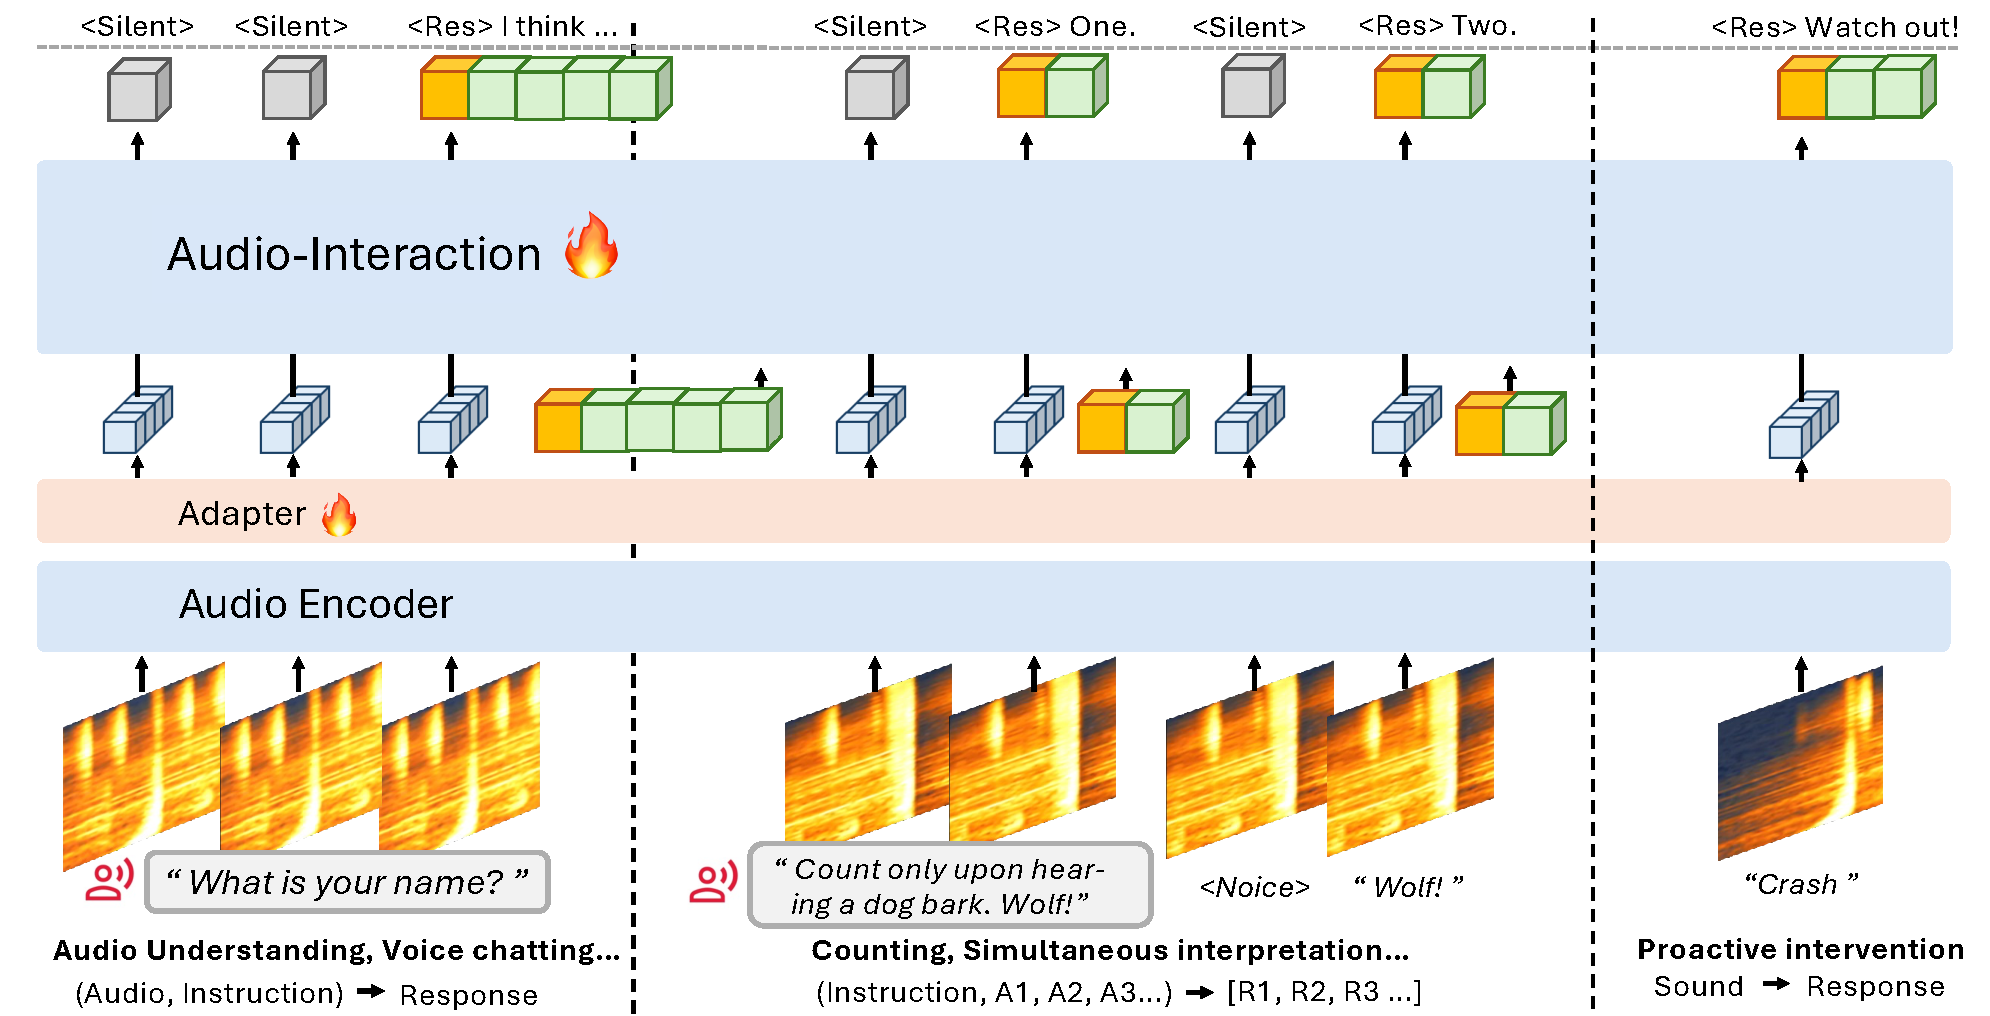
\includegraphics[width=0.95 \linewidth]{fig/soundfkow.pdf}
\caption{The training framework of \textsc{SoundFlow}. Audio signals, intermediate representations, and supervision signals are organized into a unified temporal sequence, and a streaming training strategy jointly optimizes language modeling and response triggering, enabling \textsc{Audio-Interaction} to decide when to respond or remain silent across diverse real-time tasks.
}
\vspace{-2mm}
\label{figure2-overview}
\end{figure}
% \textbf{TFLP module.} We apply a lightweight time-frequency preprocessing module to make each audio segment smoother, more natural, and better aligned for downstream stitching. The core idea is to jointly 
% \noindent
% \begin{minipage}[t]{0.5\textwidth}
% regulate temporal gaps and spectral continuity: overlong internal silence is first compressed, background noise is estimated from low-energy regions and removed in the frequency domain, the most informative core span is then localized, and the retained segment is finally refined at both boundaries. Concretely, the pipeline consists of silence normalization (\texttt{silence\_norm}), noise estimation and spectral denoising (\texttt{noise\_profile} $\rightarrow$ \texttt{denoise}), density-based core localization (\texttt{core\_locate}), and boundary normalization with local spectral smoothing (\texttt{boundary\_norm} $\rightarrow$ \texttt{spec\_smooth}). To match the downstream generation grid, boundary adjustment is constrained by a half-chunk alignment of Audio-Interaction, denoted by $\delta=\frac{1}{2}$ chunk, while smoothing is controlled by a short window $\omega$. A lightweight early loop stabil-
% \end{minipage}
% \hfill
% \begin{minipage}[t]{0.48\textwidth}
% \vspace{-12pt}
% \footnotesize

% \begin{algorithm}[H]
% \caption{TFLP module}
% \begin{algorithmic}[1]
% \State \textbf{Input:} audio $x$, silence limit $\tau$, max iters $K$, smooth window $\omega$, align step $\delta$
% \For{$k=1$ to $K$} 
%     \hfill {\color{blue}// S1--2: Normalization}
%     \State $x \gets \texttt{silence\_norm}(x,\tau)$; $n \gets \texttt{noise\_profile}(x)$; $x \gets \texttt{denoise}(x,n)$ 
%     \If{\texttt{stable}$(x,n)$} \textbf{break} \EndIf
% \EndFor
% \State $r \gets \texttt{core\_locate}(x)$ \hfill {\color{blue}// S3: localization}
% \State $\tilde{x} \gets \texttt{boundary\_norm}(x,r,\tau,\delta)$ \hfill {\color{blue}// Stage 4: boundary normalization}
% \State $\tilde{x} \gets \texttt{spec\_smooth}(\tilde{x},\omega)$ 
% \State $\tilde{x} \gets \texttt{silence\_norm}(\tilde{x},\tau)$ \hfill {\color{blue}// final check}
% \State \Return $\tilde{x}$
% \end{algorithmic}
% \end{algorithm}

% \end{minipage}
% izes silence and noise statistics, and a final consistency check ensures that no excessive internal gap remains after boundary refinement.

\textbf{Hierarchical Audio Event Selection.} Another key challenge in constructing streaming audio data is how to organize discrete (\texttt{audio}, \texttt{instruction}, \texttt{response}) segments into \underline{\textit{long, multi-turn audio}} \underline{\textit{streams that remain coherent and consistent with real-world commonsense}}. A straightforward solution is \textit{random concatenation}, i.e., sampling audio clips independently and stitching them into a long sequence. However, this strategy is suboptimal, as event conflicts across clips (e.g., a car horn occurring while a speaker is talking) can easily break contextual consistency and impair the model's understanding of the evolving scene. To address this issue, we adopt a \textbf{hierarchical event curation pipeline} when composing mixed streaming data, which contains: 

\vspace{-1mm}
\underline{\textit{(i) scenario planning:}} We first use an LLM to plan a complete high-level scenario from randomly matched audio annotations, where each scenario contains multiple topics or sub-events. 

\vspace{-1mm}
\underline{\textit{(ii) event refinement:}} We then refine each topic into a sequence of concrete audio events and assign a corresponding audio clip to each event. 

\vspace{-1mm}
\underline{\textit{(iii) clip grounding:}} The final audio clips are obtained through two mechanisms, \textit{retrieval} or \textit{generation}. For retrieval, the model searches an audio clip database, selects the \textbf{top-3} most relevant candidates, and verifies their suitability. When no retrieved clip is sufficiently appropriate, we instead invoke an audio generation model to synthesize the required event. This hierarchical design yields long-form streaming audio with substantially better semantic coherence and environmental plausibility.


% \textbf{audio事件层次化选择} 另一个构造流式音频数据的难点是如何组织离散的音频-指令-回答片段到一个长，多轮，符合现实常识的音频流数据。一种简单的做法是random拼接，随机从数据中取出音频片段拼接成长音频。但是这样的拼接是sub optimal的，for由于冲突（eg 说话时有汽车鸣笛）引起的模型对上下文的失败理解。因此，我们在拼接混合数据时，使用了层次化事件的策划机制。我们会首先用LLM基于随机匹配的音频标注策划一个完整事件，包含多个主题。 然后每个主题会重新确认音频事件，每个事件最终获取音频。音频共有两种机制，搜索或获取。模型会在音频clip数据库中搜索，选择top-3相关的音频，确认是否可用。 or 会调用音频生成模型生成。



%  转换离线模型到流式模型，重要的决定性因素是能否构建出和现实中发生的极相似的长音频数据。由于很难获取大量的自然生活中的长音频 with caption，拼接是更scalable的方式。核心挑战包括：（1）上下文事件合理性：模型很可能会学坏基于上下文的理解和进一步的决策， 如果训练于不合理拼接的音频和标注。 （2）严格的时间对齐和自然流畅度保证模型学会介入时机。 在本节中，我们介绍两个流式数据构造时的核心方法。

% 时间-频谱联合前处理模块： 

% Model architecture

% streaming spe_token prediction
% Audio-Interaction的推理和训练机制如图2所示。音频不是以整个clip的形式输入，而是被切分成chunk，which时间是我们精心设计的400ms， 流式输入模型。接着，模型自行决定通过special_token此时是否需要继续聆听，例如句子还没说完或者音频中还没听到答案，或者在准确的时机介入。总的来说，模型的反应可以为：

% 类似下面这个
% \[
% d_t = f_{\mathrm{det}}(x_t, H_t), \qquad
% y_t =
% \begin{cases}
% \varnothing, & d_t=\texttt{<silent>},\\
% f_{\mathrm{fast}}(x_t, H_t), & d_t=\texttt{<fast\_intervention>},\\
% f_{\mathrm{final}}(x_t, H_t, \tilde{I}_t), & d_t=\texttt{<full\_assistance>},
% \end{cases}
% \]

\vspace{-2mm}
\subsection{Streaming Training}
\vspace{-1mm}
\textbf{Streaming modeling.}  As illustrated in Figure~2, both training and inference in our framework follow a fully streaming paradigm. Instead of processing a complete audio clip at once, the model incrementally consumes fixed-length audio chunks. In our implementation, each chunk spans 400\,ms, balancing responsiveness and acoustic completeness. At each step, the model predicts a \emph{single special token} $d_t \in \{\texttt{<silent>}, \texttt{<response>}\}$ to determine whether it should continue listening or start responding. Intuitively, the model should remain silent when the current utterance is still incomplete or when the observed evidence is insufficient, and respond once enough information has been accumulated or timely intervention is required. Formally,
\[
d_t, r_t = f_{\mathrm{det}}(a_t, C_t), \qquad
r_t =
\begin{cases}
\varnothing, & d_t=\texttt{<silent>},\\[4pt]
f_{\mathrm{resp}}(a_t, C_t), & d_t=\texttt{<response>},
\end{cases}
\]
where $a_t$ is the current audio chunk and $C_t$ denotes the streaming context up to step $t$. If $d_t=\texttt{<silent>}$, the model emits no textual content and continues consuming subsequent audio chunks. Otherwise, it switches from streaming listening to autoregressive response generation. This formulation casts streaming interaction as a unified sequential process, allowing the model to jointly learn \emph{when} to respond and \emph{what} to generate in real-time spoken interaction.
% \textbf{Streaming modeling.}  As illustrated in Figure~2, both training and inference in our framework follow a fully streaming paradigm. Rather than processing the entire audio clip at once, the model consumes audio incrementally in fixed-length chunks. In our implementation, the chunk length is set to 400\,ms to balance responsiveness and acoustic completeness. At each streaming step, the model predicts a control token that determines whether it should continue listening or start responding. Intuitively, the model should remain silent when the current utterance is still incomplete or when the answer cannot yet be reliably inferred from the observed audio, and it should respond once sufficient evidence has been accumulated or when timely intervention is required. Formally, given the interleaved history of audio chunks and previous decisions, the next streaming decision is modeled as
% \[
% d_t, y_t= f_{\mathrm{det}}(x_t, H_t), \qquad
% y_t =
% \begin{cases}
% \varnothing, & d_t=\texttt{<silent>},\\[4pt]
% f_{\mathrm{resp}}(x_t, H_t), & d_t=\texttt{<response>},
% \end{cases}
% \]
% where the history state is defined as
% \[
% H_t = (x_0, d_0, y_0, x_1, d_1, y_1, \ldots, x_{t-1}, d_{t-1}, y_{t-1}).
% \]
% where $d_{t+1} \in \{\texttt{<silent>}, \texttt{<response>}\}$. If the model predicts \texttt{<silent>}, it emits no textual content and continues consuming subsequent audio chunks. If it predicts \texttt{<response>}, it transitions from streaming listening to autoregressive response generation. This formulation unifies turn-taking and content generation into a single sequential decision process, enabling the model to jointly learn both \emph{when} to respond and \emph{what} to generate in real-time spoken interaction.

\textbf{Context Memory and Comprehension-Aware Silence Training.}  During training, we observe two critical failure modes: \underline{\textit{(1) insufficient context retention}}, where the model tends to overlook earlier context due to the prevalence of noisy or semantically empty segments in long training sequences; to address this issue, we introduce \emph{history review} training by inserting questions about preceding content into later positions of the sequence, explicitly encouraging long-range contextual retrieval. \underline{\textit{(2) false triggering}}, where the model tends to respond to interaction-irrelevant acoustic events; to mitigate this issue, we incorporate a large amount of silent audio verified by the agents in \textsc{ProactiveSound-Bench} to require no response, thereby strengthening the model's ability to remain silent unless intervention is truly warranted.
% Streaming Model Training

% - streaming eos prediction
% - 长序列建模 and negative samples.
% - training loss
\textbf{Dual-loss Multi-step Streaming Conversion.}  \textsc{Audio-Interaction} is initialized from Qwen2.5-Omni-3B, which offers a strong performance--efficiency trade-off at a compact scale and is well suited for low-latency streaming inference. Since the special streaming control token $\texttt{<Spe\_token>}$ constitutes a new prediction target and is central to streaming interaction, we optimize it with a dedicated streaming objective in addition to the standard language modeling objective. Specifically, the overall training loss is defined as
\[
\mathcal{L}
=
\frac{1}{N}\sum_{j=1}^{N}
\left(
\underbrace{-\log P_\theta\!\left(t_j \mid \mathcal{H}_j\right)}_{\mathcal{L}_{\mathrm{LM}}}
+
\lambda\underbrace{-\log P_\theta\!\left(s_j \mid \mathcal{H}_j\right)}_{\mathcal{L}_{\mathrm{stream}}}
\right),
\]
where $t_j$ denotes the target text token, $s_j$ denotes the target streaming control token, $\mathcal{H}_j$ denotes the corresponding decoding context, and $\lambda$ controls the relative weight of the streaming objective.

Let $\mathcal{A}^{\mathrm{ins}}$ denote the audio instruction, $\mathcal{A}^{\mathrm{in}}$ the input audio stream, and $\mathcal{T}$ the target response. The training pipeline consists of four stages. \underline{\textit{(1) Format training}}: we use offline data to teach the model the target sequence format and the usage of $\texttt{<Spe\_token>}$, using samples of the form $(\mathcal{A}^{\mathrm{ins}}, \mathcal{A}^{\mathrm{in}} \rightarrow \mathcal{T})$. \underline{\textit{(2) Adapter training}}: we train the adapter to map chunk-wise acoustic representations into the language model space while keeping the training format unchanged. \underline{\textit{(3) Large-scale streaming supervised training}}: we jointly optimize the adapter and language model on core capabilities, including audio understanding, automatic speech recognition, and spoken dialogue, using $(\mathcal{A}^{\mathrm{ins}} \rightarrow \mathcal{T})$ and $(\mathcal{A}^{\mathrm{ins}}, \mathcal{A}^{\mathrm{in}} \rightarrow \mathcal{T})$. \underline{\textit{(4) Instruction-following fine-tuning}}: we further train the model on complex streaming behaviors, including continuous assistance, comprehension-aware intervention, and proactive response, using interleaved sequences such as $(\mathcal{A}^{\mathrm{ins}}, \mathcal{A}^{\mathrm{in}}_1, \mathcal{T}_1, \mathcal{A}^{\mathrm{in}}_2, \mathcal{T}_2, \ldots)$, $(\mathcal{A}^{\mathrm{ins}}, \mathcal{A}^{\mathrm{in}}_1, \mathcal{A}^{\mathrm{in}}_2, \mathcal{T}, \mathcal{A}^{\mathrm{in}}_3, \mathcal{T}, \ldots)$, and $(\mathcal{A}^{\mathrm{in}} \rightarrow \mathcal{T})$.


\subsection{Stabilizing Asynchronous Inference via FIFO Scheduling.}
\vspace{-2mm}

Real-time audio encoding and the model's special-token-based silence--response mechanism can introduce waiting conflicts and scheduling inconsistencies under complex interaction patterns. To

\begin{minipage}[t]{0.52\linewidth}
\vspace{-4.3mm}
 mitigate this issue, we adopt an \textbf{asynchronous} inference scheme with \textbf{FIFO} scheduling. As illustrated in Fig.~\ref{fig:fifo_inference}, the encoder continuously processes streaming audio chunks and appends their acoustic representations to a temporally ordered queue. At each event step $t$, the incoming chunk $x_t$ is encoded into $\mathbf{a}_t$ and appended to the queue $\mathcal{Q}_t$. The decoding process is conditionally triggered based on the last generated token $r_{t-1}$. Specifically, if $r_{t-1} \in \{\texttt{<eos>}, \texttt{<silent>}\}$, the model consumes the queued features $\mathcal{Q}_t$ and produces the next output $r_t$. Otherwise, the system remains waiting until subsequent audio chunks arrive. This deployment 
\end{minipage}
\hfill
\begin{minipage}[t]{0.45\linewidth}
\vspace{-2mm}
\centering
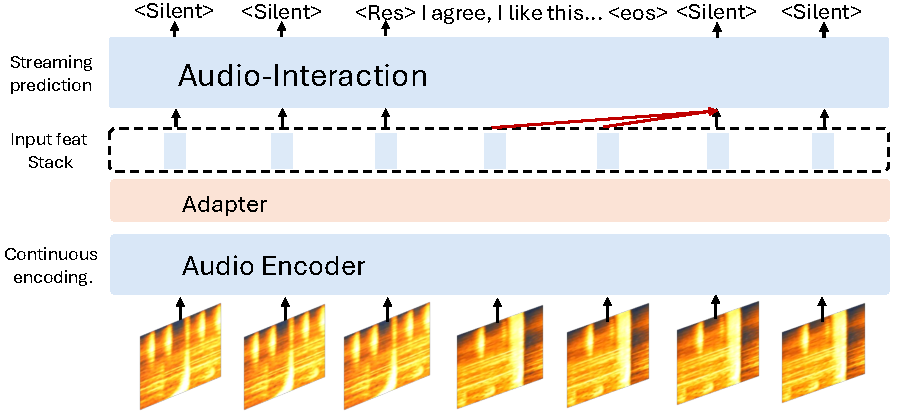
\includegraphics[width=\linewidth]{fig/figure4-inference-newname.pdf}
\vspace{-4mm}
\captionof{figure}{SoundFlow's FIFO-scheduled asyn chronous streaming inference. Audio chunks are appended to temporal queue; decoding is triggered when decoder is not speaking.}
\label{fig:fifo_inference}
\end{minipage}

\vspace{-1.7mm}
scheme fully eliminates inference stalling, while reducing the first-frame latency for resuming listening after response completion by $4.5\times$. Together, these improvements enable both stable and low-latency streaming inference.




%\subsection{FIFO Deployment for Stable Inference.}Because real-time audio encoding and the model's special-token-based silence--response mechanism can introduce waiting conflicts and scheduling inconsistencies under complex interaction patterns, we design the inference framework following a FIFO principle. Specifically, the encoder continuously processes newly arrived audio chunks in a streaming loop, and the resulting acoustic representations are appended to a queue in temporal order. The decoder consumes encoded chunks from this queue whenever the model remains silent or finishes a response. This FIFO design preserves temporal consistency between streaming input and generation, and thereby stabilizes inference under asynchronous encoding--decoding dynamics.

\begin{figure}[!t]
    \centering
    \includegraphics[width=0.95\linewidth]{fig/dataset.png}
    \vspace{-1mm}
    \caption{\textsc{StreamAudio-2M} is a dataset built for streaming audio interaction, pairing long-form, real-world-simulated audio with token-level annotations. It jointly trains the model to interact in real time grounded in context while covering 7 foundational capabilities across 28 sub-tasks.}
    \vspace{-4mm}
    \label{fig:streamaudio_main}
\end{figure}

% 现有的音频数据集都是Audio_clip with. Ins，Res。 不能用来训练流式audio模型。另一种可能是获取视频背景音等长音频，however无法保证有效的训练模型该有的能力。 所以我们创建了StreamAudio-2M,一个使用拼接，with 方法of sec 3.2，创建的专为流式音频大模型训练的数据集。 数据in streamaudio-2M features: 1. 格式上长达5-15min的音频，with 各种音频事件，模拟流式音频大模型会听到的音频。 2. 不是所有的声音都需要回复，模型被训练于基于上下位理解再需要回复的位置和内容。 3. 内部拥有大量语音指令，训练模型保持基础任务能力（ASR,S2TT,Audio-QA），与音频指令遵循，基于音频的主动介入等新任务能力。
\vspace{-2mm}
\section{StreamAudio-2M Dataset}
\label{sec:data_section}
\vspace{-2mm}
\subsection{Overview}
\label{sec:data_overview}
\vspace{-2mm}


Existing audio datasets are dominated by short \textit{(clip, instruction, response)} triplets~\citep{kong2024audioflamingo,chu2024qwen2}, which are fundamentally misaligned with streaming audio LLMs that operate over continuous streams and must jointly decide \emph{when} to respond and \emph{what} to produce. To bridge this gap, we introduce \textit{StreamAudio-2M}, as shown in Figure~\ref{fig:streamaudio_main} a large-scale streaming-native corpus that covers the full spectrum of streaming audio interaction through \textbf{7 major categories}: \textit{\underline{Audio Agent,}} \textit{\underline{Proactive Respond, Voice Chatting, Streaming Audio Understanding, Following Music, Real-time}} \textit{\underline{ASR and Streaming Translation }}, further partitioned into \textbf{28 streaming sub-tasks}. In total, the corpus comprises \textbf{2.6M} items totaling \textbf{302k hours}, where each sample is a \textbf{3--15 turn} heterogeneous interaction with interleaved events and sparse, context-dependent response cues. The detailed task composition and proportions are illustrated in Figure~\ref{fig:overview}.

% \vspace{-2mm}
% \subsection{Overview}
% \label{sec:data_overview}
% \vspace{-2mm}

% Existing audio datasets consist of short \textit{(clip, instruction, response)} triplets~\citep{kong2024audioflamingo,chu2024qwen2audio} that are fundamentally misaligned with streaming audio LLMs operating over continuous streams. We therefore introduce \textit{StreamAudio-2M}, where each sample forms a \textbf{5--15 min} heterogeneous audio stream with interleaved events and sparse, context-dependent response cues, forcing the model to jointly learn \emph{when} to respond and \emph{what} to produce. The corpus comprises \textbf{2.6M} items spanning \textbf{11 conventional and 7 streaming-native tasks}, totaling \textbf{302k hours}, and is organized into four components: \textit{\underline{single-task samples}} (\textbf{40\%}) covering dialogue, Audio-QA, and other foundational tasks; \textit{\underline{scenario-level composite data}} (\textbf{30\%}) with co-occurring heterogeneous events; \textit{\underline{advanced complex-task data}} (\textbf{20\%}) for instruction following; and \textit{\underline{proactive intervention}} (\textbf{10\%}), a novel signal critical for streaming interaction. See Figure.~\ref{app:bench:categories} for the full domain and task taxonomy.

% Existing audio datasets predominantly consist of short \textit{(clip, instruction, response)} triplets~\cite{af2,qwen2audio}, which are fundamentally misaligned with streaming audio LLMs that must operate over continuous, unbounded acoustic streams. A seemingly plausible alternative—mining long-form video audio (e.g., background tracks)—fails to guarantee coverage of the capability spectrum required for robust training. To bridge this gap, we introduce \textit{StreamAudio-2M}, a corpus purpose-built for streaming audio LLMs via the concatenation-based construction in Sec.~3.2. Each sample forms a \textbf{5--15 min} heterogeneous audio stream with interleaved events, within which response-worthy cues are \emph{sparse} and context-dependent, requiring the model to jointly learn \emph{if/when} to respond (\(\textit{when}\)) and \emph{what} to produce (\(\textit{what}\)); meanwhile, densely embedded speech instructions both preserve core capabilities (ASR, S2TT, Audio-QA) and enable higher-level behaviors such as audio-grounded instruction following and proactive intervention.

% \textbf{Data Statistic}   \textit{StreamAudio-2M} comprises \textbf{2.6M} items spanning \textbf{11 conventional tasks} and \textbf{7 newly introduced streaming tasks}, totaling \textbf{302k hours} of audio. The corpus consists of four complementary components: \textit{\underline{single-task samples}} (\textbf{40\%}), covering dialogue, Audio-QA, and other foundational tasks; \textit{\underline{scenario-level composite data}} (\textbf{30\%}), with co-occurring heterogeneous events; \textit{\underline{advanced complex-task data}} (\textbf{20\%}), targeting instruction following; and \textit{\underline{proactive intervention}} (\textbf{10\%}), a novel signal \textbf{indispensable} for interactive streaming agents yet largely unexplored~\cite{af2,qwen2audio}. See Fig.~\ref{fig:taxonomy} for detailed \textit{domain taxonomy} and \textit{task taxonomy}.

\vspace{-2.4mm}
\subsection{Curation Pipeline}
\label{sec:curation_pipeline}
\vspace{-2mm}

The pipeline proceeds as follows. \textbf{(i) Data Collection.} As shown in
Figure~\ref{fig:overview}, our sources are drawn from a wide range of well-established
real-world datasets to ensure proximity to real distributions and robustness, including
dialogue corpora (MOSS), ASR corpora (CommonVoice, GigaSpeech,
LibriSpeech~\citep{panayotov2015librispeech}, VoxPopuli), speech translation data
(CoVoST2~\citep{wang2021covost}, AISHELL), music and audio-QA prompts (FMA,
AudioSet~\citep{gemmeke2017audio}), yielding $\sim$1.64M foundational task items
($\sim$8{,}900 hours); on top of these we add $\sim$171k acoustic-event clips
(AudioSet events, AudioX~\citep{tian2025audiox}, ElevenLabs) and noise sources
(MUSAN~\citep{snyder2015musan}, WHAM!~\citep{wichern2019wham},
DNS-Challenge~\citep{timcheck2023intel}) used only as environmental conditioning.
\textbf{(ii) Preprocessing.} Textual sources are converted into speech with multi-voice
CosyVoice and verified by LLM rewriting and ASR checking. \textbf{(iii) Sequence
Concatenation.} Validated instances are composed into streaming sequences following
Section~\ref{sec3.2: Streaming Data Construction}, with dual-track environmental noise
superimposed. \textbf{(iv) Token-level Annotation.} The resulting sequences are converted
into $\langle\text{input ids}, \text{labels}\rangle$ pairs.

\begin{figure}[t]
\centering
% ===================== 左：原图 (a)(b) =====================
\begin{minipage}[t]{0.66\textwidth}
  \centering
  \vspace{0pt}
  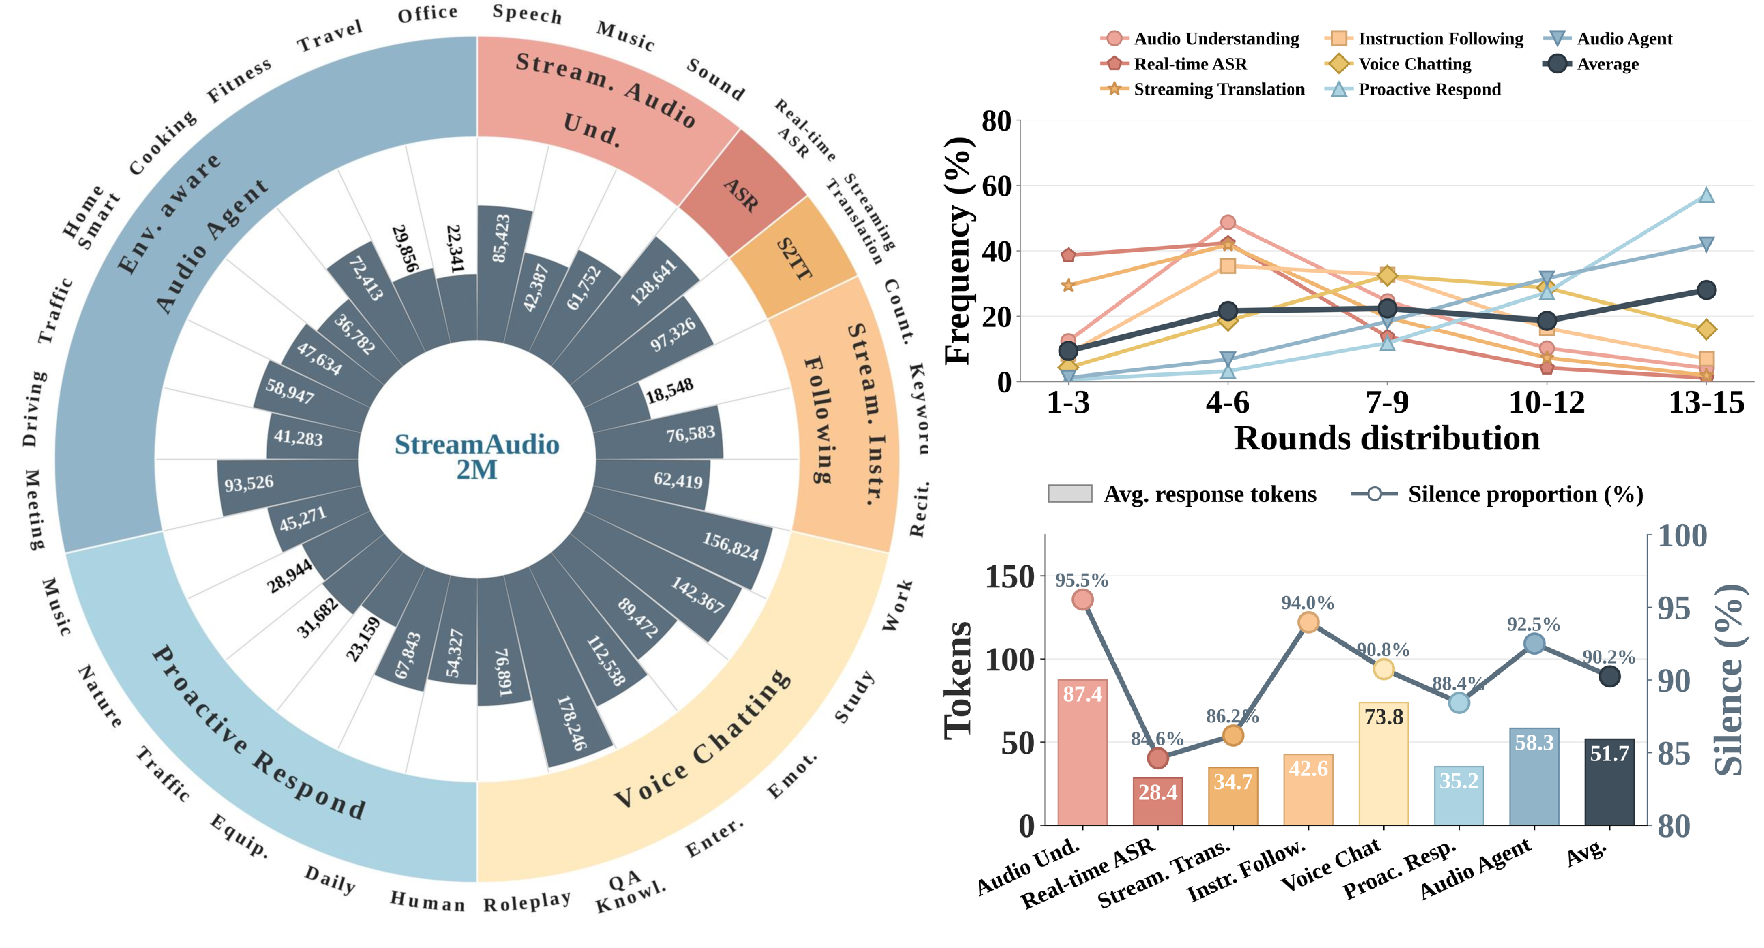
\includegraphics[width=\linewidth]{fig/final.pdf}
\end{minipage}%
\hfill
% ===================== 右：重构后的表格 (c) =====================
\begin{minipage}[t]{0.32\textwidth}
  \centering
  \vspace{0pt}

  % ---------- palette: 与 (a) 旭日图一致 ----------
  \definecolor{cVC}{HTML}{E7C95F}\definecolor{cIF}{HTML}{D9B441}
  \definecolor{cAA}{HTML}{6E9FC4}\definecolor{cPR}{HTML}{A6CFE0}
  \definecolor{cASR}{HTML}{D9544D}\definecolor{cAU}{HTML}{E59182}
  \definecolor{cS2T}{HTML}{E08A2E}
  \definecolor{hdrbg}{HTML}{2C3A57}\definecolor{rowbg}{HTML}{F4F6FA}
  \definecolor{srcgy}{HTML}{8A8F99}

  % ---------- helpers ----------
  \newcommand{\chip}[1]{\textcolor{#1}{\rule[0em]{.6em}{.6em}}}
  \newcommand{\pbar}[2]{\textcolor{#1}{\rule[-.08em]{#2}{.6em}}}
  \newcommand{\src}[1]{\textcolor{srcgy}{\fontsize{4.7}{5.4}\selectfont #1}}

  \scriptsize
  \setlength{\tabcolsep}{3pt}
  \renewcommand{\arraystretch}{1.0}

  \resizebox{0.95\linewidth}{!}{%   <<< 关键：整表缩放到列宽
  \begin{tabular}{@{}l r @{\hspace{5pt}} l@{}}
    \rowcolor{hdrbg}
    \textbf{\textcolor{white}{Task}} & \textbf{\textcolor{white}{\#Item}} & \textbf{\textcolor{white}{Share}} \\[2pt]

    \rowcolor{rowbg}\chip{cVC}~Voice Chatting & 539k & \pbar{cVC}{.90cm}\,23.1\% \\
    \rowcolor{rowbg}\multicolumn{3}{@{}l@{}}{\hspace{1.2em}\src{MOSS, GammaCorpus-Fact-QA}}\\[1.5pt]

    \chip{cIF}~Str. Instr. Follow. & 487k & \pbar{cIF}{.81cm}\,20.8\% \\
    \multicolumn{3}{@{}l@{}}{\hspace{1.2em}\src{UltraChat, Magpie-Pro, BellGroup, COIG-CQIA \textit{+2}}}\\[1.5pt]

    \rowcolor{rowbg}\chip{cAU}~Str. Audio Und. & 382k & \pbar{cAU}{.64cm}\,16.4\% \\
    \rowcolor{rowbg}\multicolumn{3}{@{}l@{}}{\hspace{1.2em}\src{AudioSet (Open/Choice), FMA (Open/Choice)}}\\[1.5pt]

    \chip{cS2T}~Str. Translation & 357k & \pbar{cS2T}{.60cm}\,15.3\% \\
    \multicolumn{3}{@{}l@{}}{\hspace{1.2em}\src{CoVoST 2 (En$\leftrightarrow$CN), AISHELL}}\\[1.5pt]

    \rowcolor{rowbg}\chip{cASR}~Real-time ASR & 270k & \pbar{cASR}{.45cm}\,11.6\% \\
    \rowcolor{rowbg}\multicolumn{3}{@{}l@{}}{\hspace{1.2em}\src{CommonVoice, GigaSpeech, LibriSpeech, VoxPopuli}}\\[1.5pt]

    \chip{cPR}~Proactive Res. & 171k & \pbar{cPR}{.28cm}\,7.3\% \\
    \multicolumn{3}{@{}l@{}}{\hspace{1.2em}\src{AudioSet (events), AudioX, ElevenLabs}}\\[1.5pt]

    \rowcolor{rowbg}\chip{cAA}~Env. Audio Agent & 130k & \pbar{cAA}{.21cm}\,5.5\% \\
    \rowcolor{rowbg}\multicolumn{3}{@{}l@{}}{\hspace{1.2em}\src{MOSS, AudioSet (Desc./Open), WHAM!, DNS, MUSAN}}\\[3pt]

    \rowcolor{hdrbg}
    \multicolumn{3}{@{}c@{}}{\textcolor{white}{%
      \textbf{2.34M}\,items \;\textbullet\; \textbf{7.49M}\,rounds \;\textbullet\; \textbf{66.7K}\,hrs}}\\
  \end{tabular}}
  
\end{minipage}

\caption{Statistics of StreamAudio-2M. \textbf{(a)} The capability taxonomy spans seven core capabilities of a streaming audio model. \textbf{(b)} Round distribution, average response tokens, and silence proportion across tasks. \textbf{(c)} Statistics of source data.}
\vspace{-2mm}
\label{fig:overview}
\end{figure}


% \begin{figure}[!t]
% \centering
% \includegraphics[width=1.0 \linewidth]{fig/figure3-data.png}
% \caption{Overview of our data resources. (a--b)~Modality distribution and hierarchical task taxonomy across both \textsc{StreamAudio-2M} and \textsc{ProactiveSound-Bench}. (c)~\textsc{ProactiveSound-Bench} statistics. The bottom panel illustrates the four-stage data curation pipeline: collection, preprocessing, concatenation, and annotation.}
% \label{figure3-data}
% \end{figure}

% \textbf{Stage 1: Data Collection.}
% As shown in Table~\ref{tab:streamaudio_data}, we curate $\sim$1.64M foundational task items ($\sim$7,830 hours) from well-established corpora, including MOSS~\cite{moss} for dialogue, AudioX~\cite{audiox}, ElevenLabs~\cite{elevenlabs}, and AudioSet~\cite{audioset} for acoustic events, LibriSpeech~\cite{librispeech} for ASR, CoVoST2~\cite{covost2} for S2TT, AudioSet and AF-3~\cite{af3} together with Gemini-generated pairs for Audio-QA, and MUSAN~\cite{musan}, WHAM!~\cite{wham}, and DNS-Challenge~\cite{dns} as noise sources. These corpora collectively span dialogue, acoustic events, speech recognition, translation, reasoning QA, and ambient noise, providing the raw material upon which the \textit{TFJP} module and \textit{hierarchical event concatenation} (Sec.~\ref{sec:3.2}) operate to synthesize the final streaming corpus.% \paragraph{Curation Pipeline.}
% The pipeline in Figure~\ref{figure1-overview} has four stages. \emph{Data collection} aggregates raw items via web search, data organization, and LLM generation. \emph{Preprocessing} synthesizes text sources into speech with multi-voice CosyVoice and verifies fidelity through LLM rewriting and ASR checking. \emph{Sequence concatenation} composes validated instances into streaming sequences following Section~\ref{sec:data}, superimposing dual-track environmental noise. \emph{Token-level annotation} extracts encoder features and emits the $\langle\text{input ids}, \text{labels}\rangle$ pairs used for training. Details are in Appendix~\ref{app:data}.



% \label{sec:streamaudio2m}
% % ---------- Sidebar Grouped Table (polished) ----------
% \begin{wraptable}{r}{0.5\textwidth}
% \vspace{-20pt}
% \centering
% \small
% \setlength{\tabcolsep}{3pt}
% \renewcommand{\arraystretch}{0.85}
% \caption{Resources composing StreamAudio-2M.}
% \label{tab:data_sources}
% \begin{tabular}{@{}llrr@{}}
% \toprule
% \textbf{Task} & \textbf{Resource} & \textbf{\#Inst.} & \textbf{Hours} \\
% \midrule
% Dialogue                   & MOSS                  & 450k & 5{,}600 \\
% \addlinespace[2pt]
% \arrayrulecolor{black!25}\cmidrule{1-4}\arrayrulecolor{black}
% \addlinespace[2pt]
% \multirow{3}{*}{Audio Events}
%                            & AudioX                &  60k &   50 \\
%                            & ElevenLabs            &  25k &   21 \\
%                            & AudioSet              &  15k &   21 \\
% \addlinespace[2pt]
% \arrayrulecolor{black!25}\cmidrule{1-4}\arrayrulecolor{black}
% \addlinespace[2pt]
% ASR                        & LibriSpeech           & 170k &  330 \\
% \addlinespace[2pt]
% \arrayrulecolor{black!25}\cmidrule{1-4}\arrayrulecolor{black}
% \addlinespace[2pt]
% S2TT                       & CoVoST2               &  70k &  140 \\
% \addlinespace[2pt]
% \arrayrulecolor{black!25}\cmidrule{1-4}\arrayrulecolor{black}
% \addlinespace[2pt]
% \multirow{3}{*}{Audio Und.}
%                            & AudioSet+Gemini       & 150k &  210 \\
%                            & AudioSet              & 100k &  140 \\
%                            & AF-3                  & 250k &  700 \\
% \addlinespace[2pt]
% \arrayrulecolor{black!25}\cmidrule{1-4}\arrayrulecolor{black}
% \addlinespace[2pt]
% Text SFT                   & Public corpora        & 350k &  --  \\
% \midrule
% \multirow{4}{*}{Noise}
%                            & MUSAN                 & 929  &   60 \\
%                            & WHAM!                 & --   &   80 \\
%                            & DNS-Challenge         & --   &  300 \\
%                            & AudioSet              & --   &  180 \\
% \bottomrule
% \end{tabular}
% \vspace{-20pt}
% \end{wraptable}

% Mini-Omni~3 must understand audio, react to environmental events, and sustain multi-turn exchanges. We accordingly collect six complementary task families: multi-turn dialogue (450k), proactive audio events (100k), ASR (170k), S2TT (70k), audio understanding (500k), and text-only instruction tuning (350k), plus $620$ hours of environmental noise across $12$ acoustic scenes, as listed in Table~\ref{tab:data_sources}.
% \paragraph{Curation Pipeline.}
% The pipeline in Figure~\ref{figure1-overview} has four stages. \emph{Data collection} aggregates raw items via web search, data organization, and LLM generation. \emph{Preprocessing} synthesizes text sources into speech with multi-voice CosyVoice and verifies fidelity through LLM rewriting and ASR checking. \emph{Sequence concatenation} composes validated instances into streaming sequences following Section~\ref{sec:data}, superimposing dual-track environmental noise. \emph{Token-level annotation} extracts encoder features and emits the $\langle\text{input ids}, \text{labels}\rangle$ pairs used for training. Details are in Appendix~\ref{app:data}.

\vspace{-1.5mm}
\subsection{Proactive-Sound-Bench}
\label{sec:proactive_bench}
 \vspace{-1.5mm}
\textbf{ProactiveSound-Bench} evaluates proactive streaming response through \textbf{644} \textit{human-designed} acoustic events, each requiring the model to correctly trigger or abstain within a continuous stream. Events span 6 top-level categories with $17$ sub-categories, and are organized into two tiers, \emph{Single} and \emph{Multiple}, where the \emph{Single} tier tests single-event decisions and the \emph{Multiple} tier concatenates same-category events to probe sustained intervention against distractors, with average accuracy as the final metric. Per-category statistics are provided in Table~\ref{tab_meso_definitions}.

% \section{Experiments}
% \label{sec:experiments}
 
% \subsection{Settings}
% \label{sec:settings}

% \paragraph{Benchmarks.}
% We evaluate Mini-Omni~3 on five benchmarks covering the full capability spectrum of a streaming audio language model: \textbf{(1) ASR}: LibriSpeech (clean/other); \textbf{(2) S2TT}: CoVoST2 (En$\leftrightarrow$Zh); \textbf{(3) Spoken Dialogue}: Llama Questions and Web Questions (single-/multi-turn), together with the AlpacaEval and SD-QA subsets of VoiceBench; \textbf{(4) Audio Understanding}: MMAU (Sound/Music/Speech); \textbf{(5) Proactive Streaming Response}: our proposed Proactive-Sound-Bench.
 
% \paragraph{Baselines.}
% We compare Mini-Omni~3 against a broad range of audio language models falling into four categories: \textbf{(a) specialized task models}: Whisper-large-v3, Canary, among others; \textbf{(b)audio LLMs}: Qwen2-Audio, Kimi-Audio, SALMONN, Audio-Reasoner,among others; \textbf{(c) omni LLMs}: Qwen2.5-Omni 3B/7B, miniCPM-o-4.5, among others; and \textbf{(d) streaming speech LLMS}: Moshi, Freeze-Omni, LLama-Omni2, among others. Details are in Appendix ~\ref{Apendix}.
 
% \paragraph{Implementation Details.}
% Mini-Omni~3 is built on Qwen2.5-Omni-3B and trained on StreamAudio-2M for $4$ epochs based on $8$ NVIDIA L40s GPUs. The optimizer is AdamW with a learning rate of $2\!\times\!10^{-4}$, cosine schedule. The encoder frame rate is set to $0.04$~s per audio token, and a streaming decision is made every $0.4$~s ($10$ tokens). More implementation details are listed in Appendix~\ref{app:impl}.

% \subsection{Main Results}
% \label{sec:main_results}

% \begin{table}[t]
% \centering
% \caption{\textbf{Audio understanding results on MMAU.} Accuracy(\%) is reported across three audio domains under text and audio instructions. \{so, mu, sp\} indicates whether a model supports sound, music, and speech understanding, respectively.}
% \label{tab:mmau}
% \vspace{0pt}
% \scriptsize
% \setlength{\tabcolsep}{3pt}
% \renewcommand{\arraystretch}{0.8}
% \resizebox{\textwidth}{!}{%
% \begin{tabular}{@{}l c c cccc cccc@{}}
% \toprule
% \multirow{2.5}{*}{\textbf{Model}}
%   & \multirow{2.5}{*}{\textbf{Size}}
%   & \multirow{2.5}{*}{\textbf{\{so, mu, sp\}}}
%   & \multicolumn{4}{c}{\textbf{Text instruction}}
%   & \multicolumn{4}{c}{\textbf{Audio instruction}} \\
% \cmidrule(lr){4-7} \cmidrule(lr){8-11}
%   &  &  & Sound & Music & Speech & Avg.
%        & Sound & Music & Speech & Avg. \\
% \midrule
% \multicolumn{11}{@{}l}{\cellcolor{headerblue}\textit{\textbf{Large Audio Language Models}}} \\
% Audio Flamingo 2          & 3B   & Y Y Y & 71.47 & 70.96 & 44.74 & 62.40 & 1.50 & 1.49 & 0.35 & 1.16 \\
% Qwen2-Audio-Instruct      & 8.4B & Y Y Y & 54.95 & 50.98 & 42.04 & 49.20 & 22.32 & 19.16 & 16.31 & 19.41 \\
% Voxtral-Mini              & 3B   & Y Y Y & 58.56 & 49.70 & 43.53 & 50.60 & 46.08 & 34.13 & 30.50 & 37.24 \\
% Audio-Reasoner            & 8.4B & Y Y Y & 60.06 & 64.30 & 60.70 & 61.71 & 0.0 & 0.0 & 0.0 & 0.0 \\
% \multicolumn{11}{@{}l}{\cellcolor{headerblue}\textit{\textbf{Omni Language Models}}} \\
% Qwen2.5-Omni              & 3B   & Y Y Y & 65.36 & 48.94 & 57.78 & 57.81 & 51.81 & 44.01 & 29.79 & 42.51 \\
% Qwen2.5-Omni              & 7B   & Y Y Y & 67.87 & 69.16 & 59.76 & 65.60 & 60.54 & 50.90 & 35.11 & 49.58 \\
% Phi-4-multimodal-instruct & 7B   & Y Y Y & 60.97 & 52.87 & 52.83 & 55.56 & 44.65 & 27.84 & 21.99 & 31.75 \\
% Baichuan-Omni-1.5         & 11B  & Y Y Y & 65.47 & 58.98 & 55.26 & 59.90 & 57.53 & 36.53 & 24.82 & 40.40 \\
% \multicolumn{11}{@{}l}{\cellcolor{headerblue}\textit{\textbf{Streaming Audio Language Models}}} \\
% \textcolor{gray}{[Base model (w/o SFT)]} & \textbf{3B} & Y Y Y & - & - & - & - & - & - & - & - \\
% \textbf{Ours (w/ SFT)} & \textbf{3B} & Y Y Y & - & - & - & - &  \best{65.63} & \best{57.93} & \best{39.68} & \beat{58.15}\\
% \bottomrule
% \end{tabular}%
% }
% \vspace{-6pt}
% \end{table}

% \begin{table}[t]
% \centering
% \caption{\textbf{Dialogue instruction-following and ASR \& S2TT results.}
% (a) Accuracy(\%) on LLama Questions and Web Questions for single- and multi-turn dialogue.
% (b) WER(\%,$\downarrow$) for ASR on LibriSpeech; BLEU($\uparrow$) for S2TT.}
% \label{tab:dialogue_asr}
% \vspace{0pt}

% \noindent
% \begin{subtable}[t]{0.58\textwidth}
% \centering
% \scriptsize
% \setlength{\tabcolsep}{3pt}
% \renewcommand{\arraystretch}{0.8}
% \begin{tabular}{@{}l c c c c c@{}}
% \toprule
% \multirow{2.5}{*}{\textbf{Model}}
%   & \multirow{2.5}{*}{\textbf{Type}}
%   & \multicolumn{2}{c}{\textbf{SpokenQA}}
%   & \multicolumn{2}{c}{\textbf{Voicebench}} \\
% \cmidrule(lr){3-4} \cmidrule(lr){5-6}
%   &  & LLama Q. & Web Q. & AlpacaEval & SD-QA \\
% \midrule
% \multicolumn{6}{@{}l}{\cellcolor{headerblue}\textit{\textbf{Full-duplex LALMs}}} \\
% Moshi                   & 7B & 62.20 & 26.30 & 2.01 & 15.01  \\
% Freeze-Omni             & 7B & 72.00 & 44.73 & 4.14  & -     \\
% \multicolumn{6}{@{}l}{\cellcolor{headerblue}\textit{\textbf{Dialogue LMs}}} \\
% Kimi-Audio-Instruct     & 7B & 79.33 & 70.20 & 4.46 & 63.12  \\
% \multicolumn{6}{@{}l}{\cellcolor{headerblue}\textit{\textbf{Omni LMs}}} \\
% LLama-Omni2             & 7B & 68.33 & 34.89 & 4.43  & -  \\
% Qwen2.5-Omni            & 3B & 66.00 & 27.95 & 4.32  &49.37  \\
% Qwen2.5-Omni            & 7B & 75.33 & 62.80 & 4.49 & 55.71 \\
% Baichuan-Omni-1.5       & 7B & 78.50 & 59.10 & 4.50 & 43.40 \\
% \multicolumn{6}{@{}l}{\cellcolor{headerblue}\textit{\textbf{Streaming LMs}}} \\
% \textcolor{gray}{[Base model (w/o SFT)]} & \textbf{3B} & - & - & - & - \\
% \textbf{Ours (w/ SFT)}  & \textbf{3B} & \best{0.0} & \best{0.0} & \best{0.0} & \best{0.0} \\
% \bottomrule
% \end{tabular}
% \subcaption{Dialogue instruction-following.}
% \label{tab:dialogue}
% \end{subtable}
% \hfill
% \begin{subtable}[t]{0.41\textwidth}
% \centering
% \scriptsize
% \setlength{\tabcolsep}{3pt}
% \renewcommand{\arraystretch}{0.8}
% \begin{tabular}{@{}l c c c c c@{}}
% \toprule
% \multirow{2.5}{*}{\textbf{Model}}
%   & \multirow{2.5}{*}{\textbf{Type}}
%   & \multicolumn{2}{c}{\textbf{ASR}}
%   & \multicolumn{2}{c}{\textbf{S2TT}} \\
% \cmidrule(lr){3-4} \cmidrule(lr){5-6}
%   &  & clean & other & en-zh & zh-en \\
% \midrule
% \multicolumn{6}{@{}l}{\cellcolor{headerblue}\textit{\textbf{Specialized}}} \\
% Whisper-v3        & 1.5B & 2.01 & 3.91 & -     & 14.36 \\
% Canary            & 1B   & 1.48 & 2.93 & -     & -     \\
% \multicolumn{6}{@{}l}{\cellcolor{headerblue}\textit{\textbf{General Audio LMs}}} \\
% Qwen2-Audio       & 7B   & 1.60 & 3.60 & 45.20 & 24.40 \\
% MinMo             & 7B   & 1.84 & 3.89 & 46.70 & 26.00 \\
% \multicolumn{6}{@{}l}{\cellcolor{headerblue}\textit{\textbf{Omni LMs}}} \\
% Qwen2.5-Omni      & 3B   & 2.87 & 5.90  & 39.50 & 18.17 \\
% Qwen2.5-Omni      & 7B   & 1.80 & 3.40  & 41.40 & 29.40 \\
% Phi-4-MM          & 5.6B & 1.69 & 3.82  & 46.30 & 22.39 \\
% \multicolumn{6}{@{}l}{\cellcolor{headerblue}\textit{\textbf{Streaming LMs}}} \\
% \textcolor{gray}{[Base model (w/o SFT)]} & \textbf{3B} & - & - & - & - \\
% \textbf{Ours (w/ SFT)} & \textbf{3B} & \best{0.0} & \best{0.0} & \best{55.22} & \best{35.21} \\
% \bottomrule
% \end{tabular}
% \subcaption{ASR \& S2TT.}
% \label{tab:asr}
% \end{subtable}

% \vspace{-6pt}
% \end{table}


% The question for \textsc{Audio-Interaction} is not whether a streaming model can match an offline one on familiar benchmarks, but whether moving to an always-on regime reveals capabilities offline models cannot express. Our results point to both, yielding three enhancements: \textit{\textbf{[Enh.1]}} streaming training preserves and in most cases improves offline capability; \textit{\textbf{[Enh.2]}} \textsc{Audio-Interaction} holds its ground when instructions themselves become audio, where competitors degrade; \textit{\textbf{[Enh.3]}} on knowing \textit{when to speak} rather than merely \textit{what to say}, \textsc{Audio-Interaction} is the only model that avoids the two failure modes that plague every existing baseline.

% \noindent\textit{\textbf{[Enh.1]} \textbf{Audio-Interaction pays no tax for streaming.}} Tab.~\ref{tab:mmau} and Tab.~\ref{tab:dialogue_asr} show that chunked listening and the extra streaming objective do not erode general skills. On MMAU, \textsc{Audio-Interaction} gains around 5 points of average accuracy over its Qwen2.5-Omni-3B initialization (+4.8\%); on CoVoST2 it adds 5 to 10 BLEU on both English and Chinese directions, closing most of the gap to 7B-scale systems; on SpokenQA it matches the base model. The only concession is a 3-point WER regression on LibriSpeech, an honest cost of replacing an utterance-level ASR head with a chunk-wise streaming decoder.

% \noindent\textit{\textbf{[Enh.2]} \textbf{Audio-Interaction is the only model that holds up when instructions become audio.}} In an always-on setting, instructions arrive as speech rather than text, and this is where existing models quietly break. Tab.~\ref{tab:mmau} shows Qwen2.5-Omni, Audio-Reasoner, and Voxtral-Mini all shedding 5 to 10 points of MMAU accuracy once instructions are spoken rather than typed, exposing a training-deployment mismatch that clean benchmarks have been masking. \textsc{Audio-Interaction} was trained exclusively on audio instructions, with every signal in StreamAudio-2M delivered through the streaming audio channel; we therefore evaluate it only under audio instructions (the empty text-instruction column in Tab.~\ref{tab:mmau}), where it leads all baselines. The asymmetry is the point: a model that never relied on a text-instruction shortcut has none to lose at deployment.

% \noindent\textit{\textbf{[Enh.3]} \textbf{Audio-Interaction is the only model with genuinely selective proactive response.}} On Proactive-Sound-Bench (Tab.~\ref{tab:proactive}), the baselines expose two failure modes. MiniCPM-o-4.5 reaches an average of 58.8 but a Resp. score near 0.0 across every tier, firing on nearly every event, a failure we call \textit{over-triggering}. Qwen2.5-Omni-7B and Kimi-Audio-Instruct show the opposite, \textit{context collapse}: average accuracy falls sharply as streams lengthen (Qwen2.5-Omni-7B drops from 58.23 to 28.91 between Single and Multiple-5). \textsc{Audio-Interaction} avoids both, posting the highest average and Resp. across all tiers and surpassing Gemini-3-Flash by roughly 15 points. This is no accident: Comprehension-Aware Silence Training (Sec.~\ref{sec:streaming_training}) teaches the model not merely \textit{what to say}, but \textit{whether this is the moment to say anything at all}, which is what separates a streaming audio LM from an offline one pretending to stream.

% \begin{table*}[t]
% \centering
% \scriptsize
% \setlength{\tabcolsep}{5pt}
% \renewcommand{\arraystretch}{0.8}
% \caption{Main results on the Proactive-Sound-Bench with updated categorization. \textit{Equip.} stands for Equipment, \textit{Resp.} denotes Selectivity RESPOND.}
% \begin{tabular}{@{}l!{\vrule width 0.4pt}l!{\vrule width 0.4pt}cccccc!{\vrule width 0.4pt}c!{\vrule width 0.4pt}c@{}}
% \toprule
% \multirow{2.5}{*}{\textbf{Model}}
%   & \multirow{2.5}{*}{\textbf{Type}}
%   & \multicolumn{6}{c!{\vrule width 0.4pt}}{\textbf{Category}}
%   & \multirow{2.5}{*}{\textbf{Avg.}}
%   & \multirow{2.5}{*}{\textbf{Resp.}} \\
% \cmidrule(lr){3-8}
%   &  & \textbf{Human} & \textbf{Daily} & \textbf{Equip.} & \textbf{Traffic} & \textbf{Nature} & \textbf{Music} & & \\
% \midrule

% \textbf{Qwen2.5-Omni-3B} & Single & 37.18 & 48.07 & 30.00 & 44.90 & 45.63 & 53.33 & 40.99 & 8.99 \\
% \rowcolor{multi3color}
%  & Multiple-3 & 28.85 & 42.46 & 17.86 & 36.73 & 17.48 & 40.00 & 29.28 & 7.89 \\
% \rowcolor{multi5color}
%  & Multiple-5 & 23.72 & 30.73 & 14.49 & 16.33 & 22.33 & 26.67 & 22.97 & 6.79 \\
% \midrule

% \textbf{Qwen2.5-Omni-7B} & Single & 54.49 & 72.93 & 47.86 & 53.06 & 55.34 & 53.33 & 58.23 & 8.99 \\
% \rowcolor{multi3color}
%  & Multiple-3 & 34.62 & 40.22 & 19.29 & 24.49 & 31.07 & 60.00 & 32.09 & 4.51 \\
% \rowcolor{multi5color}
%  & Multiple-5 & 28.85 & 35.20 & 16.67 & 22.45 & 34.95 & 46.67 & 28.91 & 4.53 \\
% \midrule

% \textbf{Kimi-Audio-Instruct} & Single & 39.10 & 61.33 & 28.57 & 28.57 & 26.21 & 26.67 & 39.91 & 14.98 \\
% \rowcolor{multi3color}
%  & Multiple-3 & 26.28 & 38.55 & 22.14 & 16.33 & 28.16 & 26.67 & 28.35 & 15.41 \\
% \rowcolor{multi5color}
%  & Multiple-5 & 25.64 & 37.43 & 15.22 & 18.37 & 19.42 & 13.33 & 24.84 & 11.32 \\
% \midrule

% \textbf{MiniCPM-o-4.5} & Single & 53.84 & 75.14 & 52.86 & 55.10 & 48.54 & 53.33 & 58.85 & 0.75 \\
% \rowcolor{multi3color}
%  & Multiple-3 & 53.21 & 75.42 & 52.86 & 55.10 & 47.57 & 53.33 & 58.87 & 0.00 \\
% \rowcolor{multi5color}
%  & Multiple-5 & 53.21 & 75.42 & 52.90 & 55.10 & 47.57 & 53.33 & 58.59 & 0.00 \\
% \midrule

% \textbf{Step-Audio} & Single &  9.62 &  7.73 &  4.29 & 12.24 & 14.56 &  6.67 &  8.85 & 21.35 \\
% \rowcolor{multi3color}
%  & Multiple-3 &  5.77 &  3.35 &  0.00 &  6.12 &  0.97 &  0.00 &  2.95 &  7.14 \\
% \rowcolor{multi5color}
%  & Multiple-5 &  8.33 &  2.79 &  0.00 &  0.00 &  3.88 &  0.00 &  3.44 &  8.30 \\
% \midrule

% \textbf{Gemini-3-Flash} & Single & 48.08 & 32.04 & 25.71 & 28.57 & 48.54 & 33.33 & 36.96 & 40.82 \\
% \rowcolor{multi3color}
%  & Multiple-3 & 59.61 & 47.49 & 40.00 & 53.06 & 56.31 & 53.33 & 50.77 & 38.35 \\
% \rowcolor{multi5color}
%  & Multiple-5 & 54.49 & 55.87 & 40.58 & 57.14 & 62.14 & 53.33 & 53.28 & 38.11 \\
% \midrule

% \textbf{Audio-Interaction (Ours)} & \textbf{Single} & \best{36.42} & \best{48.07} & \best{37.14} & \best{44.90} & \best{41.75} & \best{46.67} & \best{41.15} & \best{16.10} \\
% \rowcolor{multi3color}
%  & \textbf{Multiple-3} & \best{44.87} & \best{45.81} & \best{35.71} & \best{48.98} & \best{41.75} & \best{40.00} & \best{42.83} & \best{12.41} \\
% \rowcolor{multi5color}
%  & \textbf{Multiple-5} & \best{0.00} & \best{0.00} & \best{0.00} & \best{0.00} & \best{0.00} & \best{0.00} & \best{0.00} & \best{0.00} \\
% \bottomrule
% \end{tabular}
% \label{tab:main_results_updated}
% \end{table*}

% \begin{figure}[h]
% \begin{minipage}[t]{0.48\textwidth}
%     \centering
%     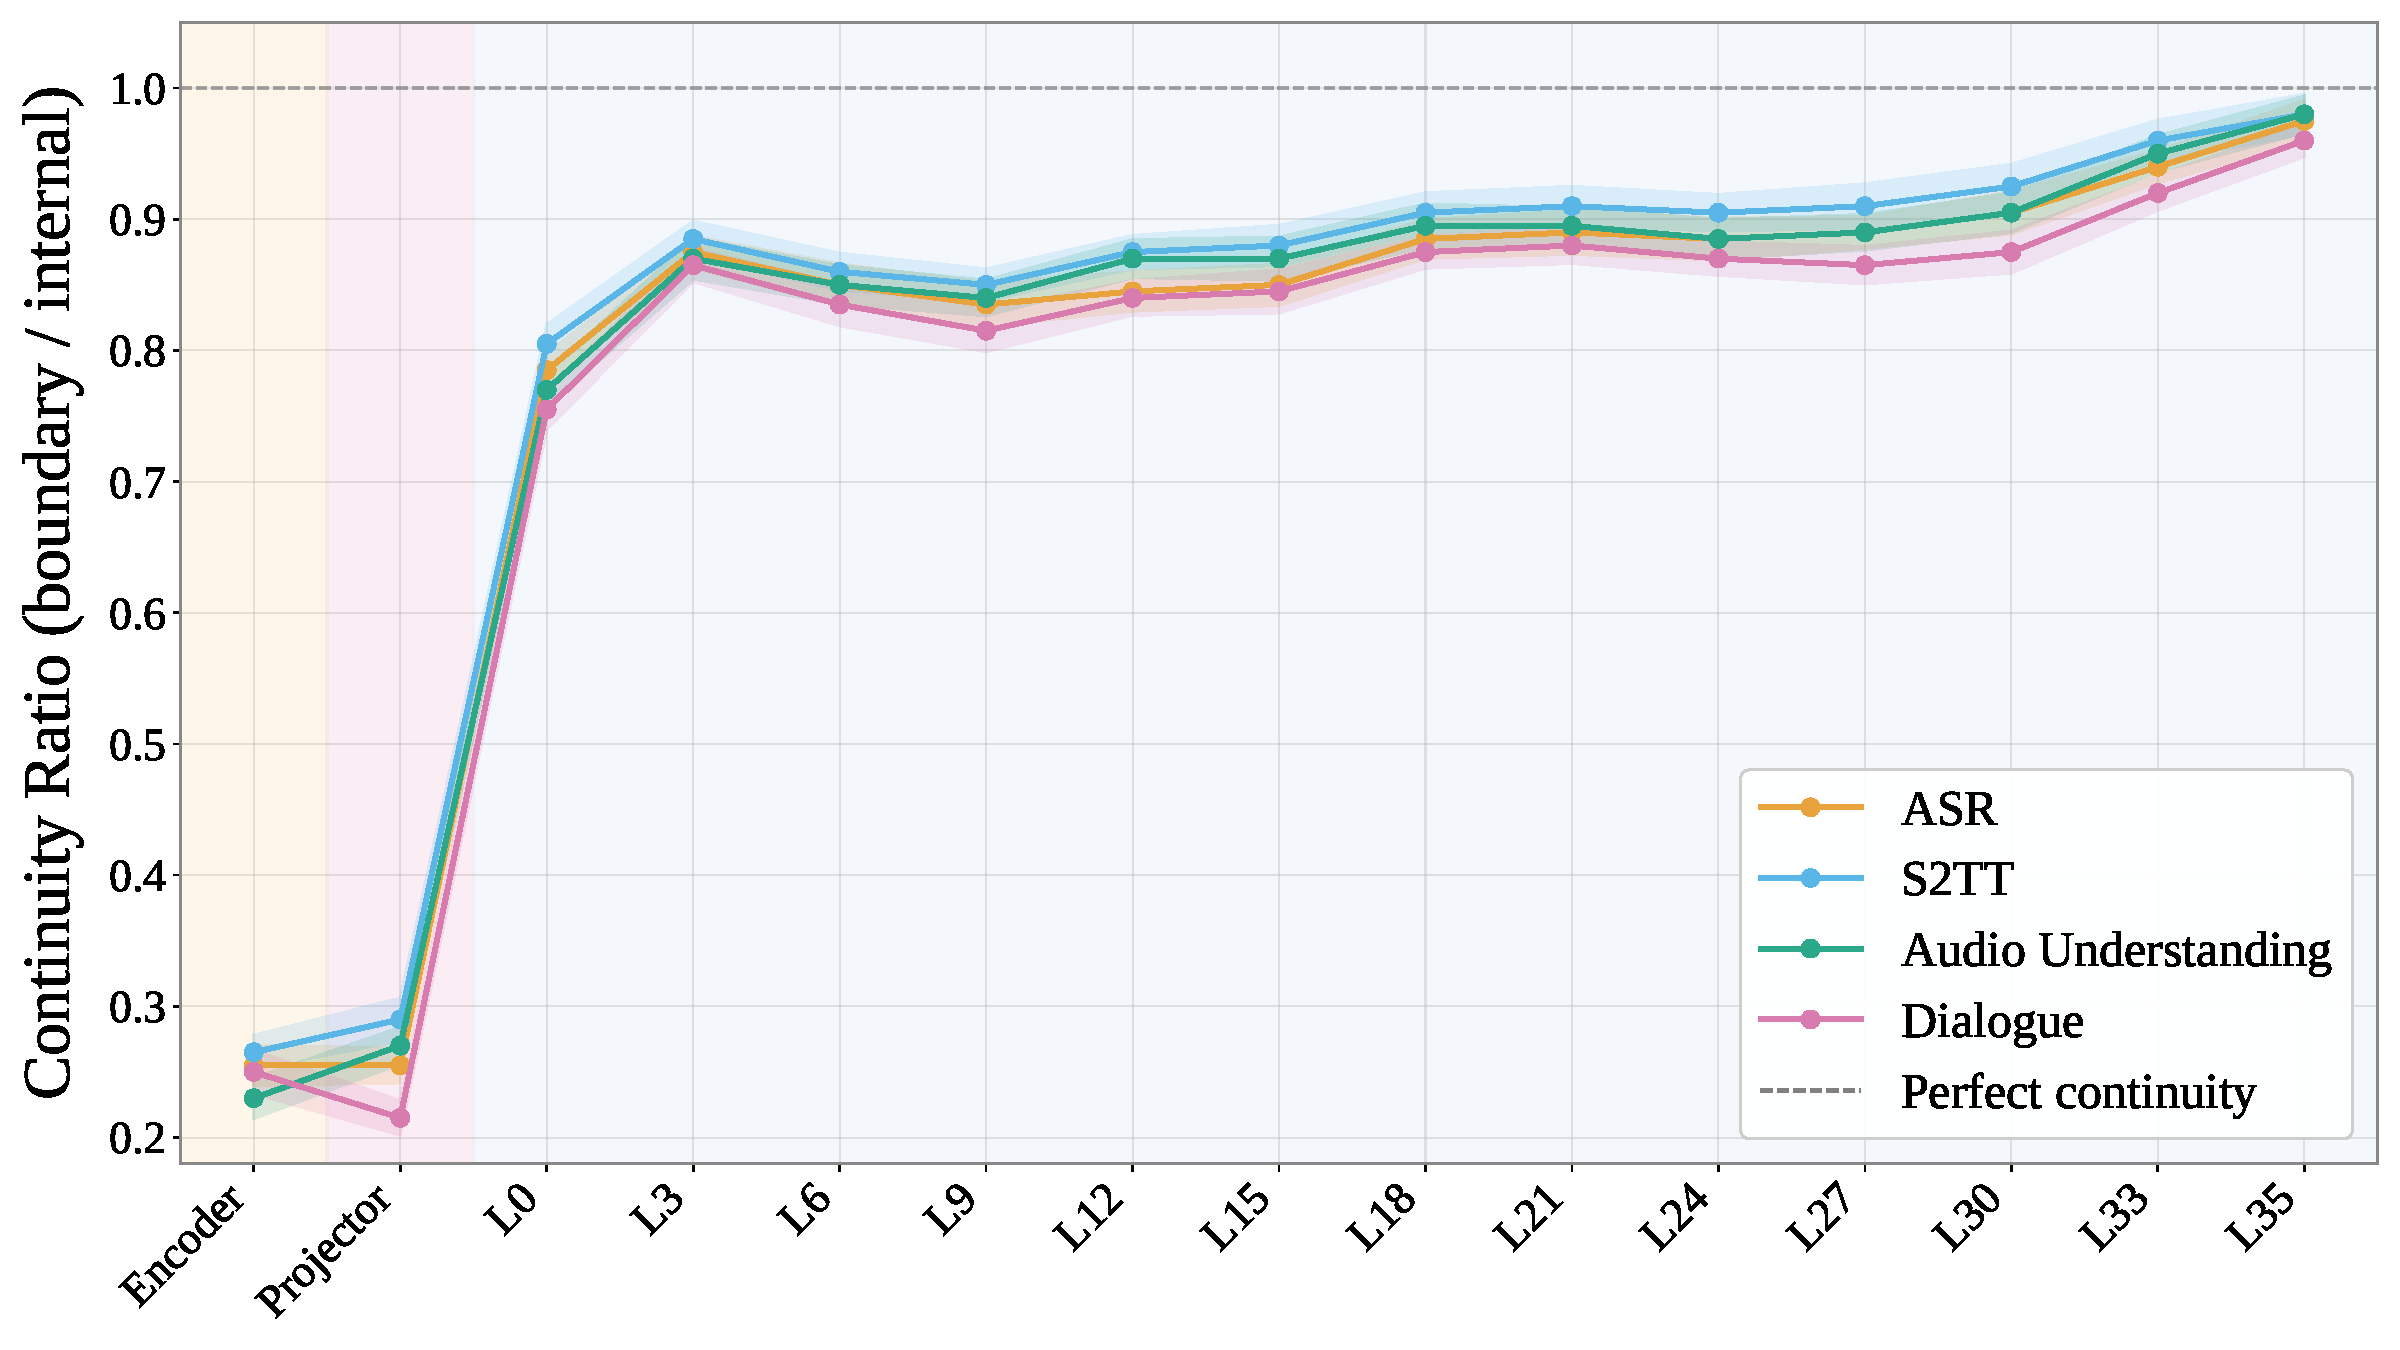
\includegraphics[width=\linewidth]{fig/cross_task_continuity.png}
%     \caption{Continuity ratio across processing stages. The projector barely moves the encoder's fragmented boundary; GPT Layer 0 alone recovers most of the continuity, and all four tasks follow the same curve.}
%     \label{fig:continuity}
% \end{minipage}%
% \hfill
% \begin{minipage}[t]{0.48\textwidth}
%     \centering
%     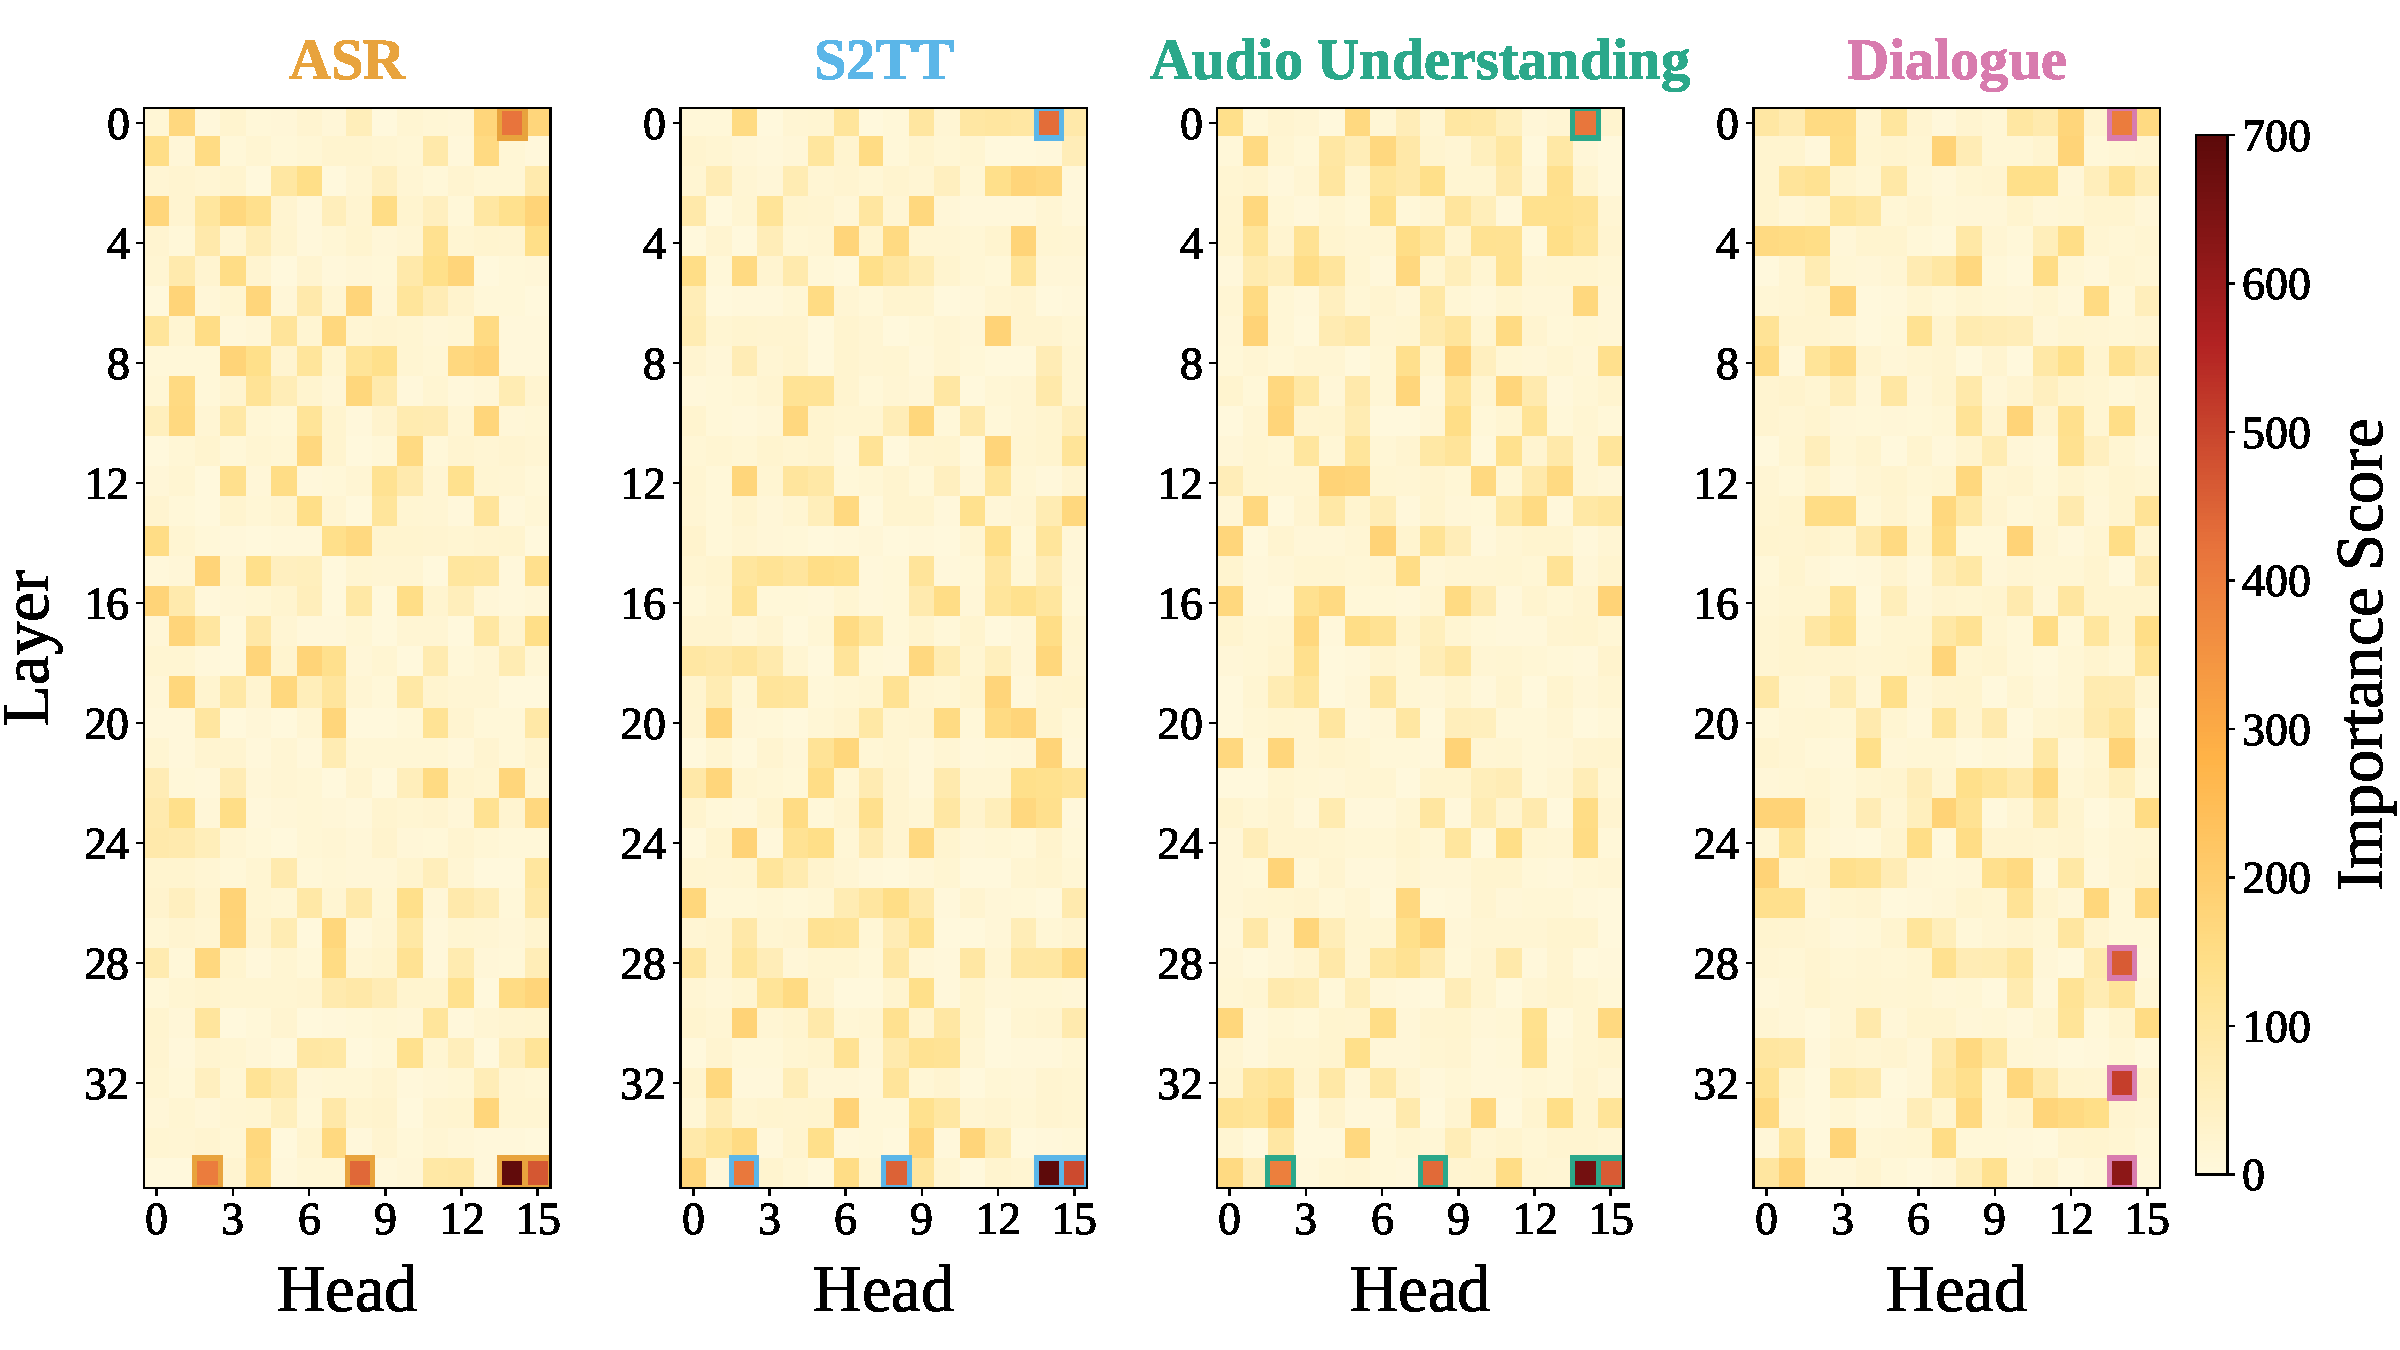
\includegraphics[width=\linewidth]{fig/fig3_cross_task_heatmaps.pdf}
%     \caption{Per-head importance across four tasks, measured via single-head ablation. A single head (L35H14) dominates every task; Spearman rank correlation across tasks exceeds 0.92.}
%     \label{fig:head_importance}
% \end{minipage}
% \end{figure}

% \subsection{Additional Analysis}

% To test whether \textsc{Audio-Interaction} embodies a streaming audio language model in its internal organization, not only in its benchmark scores, we probe the model along two axes, yielding two observations: \textit{\textbf{[Obs.1]}} cross-chunk continuity is reconstructed at GPT Layer 0, not by the projector; \textit{\textbf{[Obs.2]}} all four audio tasks share a single narrow backbone of attention heads.

% \noindent\textit{\textbf{[Obs.1]} \textbf{Cross-chunk continuity is reconstructed at GPT Layer 0.}} Since each 0.4\,s chunk is encoded with independent position embeddings and no cross-chunk encoder attention, the model has no architectural mechanism for representing time as continuous. We measure the resulting fragmentation with a continuity ratio, defined as boundary-pair cosine similarity divided by intra-chunk similarity (1.0 denotes seamless continuity). Fig.~\ref{fig:continuity} shows the encoder output sits at 0.25, four times lower than intra-chunk similarity; the projector, a trained linear map one might expect to handle alignment, moves this by less than 0.02. The entire recovery happens at GPT Layer 0, which lifts the ratio to 0.80 in a single step, with the first three layers reaching 0.87. Continuity is not encoded by the audio frontend; it is reconstructed at the earliest transformer layer with cross-chunk KV-cache access, because the streaming objective makes it the path of least resistance. All four tasks trace the same curve, identifying this as a property of the streaming regime rather than any task head.

% \noindent\textit{\textbf{[Obs.2]} \textbf{All four tasks share a single audio backbone.}} A model that passes four benchmarks can in principle have learned four independent circuits. We test this by zeroing each attention head in turn and measuring token-match degradation per task. Fig.~\ref{fig:head_importance} shows the result is stark: essentially all 576 heads have negligible effect, a single head (L35H14) dominates every task, removing it alone costs 0.88 token-match on S2TT, and Spearman rank correlation between any two task importance rankings exceeds 0.92. A cumulative ablation analysis (Appendix, Fig.~\ref{fig:cumulative_ablation}) further shows that removing just 10--20\% of heads collapses every task to near-zero token-match, with all four curves overlapping. The four tasks are not reading from four circuits; they share one narrow audio backbone, the parameter-level signature of a unified streaming objective that compresses capacity rather than allocating it per task. Streaming audio LMs thus appear substantially compressible along the head dimension, in a direction that is largely task-independent.

% \begin{figure}[t]
% \centering
% % ================= 上：折线图 =================
% \begin{subfigure}[b]{\textwidth}
%     \centering
%     \includegraphics[width=\linewidth]{fig/multi_audio_stability.pdf}
%     \subcaption{Capability stability across streams of 1--5 concatenated segments.}
%     \label{fig:ablation_stability}
% \end{subfigure}
% % ================= 下：两张表紧凑并排 ===============
% \begin{subfigure}[b]{0.48\textwidth}
%     \centering
%     \scriptsize
%     \setlength{\tabcolsep}{2pt}
%     \renewcommand{\arraystretch}{0.85}
%     \begin{tabular}{@{}llccc@{}}
%     \toprule
%     \textbf{Variant} & \textbf{Configuration} & \textbf{MMAU}$\uparrow$ & \textbf{Multi-5}$\uparrow$ & \textbf{Lat.}$\downarrow$ \\
%     \midrule
%     V1 & Qwen2.5-Omni base           & 57.8 & 23.0 & --  \\
%     V2 & V1 + our data (SFT)         & 60.5 & 25.7 & --  \\
%     V3 & V2 + streaming infer        & 54.1 & 20.3 & 268 \\
%     \midrule
%     V4 & Ours w/o preprocessing      & 56.8 & 34.5 & 210 \\
%     V5 & V4 + TFJP                   & 59.2 & 39.3 & 198 \\
%     \rowcolor{gray!15}
%     V6 & \textbf{Audio-Interaction (Full)}  & \textbf{62.3} & \textbf{45.5} & \textbf{192} \\
%     \bottomrule
%     \end{tabular}
%     \subcaption{Framework ablation.}
%     \label{fig:ablation_data}
% \end{subfigure}
% \hfill
% \begin{subfigure}[b]{0.50\textwidth}
%     \centering
%     \scriptsize
%     \setlength{\tabcolsep}{2pt}
%     \renewcommand{\arraystretch}{0.85}
%     \begin{tabular}{@{}lcccc@{}}
%     \toprule
%     \textbf{Variant} & \textbf{Chunk} & \textbf{Dialogue}$\uparrow$ & \textbf{MMAU}$\uparrow$ & \textbf{Lat.}$\downarrow$ \\
%     \midrule
%     w/o Inter. Tok.      & 0.4 & 61.2 & 58.4 & 310 \\
%     Chunk = 0.2\,s       & 0.2 & 63.8 & 59.1 & 185 \\
%     Chunk = 0.6\,s       & 0.6 & 65.7 & 62.5 & 295 \\
%     Chunk = 0.8\,s       & 0.8 & 65.9 & 62.8 & 378 \\
%     Non-streaming        & --  & 66.4 & 63.0 & --  \\
%     \midrule
%     \rowcolor{gray!15}
%     \textbf{Ours (Full)} & \textbf{0.4} & \textbf{66.0} & \textbf{62.3} & \textbf{192} \\
%     \bottomrule
%     \end{tabular}
%     \subcaption{Chunk size and design ablation.}
%     \label{fig:ablation_chunk}
% \end{subfigure}
% \caption{Ablation studies of Audio-Interaction. Accuracy / MMAU / Multi-5 / Dialogue are in \%; Latency in ms; Chunk in s. (a) Stream-length stability. (b) Framework and data recipe. (c) Chunk size and interaction token.}
% \label{fig:ablation_combined}
% \end{figure}

% \subsection{Ablation Study}
% We ablate \textsc{Audio-Interaction} along three axes in Fig.~\ref{fig:ablation_combined}.
% \textit{\underline{Framework and data are non-substitutable.}}
% V2 inherits our full data but trains offline, gaining 2.7 MMAU points yet leaving Multi-5 untouched; V4 uses the streaming objective on unprocessed data and recovers over 10 points on Multi-5 despite a slight MMAU drop, so learning \textit{when} to respond is not a data problem, and no data can substitute for it. V3, which streams at inference but not at training, collapses everywhere, confirming streaming is a training-time property. TFJP (V5) and Hierarchical Event Selection (V6) close the remaining gap and bring latency to 192\,ms.
% \textit{\underline{Proactivity is learned, not scheduled.}}
% Concatenating 1--5 independent segments into a single stream leaves all three metrics within 3\% of their single-segment values; only the $\pm 1\sigma$ band widens. A VAD- or interval-scheduled system would see its mean decay here, so a flat mean is direct evidence that the silent / response decision has been internalized.
% \textit{\underline{Chunk size depends on the interaction token, not the other way around.}}
% Shrinking chunks to 0.2\,s cuts latency but strips acoustic context and costs 3 MMAU points; enlarging to 0.6--0.8\,s doubles latency for under a point of gain. Removing the silent / response tokens, however, is worst on every axis and inflates latency to 310\,ms, meaning the token is the substrate that makes any chunk size meaningful. At 0.4\,s, \textsc{Audio-Interaction} reaches 62.3 MMAU and 66.0 dialogue accuracy against a non-streaming ceiling of 63.0 and 66.4, at roughly half the offline response delay.




%%%%%%%%%%%%%%%%%%%%%%%%%%%%%%%%%%%%%%%%%%%%%%%%%%%%%%%%%%%%



\vspace{-2mm}
\section{Experiments}
\label{sec:experiments}
 \vspace{-2mm}
 
\subsection{Settings}
\label{sec:settings}
\vspace{-2mm}

\paragraph{Benchmarks.}
We evaluate \textsc{Audio-Interaction} on \textbf{8} audio benchmarks spanning the full spectrum of LALM capabilities: \textbf{MMAU}~\citep{sakshi2024mmau} for general audio understanding across Sound, Music, and Speech; four spoken-dialogue benchmarks, including AlpacaEval~\citep{dubois2023alpacafarm}, SD-QA~\citep{faisal2021sd}, Llama Questions~\citep{nachmani2023spoken}, and Web Questions~\citep{berant2013semantic}, following the \textbf{VoiceBench}~\citep{chen2026voicebench} setting; \textbf{LibriSpeech}~\citep{panayotov2015librispeech} (clean/other) for speech recognition; \textbf{CoVoST2}~\citep{wang2021covost} (En$\leftrightarrow$Zh) for speech-to-text translation; and our newly proposed \textbf{Proactive-Sound-Bench} for evaluating proactive response capability.

\vspace{-2mm}
\paragraph{Baselines.}
We compare against three categories of models. \textbf{Audio LLMs}: Audio Flamingo 2~\citep{ghosh2025audio}, Qwen2-Audio~\citep{chu2024qwen2}, Voxtral-Mini~\citep{liu2025voxtral}, and Audio-Reasoner~\citep{audio-reasoner}. \textbf{Omni LLMs}: Qwen2.5-Omni~\citep{qwen25omni2025}, Baichuan-Omni-1.5~\citep{li2025baichuan}, and Phi-4-multimodal~\citep{abouelenin2025phi}. \textbf{Task-specialized models}: Whisper-large-v3~\citep{radford2023whisper} and Canary~\citep{sekoyan2025canary} for ASR; Moshi~\citep{defossez2024moshi}, Freeze-Omni~\citep{wang2024freeze}, and LLaMA-Omni2~\citep{fang2025llama} for streaming spoken dialogue. 

\vspace{-2mm}
\subsection{Main Results}
\label{sec:main_results}
\vspace{-2mm}

\begin{table}[t]
\centering
\caption{Results on the MMAU benchmark under text and audio instructions across three audio domains. \textbf{Stream.} and \textbf{Multi-turn} indicate streaming and multi-turn training support(\texttt{-} indicates not applicable).}
\label{tab:mmau}
\vspace{0pt}
\scriptsize
\setlength{\tabcolsep}{3pt}
\renewcommand{\arraystretch}{0.8}
\resizebox{\textwidth}{!}{%
\begin{tabular}{@{}l c c c cccc cccc@{}}
\toprule
\multirow{2.5}{*}{\textbf{Model}}
  & \multirow{2.5}{*}{\textbf{Size}}
  & \multirow{2.5}{*}{\textbf{Stream.}}
  & \multirow{2.5}{*}{\textbf{Multi-turn}}
  & \multicolumn{4}{c}{\textbf{Text instruction}}
  & \multicolumn{4}{c}{\textbf{Audio instruction}} \\
\cmidrule(lr){5-8} \cmidrule(lr){9-12}
  &  &  &  & Sound & Music & Speech & Avg.
       & Sound & Music & Speech & Avg. \\
\midrule
\multicolumn{12}{@{}l}{\cellcolor{headerblue}\textit{\textbf{Large Audio Language Models}}} \\
Audio Flamingo 2          & 3B   & \ding{55} & \ding{55} & \textbf{71.47} & \textbf{70.96} & 44.74 & \underline{62.40} & 1.50 & 1.49 & 0.35 & 1.16 \\
Qwen2-Audio      & 7B & \ding{55} & \ding{51} & 54.95 & 50.98 & 42.04 & 49.20 & 22.32 & 19.16 & 16.31 & 19.41 \\
Voxtral-Mini              & 3B   & \ding{55} & \ding{51} & 58.56 & 49.70 & 43.53 & 50.60 & 46.08 & 34.13 & 30.50 & 37.24 \\
Audio-Reasoner            & 8.4B & \ding{55} & \ding{55} & 60.06 & 64.30 & \textbf{60.70} & 61.71 & 20.48 & 26.65 & 13.48 & 20.57 \\
\multicolumn{12}{@{}l}{\cellcolor{headerblue}\textit{\textbf{Omni Language Models}}} \\
Qwen2.5-Omni              & 3B   & \ding{55} & \ding{51} & 65.36 & 48.94 & 57.78 & 57.81 & 51.81 & 44.01 & 29.79 & 42.51 \\
Qwen2.5-Omni              & 7B   & \ding{55} & \ding{51} & \underline{67.87} & \underline{69.16} & \underline{59.76} & \textbf{65.60} & \underline{60.54} & \underline{50.90} & \underline{35.11} & \underline{49.58} \\
Phi-4-multimodal & 5.6B   & \ding{55} & \ding{51} & 60.97 & 52.87 & 52.83 & 55.56 & 44.65 & 27.84 & 21.99 & 31.75 \\
Baichuan-Omni-1.5         & 7B  & \ding{55} & \ding{51} & 65.47 & 58.98 & 55.26 & 59.90 & 57.53 & 36.53 & 24.82 & 40.40 \\
\multicolumn{12}{@{}l}{\cellcolor{headerblue}\textit{\textbf{Streaming Audio Language Models}}} \\
\textbf{Audio-Interaction} & 3B & \ding{51} & \ding{51} & 64.12 & 47.80 & 55.13 & 55.68 &  \best{65.63} & \best{57.93} & \best{46.68} & \best{58.15}\\
\bottomrule
\vspace{-6mm}
\end{tabular}
}
\end{table}

\begin{table}[t]
\centering
\begin{minipage}[t]{0.52\textwidth}
\centering
% \vspace{-4mm}
\caption{Performance score ($\uparrow$) on four spoken-dialogue benchmarks.}
\label{tab:dialogue}
\footnotesize
\setlength{\tabcolsep}{3.5pt}
\renewcommand{\arraystretch}{0.8}
\begin{tabular}{@{}l c c c c c@{}}
\toprule
\multirow{2.5}{*}{\textbf{Model}}
  & \multirow{2.5}{*}{\textbf{Size}}
  & \multicolumn{2}{c}{\textbf{SpokenQA}}
  & \multicolumn{2}{c}{\textbf{Voicebench}} \\
\cmidrule(lr){3-4} \cmidrule(lr){5-6}
  &  & LLa. Q. & Web Q. & Alpa. & SD-QA \\
\midrule
\multicolumn{6}{@{}l}{\cellcolor{headerblue}\textit{\textbf{Specialized Models}}} \\
Moshi                   & 7B & 62.20 & 26.30 & 2.01 & 15.01  \\
Freeze-Omni             & 7B & 72.00 & 44.73 & 4.14  & 50.16     \\

\multicolumn{6}{@{}l}{\cellcolor{headerblue}\textit{\textbf{Omni \& Audio Language Models}}} \\
Baichuan-Omni-1.5       & 7B & \textbf{78.50} & \underline{59.10} & \textbf{4.50} & 43.40 \\
Qwen2-Audio             & 7B & 69.67 & 45.20 & 3.74 & 35.71\\
Qwen2.5-Omni            & 3B & 66.00 & 27.95 & 4.32  & 49.37  \\
Qwen2.5-Omni            & 7B & \underline{75.33} & \textbf{62.80} & \underline{4.49} & \textbf{55.71} \\
Phi-4-multimodal        & 5.6B & 60.2 & 26.6 & 3.81 & 39.78 \\

\multicolumn{6}{@{}l}{\cellcolor{headerblue}\textit{\textbf{Streaming Audio Language Models}}} \\
\textbf{Audio-Interaction}  & 3B & 67.31 & 54.34 & 4.28 & \underline{52.14} \\
\bottomrule
\end{tabular}
\end{minipage}
\hfill
\begin{minipage}[t]{0.47\textwidth}
\centering
\caption{WER (\%, $\downarrow$) on LibriSpeech and spee ch translation(S2TT) BLEU ($\uparrow$) on CoVoST2.}
\label{tab:asr}
\footnotesize
\setlength{\tabcolsep}{3pt}
\renewcommand{\arraystretch}{0.8}
\begin{tabular}{@{}l c c c c c@{}}
\toprule
\multirow{2.5}{*}{\textbf{Model}}
  & \multirow{2.5}{*}{\textbf{Size}}
  & \multicolumn{2}{c}{\textbf{ASR}}
  & \multicolumn{2}{c}{\textbf{S2TT}} \\
\cmidrule(lr){3-4} \cmidrule(lr){5-6}
  &  & clean & other & en-zh & zh-en \\
\midrule
\multicolumn{6}{@{}l}{\cellcolor{headerblue}\textit{\textbf{Specialized Models}}} \\

Canary            & 1B   & \textbf{1.48} & \textbf{2.93} & -     & -     \\
Canary-Qwen       & 2.5B & \underline{1.49} & \underline{3.10} & -     & - \\
\multicolumn{6}{@{}l}{\cellcolor{headerblue}\textit{\textbf{Omni \& Audio Language Models}}} \\
Baichuan-Omni-1.5 & 7B   & 5.71 & 10.09 & -     & - \\
Qwen2-Audio       & 7B   & 1.60 & 3.60  & 45.20 & 24.40 \\
Qwen2.5-Omni      & 3B   & 2.87 & 5.90  & 39.50 & 18.17 \\
Qwen2.5-Omni      & 7B   & 1.80 & 3.40  & 41.40 & \underline{29.40} \\
Phi-4-multimodal  & 5.6B & 1.69 & 3.82  & \underline{46.30} & 22.39 \\

\multicolumn{6}{@{}l}{\cellcolor{headerblue}\textit{\textbf{Streaming Audio Language Models}}} \\
\textbf{Audio-Interaction} & 3B & 3.17 & 6.04 & \best{55.22} & \best{35.21} \\
\bottomrule
\vspace{-6mm}
\end{tabular}
\end{minipage}
\end{table}

% \begin{table}[t]
% \centering
% \caption{Results on three core speech tasks. (a) Accuracy (\%) on four spoken-dialogue benchmarks. (b) WER (\%, $\downarrow$) on LibriSpeech and BLEU ($\uparrow$) on CoVoST2.}
% \label{tab:dialogue_asr}
% \vspace{0pt}

% \noindent
% \begin{subtable}[t]{0.55\textwidth}
% \centering
% \scriptsize
% \setlength{\tabcolsep}{3pt}
% \renewcommand{\arraystretch}{0.8}
% \begin{tabular}{@{}l c c c c c@{}}
% \toprule
% \multirow{2.5}{*}{\textbf{Model}}
%   & \multirow{2.5}{*}{\textbf{Size}}
%   & \multicolumn{2}{c}{\textbf{SpokenQA}}
%   & \multicolumn{2}{c}{\textbf{Voicebench}} \\
% \cmidrule(lr){3-4} \cmidrule(lr){5-6}
%   &  & LLama Q. & Web Q. & AlpacaEval & SD-QA \\
% \midrule
% \multicolumn{6}{@{}l}{\cellcolor{headerblue}\textit{\textbf{Specialized Models}}} \\
% Moshi                   & 7B & 62.20 & 26.30 & 2.01 & 15.01  \\
% Freeze-Omni             & 7B & 72.00 & 44.73 & 4.14  & -     \\
% LLama-Omni2             & 7B & 68.33 & 34.89 & 4.43  & -  \\
% \multicolumn{6}{@{}l}{\cellcolor{headerblue}\textit{\textbf{Omni \& Audio Language Models}}} \\
% Qwen2-Audio             & 7B & 69.67 & 45.20 & 3.74 & 35.71\\
% Qwen2.5-Omni            & 3B & 66.00 & 27.95 & 4.32  &49.37  \\
% Qwen2.5-Omni            & 7B & 75.33 & 62.80 & 4.49 & 55.71 \\
% Phi-4-multimodal        & 7B & 60.2 & 26.6 &3.81& 39.78 \\
% Baichuan-Omni-1.5       & 7B & 78.50 & 59.10 & 4.50 & 43.40 \\
% \multicolumn{6}{@{}l}{\cellcolor{headerblue}\textit{\textbf{Streaming Audio Language Models}}} \\
% \textbf{Audio-Interaction}  & 3B & \best{67.31} & \best{54.34} & \best{4.28} & \best{52.14} \\
% \bottomrule
% \end{tabular}
% \subcaption{Dialogue instruction-following.}
% \label{tab:dialogue}
% \end{subtable}
% \hfill
% \begin{subtable}[t]{0.44\textwidth}
% \centering
% \scriptsize
% \setlength{\tabcolsep}{3pt}
% \renewcommand{\arraystretch}{0.8}
% \begin{tabular}{@{}l c c c c c@{}}
% \toprule
% \multirow{2.5}{*}{\textbf{Model}}
%   & \multirow{2.5}{*}{\textbf{Size}}
%   & \multicolumn{2}{c}{\textbf{ASR}}
%   & \multicolumn{2}{c}{\textbf{S2TT}} \\
% \cmidrule(lr){3-4} \cmidrule(lr){5-6}
%   &  & clean & other & en-zh & zh-en \\
% \midrule
% \multicolumn{6}{@{}l}{\cellcolor{headerblue}\textit{\textbf{Specialized Models}}} \\
% Whisper-v3        & 1.5B & 2.01 & 3.91 & -     & 14.36 \\
% Canary            & 1B   & 1.48 & 2.93 & -     & -     \\
% Canary-Qwen       & 2.5B & 1.48 & 3.10 & -     & - \\
% \multicolumn{6}{@{}l}{\cellcolor{headerblue}\textit{\textbf{Omni \& Audio Language Models}}} \\
% Qwen2-Audio  & 7B   & 1.60  &3.60   &45.20& 24.40 \\
% Qwen2.5-Omni      & 3B   & 2.87 & 5.90  & 39.50 & 18.17 \\
% Qwen2.5-Omni      & 7B   & 1.80 & 3.40  & 41.40 & 29.40 \\
% Phi-4-multimodal  & 5.6B & 1.69 & 3.82  & 46.30 & 22.39 \\
% Baichuan-Omni-1.5 & 7B   & 5.71 & 10.09 & - & - \\
% \multicolumn{6}{@{}l}{\cellcolor{headerblue}\textit{\textbf{Streaming Audio Language Models}}} \\
% \textbf{Audio-Interaction} & 3B & \best{3.17} & \best{6.04} & \best{55.22} & \best{35.21} \\
% \bottomrule
% \end{tabular}
% \subcaption{ASR \& S2TT.}
% \label{tab:asr}
% \end{subtable}

% \vspace{-6pt}
% \end{table}


We summarize our main results as three enhancements(Tab.~\ref{tab:dialogue}): \textbf{[Enh.1]}  \textsc{Audio-Interaction} (Fig.~\ref{figure1-overview}~\ref{figure2-overview})preserves general audio understanding under streaming training, \textbf{[Enh.2]} it remains competitive on core speech tasks, and \textbf{[Enh.3]} it unlocks streaming capabilities that offline LALMs cannot express.
\textit{\textbf{[Enh.1] Retained audio understanding under streaming training.}} On MMAU (Tab.~\ref{tab:mmau}), our model reaches \textbf{58.15} under audio instructions, slightly above its Qwen2.5-Omni-3B initialization, and remains comparable to several 7B systems at a smaller parameter scale.
\textit{\textbf{[Enh.2] Competitive performance on core speech tasks.}} On CoVoST2 (Tab.~\ref{tab:asr}), our model improves over its initialization by \textbf{+15.72/+17.04} BLEU on en-zh/zh-en and reaches scores comparable to 7B baselines. It also matches or exceeds the base model on three of four dialogue benchmarks, with only a marginal WER regression on LibriSpeech as the cost of moving from an utterance-level ASR head to a chunk-wise streaming decoder.
\textit{\textbf{[Enh.3] Unlocked capabilities beyond offline LALMs.}} The first is \underline{\textit{robustness to spoken instructions}}: offline baselines suffer sharp drops under audio instructions, while our model has no such mismatch by construction and remains stable. The second is \underline{\textit{selective proactive response}}: on Proactive-Sound-Bench (Tab.~\ref{tab:main_results_updated}), our model reaches \textbf{61.2} on Single and \textbf{62.8} on Multi tiers, with balanced coverage across categories and stable performance under longer streams. The third is \underline{\textit{capability stability under stream concatenation}}, which reflects the inherent long-stream robustness gained from native streaming training: as $N$ grows to $5$, \textsc{Audio-Interaction} retains over $91\%$ of its single-segment accuracy, while baseline collapses by $30\%$+.
% A streaming audio language model must clear two bars at once: it must preserve the offline capabilities that define modern LALMs, and unlock the real-time capabilities that only a streaming regime can express. We organize our evaluation along this division. \textit{\textbf{[Enh.1] Mini-Omni~3 retains audio understanding under streaming training.}} Comparing Mini-Omni~3's audio-instruction score against the baselines' text-instruction column---the setting in which they perform best---Mini-Omni~3 still reaches 58.15 on MMAU (Tab.~\ref{tab:mmau}), edging past its Qwen2.5-Omni-3B initialization (57.81) with notable gains on Sound (+0.27) and Music (+8.99). It is the strongest 3B-scale entry, and matches or surpasses several 7B–11B systems including Phi-4-multimodal (55.56), Qwen2-Audio-Instruct (49.20), and Baichuan-Omni-1.5 (59.90), at a fraction of their parameter count. \textit{\textbf{[Enh.2] Mini-Omni~3 stays competitive on core speech tasks.}} On CoVoST2 (Tab.~\ref{tab:dialogue_asr}), Mini-Omni~3 is the strongest 3B-scale model, outperforming its initialization by 15.72/17.04 BLEU on en-zh/zh-en and surpassing every 7B baseline reported, including Qwen2.5-Omni-7B (41.40/29.40) and Phi-4-multimodal (46.30/22.39). On the four dialogue benchmarks it matches or exceeds the base model on three subsets, with a notable +26.39 gain on Web Questions. On LibriSpeech, the only concession is a small WER regression (+0.30/+0.14 on clean/other), a marginal cost of replacing an utterance-level ASR head with a chunk-wise streaming decoder. \textit{\textbf{[Enh.3] Mini-Omni~3 unlocks capabilities offline LALMs cannot express.}} The first is \underline{\textit{robustness to spoken instructions}}: in any always-on system, instructions arrive as speech, yet Tab.~\ref{tab:mmau} reveals a sharp training-deployment mismatch in offline baselines (Qwen2.5-Omni-3B/7B drop 15.30/16.02 points under audio instructions, Audio-Reasoner collapses to 0.0). Mini-Omni~3 has no such mismatch by construction, leading all baselines under audio instructions and surpassing the next-best 7B system by 8.57 points. The second is \underline{\textit{selective proactive response}}: on Proactive-Sound-Bench (Tab.~\ref{tab:main_results_updated}), Mini-Omni~3 achieves the highest average on both Single (61.2) and Multi (62.8) tiers, with two properties no baseline jointly satisfies---\textit{balanced category coverage} (56.4–68.1 across all six categories, vs. clear weak spots in every baseline, e.g., Qwen2.5-Omni-7B on Equipment 47.9) and \textit{context-length stability} (the only model whose Multi-round score exceeds Single-round, while Qwen2.5-Omni-7B/3B drop 26.1/11.7 points under longer streams).

\begin{table*}[t]
\centering
\footnotesize
\setlength{\tabcolsep}{4.2pt}
\renewcommand{\arraystretch}{1.1}
\caption{Results on the Proactive-Sound-Bench. \textit{Equip.} stands for Equipment. \textbf{Sin.} and \textbf{Mul.} denote Single-round and Multi-round respectively. \textbf{Best} and \underline{second-best} results are highlighted.}
\vspace{-1mm}
\begin{tabular}{@{}l!{\vrule width 0.4pt}cccccccccccc!{\vrule width 0.4pt}cc@{}}
\toprule
\multirow{2.5}{*}{\textbf{Model}}
  & \multicolumn{2}{c}{\textbf{Human}}
  & \multicolumn{2}{c}{\textbf{Daily}}
  & \multicolumn{2}{c}{\textbf{Equip.}}
  & \multicolumn{2}{c}{\textbf{Traffic}}
  & \multicolumn{2}{c}{\textbf{Nature}}
  & \multicolumn{2}{c!{\vrule width 0.4pt}}{\textbf{Music}}
  & \multicolumn{2}{c}{\textbf{Avg.}} \\
\cmidrule(lr){2-3} \cmidrule(lr){4-5} \cmidrule(lr){6-7} \cmidrule(lr){8-9} \cmidrule(lr){10-11} \cmidrule(lr){12-13} \cmidrule(lr){14-15}
  & Sin. & Mul. & Sin. & Mul.& Sin. & Mul.& Sin. & Mul.& Sin. & Mul.& Sin. & Mul.& Sin. & Mul. \\
\midrule
\rowcolor{headerblue}
\multicolumn{15}{@{}l}{\textit{\textbf{Omni \& Audio Language Models}}} \\
Qwen2.5-Omni-3B
  & 37.2 & 28.9
  & 48.1 & 42.5
  & 30.0 & 17.9
  & 44.9 & 36.7
  & 45.6 & 17.5
  & 53.3 & 40.0
  & 41.0 & 29.3 \\
Qwen2.5-Omni-7B
  & \underline{54.5} & 34.6
  & \underline{72.9} & 40.2
  & 47.9 & 19.3
  & 53.1 & 24.5
  & \underline{55.3} & 31.1
  & 53.3 & \textbf{60.0}
  & 58.2 & 32.1 \\
Kimi-Audio-Instruct
  & 39.1 & 26.3
  & 61.3 & 38.6
  & 28.6 & 22.1
  & 28.6 & 16.3
  & 26.2 & 28.2
  & 26.7 & 26.7
  & 39.9 & 28.4 \\
MiniCPM-o-4.5
  & 53.8 & 53.2
  & \textbf{75.1} & \textbf{75.4}
  & \underline{52.9} & \underline{52.9}
  & \underline{55.1} & \underline{55.1}
  & 48.5 & 47.6
  & 53.3 & 53.3
  & \underline{58.9} & \underline{58.9} \\
Step-Audio 2
  & 9.6 & 5.8
  & 7.7 & 3.4
  & 4.3 & 0.0
  & 12.2 & 6.1
  & 14.6 & 1.0
  & 6.7 & 0.0
  & 8.9 & 3.0 \\
Gemini-3-Flash
  & 48.1 & \underline{59.6}
  & 32.0 & 47.5
  & 25.7 & 40.0
  & 28.6 & 53.1
  & 48.5 & \underline{56.3}
  & 33.3 & 53.3
  & 37.0 & 50.8 \\
\rowcolor{headerblue}
\multicolumn{15}{@{}l}{\textit{\textbf{Streaming Audio Language Models}}} \\
\textbf{Audio-Interaction}
  & \textbf{56.4} & \textbf{64.9}
  & 68.1 & \underline{65.8}
  & \textbf{57.1} & \textbf{55.7}
  & \textbf{64.9} & \textbf{69.0}
  & \textbf{61.8} & \textbf{61.8}
  & \textbf{66.7} & \textbf{60.0}
  & \textbf{61.2} & \textbf{62.8} \\
\bottomrule
\end{tabular}
\vspace{-2mm}
\label{tab:main_results_updated}
\end{table*}

\begin{figure}[t]
\begin{minipage}[h]{0.48\textwidth}
    \centering
    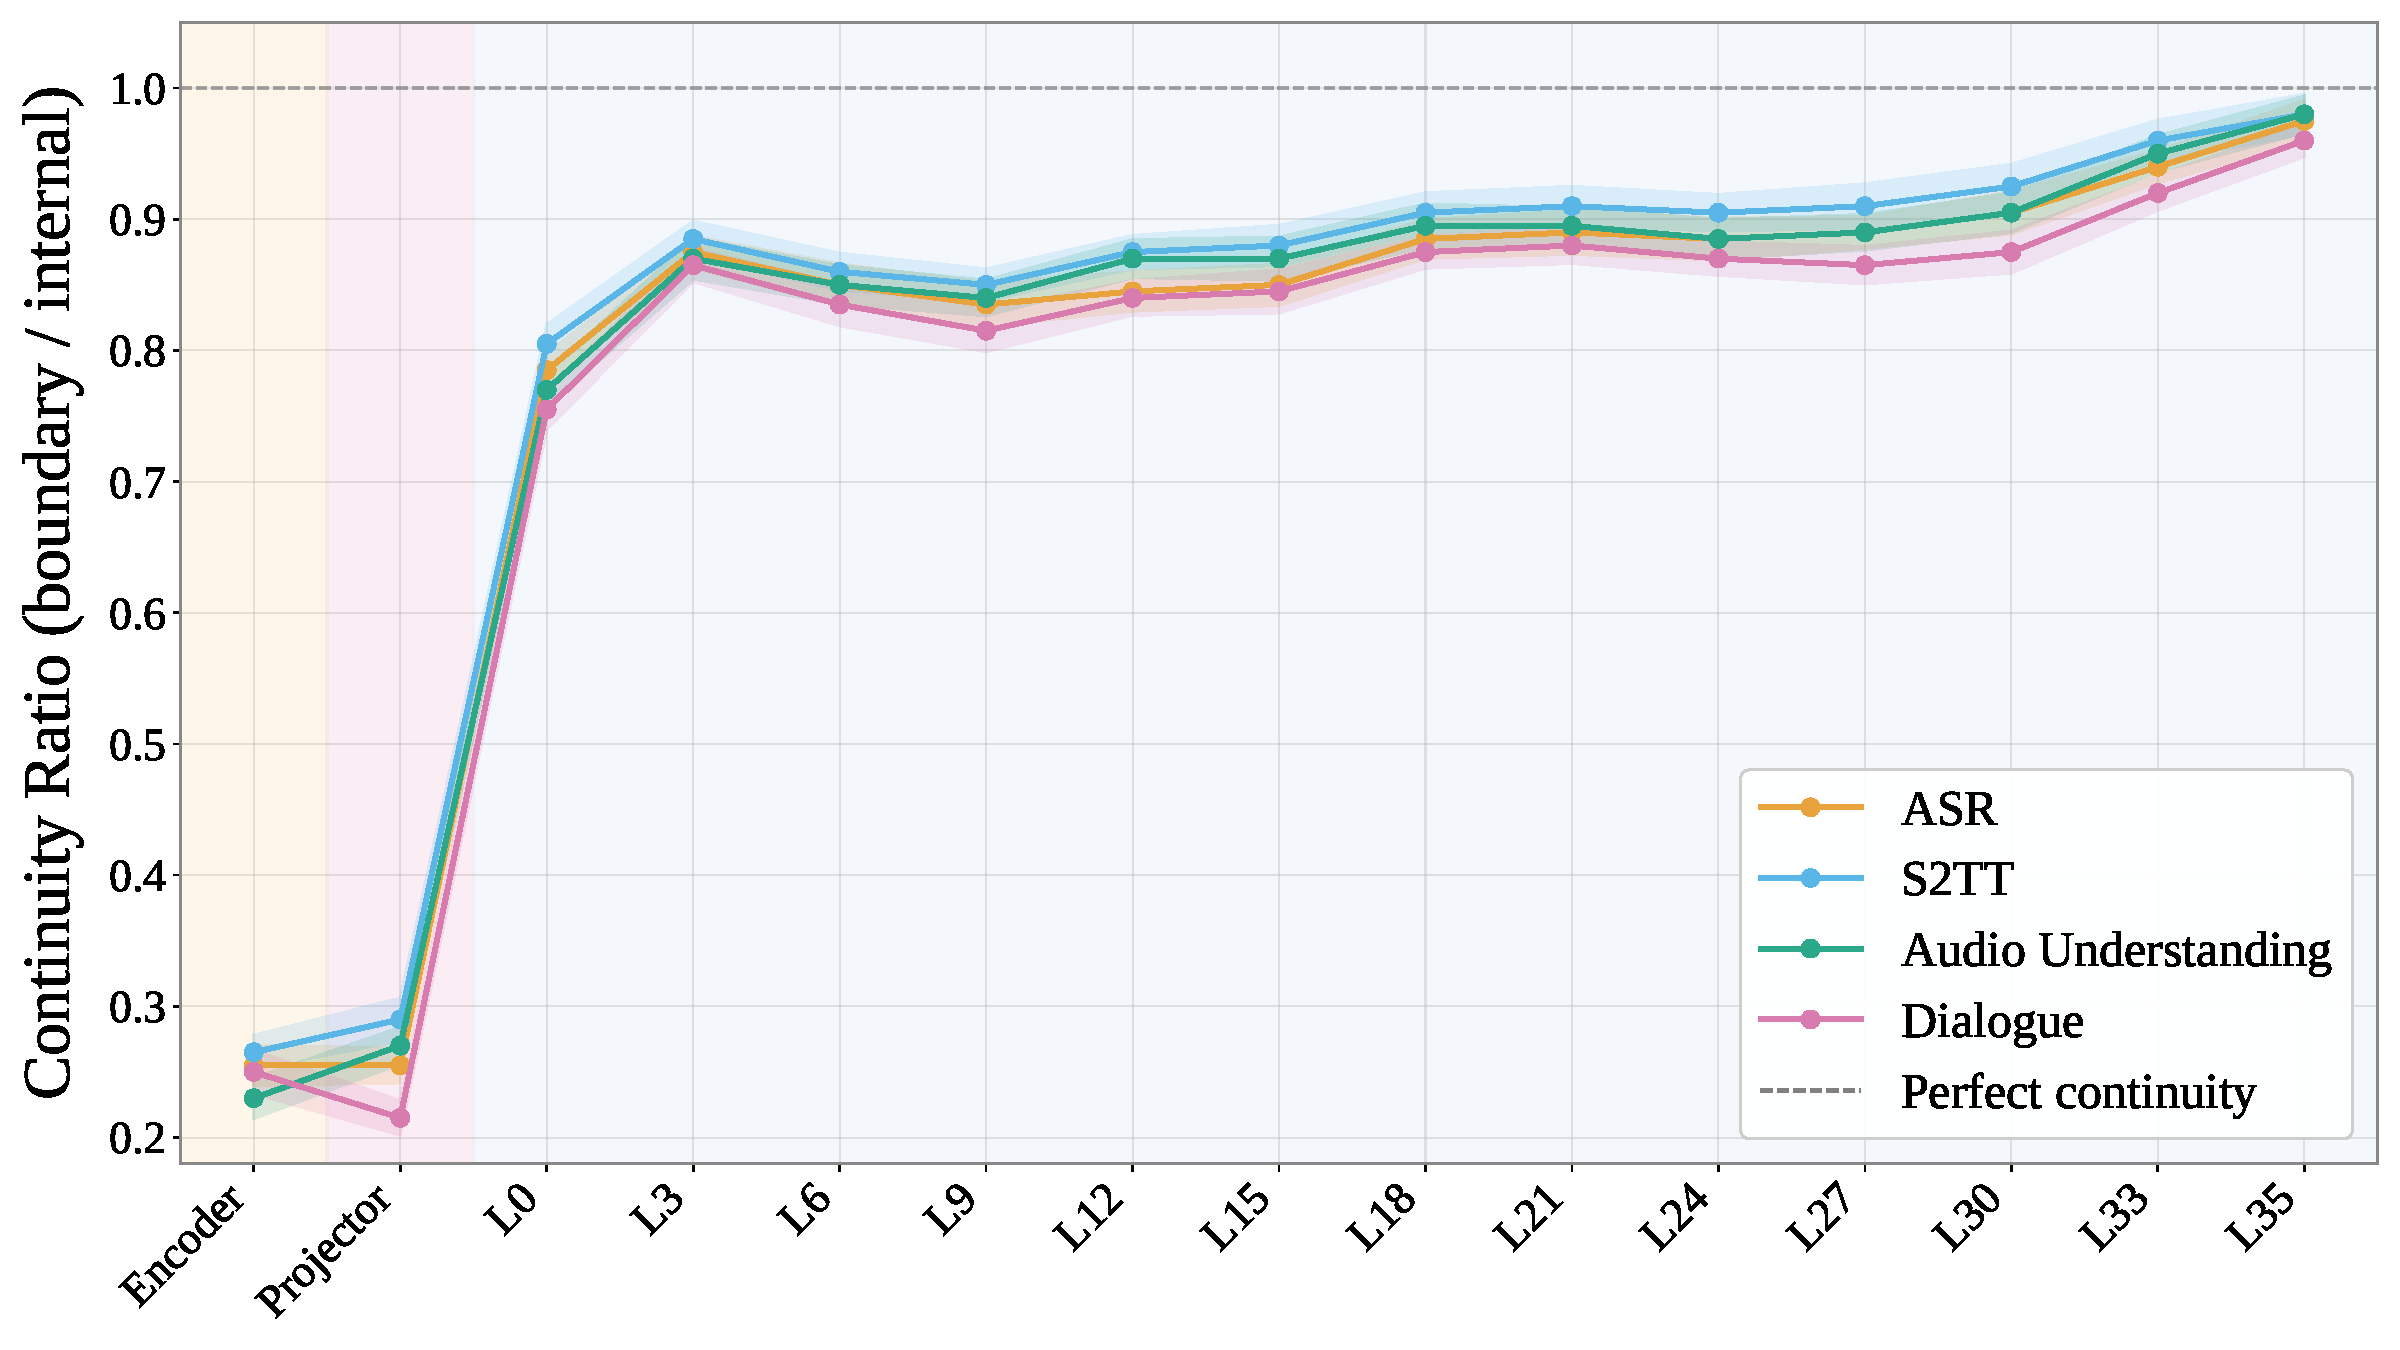
\includegraphics[width=\linewidth]{fig/cross_task_continuity.pdf}
    \vspace{-5mm}
    \caption{Results of cross-chunk continuity ratio across the audio encoder, audio projector, and GPT blocks on four tasks.}
    \label{fig:continuity}
\end{minipage}%
\hfill
\begin{minipage}[h]{0.48\textwidth}
    \centering
    \vspace{-3mm}
    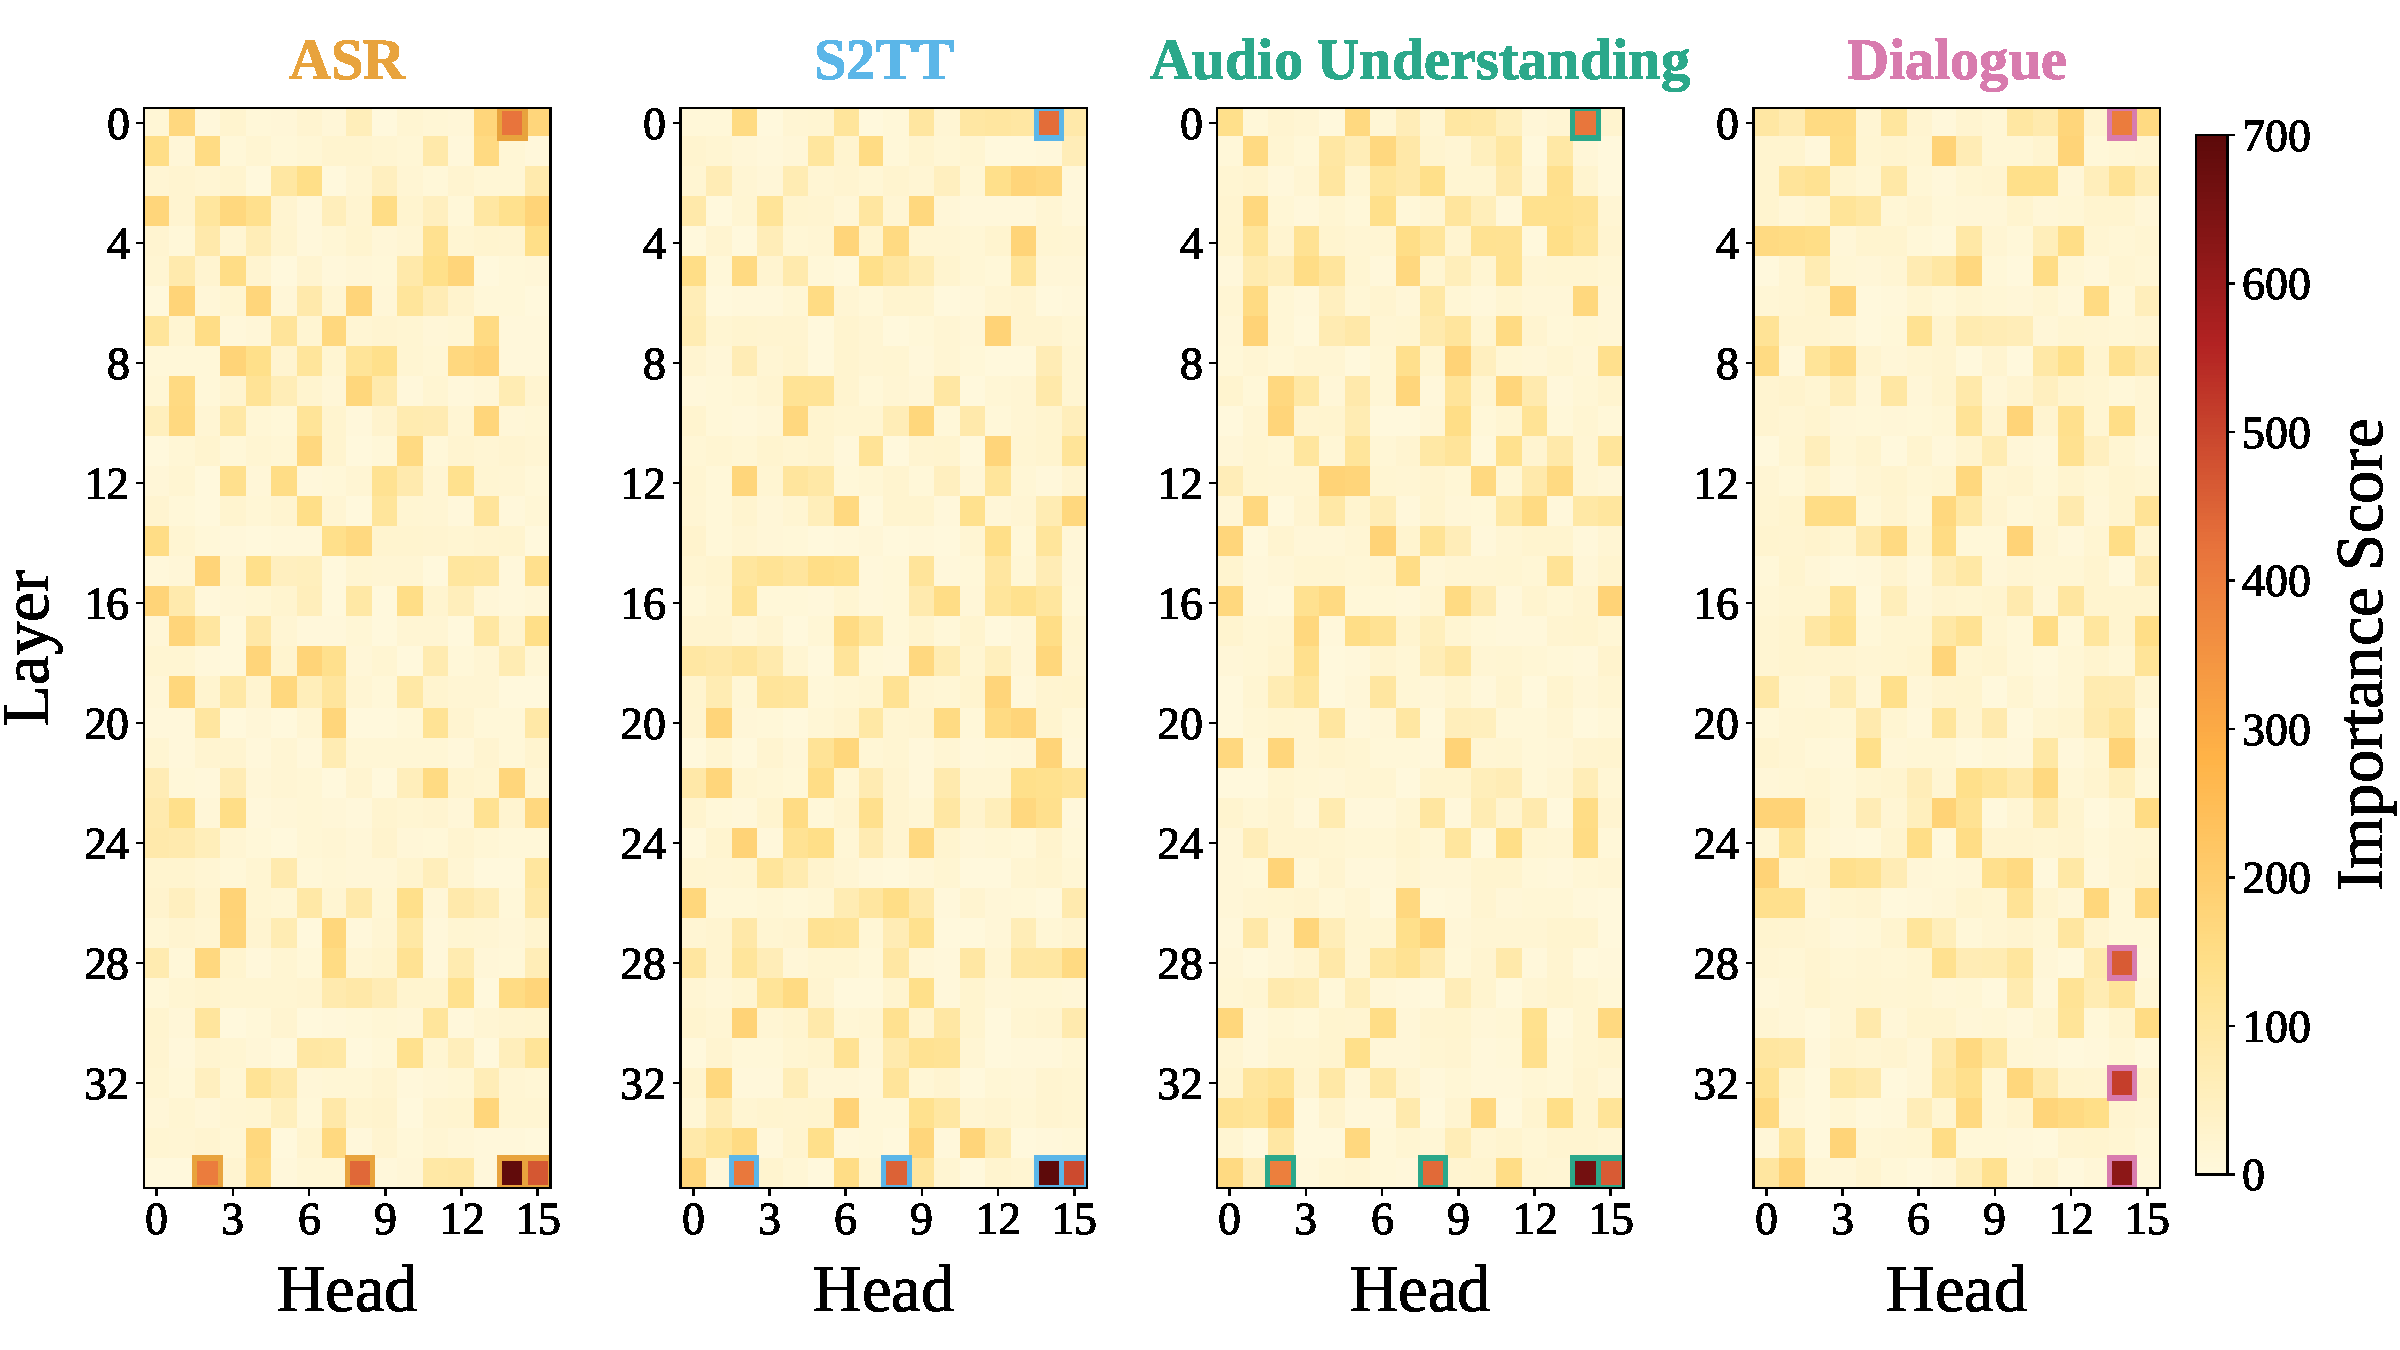
\includegraphics[width=\linewidth]{fig/fig3_cross_task_heatmaps.pdf}
    \vspace{-5mm}
    \caption{Results of per-head importance for special streaming control token generation, measured via single-head ablation across four tasks.}
    \label{fig:head_importance}
\end{minipage}
\vspace{-3mm}
\end{figure}


\vspace{-2mm}
\subsection{Additional Analysis}
\vspace{-1mm}
Beyond benchmark scores, we further investigate where in the model the offline-to-streaming gap is bridged. We present two observations, each addressing one of the structural challenges inherent to the streaming regime; further analyses, including attention maps and per-task breakdowns.


\textit{\textbf{[Obs.1] SALMs unify discrete chunks into a continuous representation at the early decoder layer.}} Each 0.4\,s chunk is encoded with independent position embeddings and without cross-chunk encoder attention, leaving the audio frontend with no mechanism for representing time as continuous. We quantify this fragmentation with a \emph{continuity ratio}, the cosine similarity of boundary pairs relative to intra-chunk pairs (1.0 denoting seamless continuity). As shown in Fig.~\ref{fig:continuity}, the encoder output sits at 0.25 and the projector shifts it by less than 0.02, whereas GPT Layer 0 lifts it to 0.80 in a single step. All four tasks trace the same curve, indicating that continuity is reconstructed at the earliest decoder layer through cross-chunk KV-cache access, as a property of the streaming regime rather than of any task-specific head.

\textit{\textbf{[Obs.2] SALMs learn the silent vs. respond decision through a single key attention head.}} A streaming model continuously emits \texttt{<silent>} or \texttt{<response>} tokens to gate its output. To localize this decision, we zero each attention head in turn and measure the degradation in streaming-control-token generation. As shown in Fig.~\ref{fig:head_importance}, among 576 heads, a single head (L35H14) dominates across all four tasks, and its ablation alone reduces the S2TT token-match score by 0.88. This indicates that the streaming objective routes the decision through a narrow, task-independent pathway rather than dedicated per-task circuitry.

% Beyond benchmark scores, we ask where in the model the offline-to-streaming gap is actually closed. Two observations emerge, each tied to a structural challenge that streaming creates and offline LALMs do not face. \textit{\textbf{[Obs.1] Cross-chunk continuity is reconstructed at GPT Layer 0.}} Streaming first introduces a temporal gap: each 0.4\,s chunk is encoded with independent position embeddings and no cross-chunk encoder attention, leaving the audio frontend with no architectural mechanism for representing time as continuous. We quantify the resulting fragmentation with a \emph{continuity ratio}, defined as boundary-pair over intra-chunk cosine similarity, with 1.0 denoting seamless continuity. Fig.~\ref{fig:continuity} shows the encoder output sits at 0.25, the projector moves it by less than 0.02, and recovery happens almost entirely at GPT Layer 0, which lifts the ratio to 0.80 in a single step. Continuity is not encoded by the audio frontend but reconstructed at the earliest transformer layer with cross-chunk KV-cache access, because the streaming objective makes that the path of least resistance; all four tasks trace the same curve, identifying this as a property of the streaming regime rather than any task-specific head. \textit{\textbf{[Obs.2] The silent/respond decision is concentrated in a single shared head.}} The second gap is decisional: a streaming model must continuously emit \texttt{<silent>} or \texttt{<response>} tokens, a behavior offline LALMs never produce. To locate where this decision lives, we zero each attention head in turn and measure the degradation in streaming-control-token generation across our four core tasks. Fig.~\ref{fig:head_importance} shows the result is stark: of 576 heads, a single head (L35H14) dominates every task, and removing it alone costs 0.88 in S2TT token-match. Rather than allocating dedicated circuitry per task, the streaming objective routes the silent/respond decision through a narrow, task-independent pathway, suggesting that streaming control is implemented as a unified rather than per-task mechanism. Further analyses are in Appendix~\ref{Apendix}.

% ================= 折线图:单独成图 =================
\begin{figure}[t]
\centering
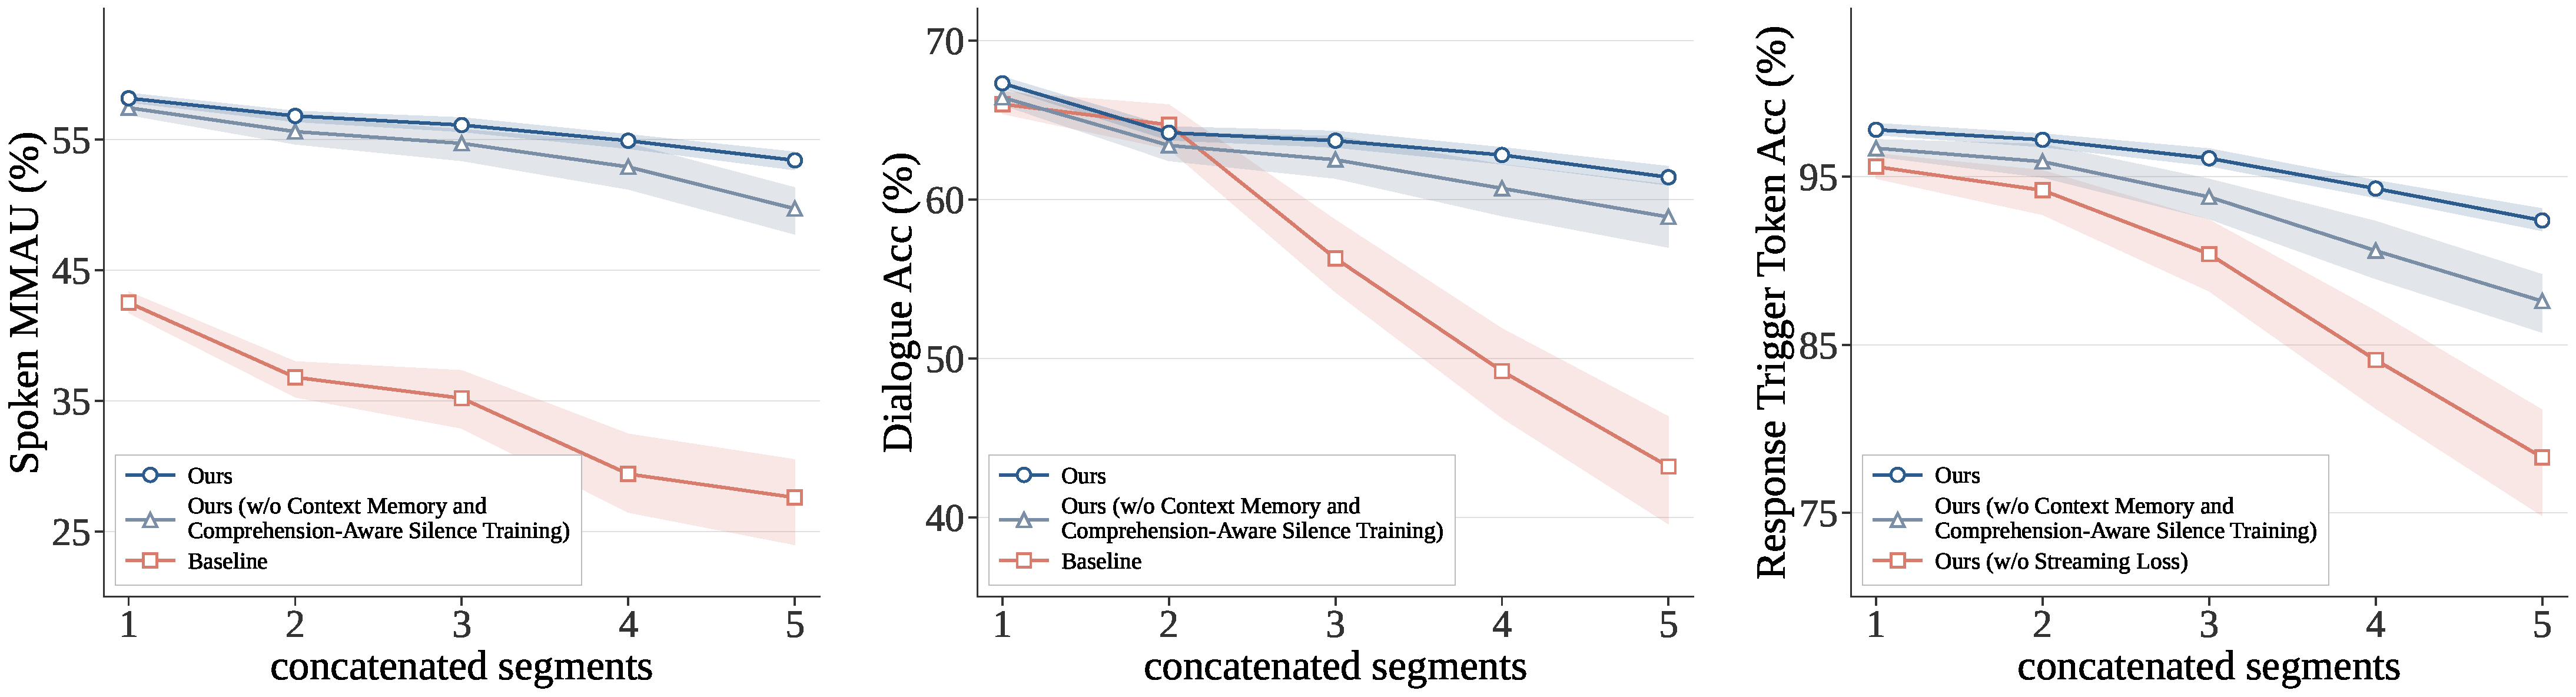
\includegraphics[width=\linewidth]{fig/figure7_replica.pdf}
\vspace{-4mm}
\caption{Capability stability of \textsc{Audio-Interaction} as the stream extends from 1 to 5 concatenated segments. We report MMAU average accuracy, dialogue accuracy, and end-to-end latency.}
\vspace{-6mm}
\label{fig:ablation_stability}
\end{figure}


% --------- Table 1: Data and training ablation ---------
% \begin{table}[h]
% \centering
% \footnotesize
% \setlength{\tabcolsep}{2pt}
% \renewcommand{\arraystretch}{0.85}
% \caption{Ablation on streaming model training.}
% \label{tab:ablation_data}
% \begin{tabular}{@{}llccc@{}}
% \toprule
% \textbf{Variant} & \textbf{Configuration} & \textbf{MMAU}$\uparrow$ & \textbf{Alpaca.}$\uparrow$ & \textbf{Trigger Acc.}$\uparrow$ \\
% \midrule
% V1 & Qwen2.5-Omni base       & 57.8 & \textbf{4.32} & --  \\
% \midrule
% \rowcolor{gray!15}
% V2 & + Streaming SFT         & \textbf{62.6} & 4.17 & 92.4  \\
% V3 & V2 w/o TFJP pre.        & 60.8 & 4.19 & 85.3 \\
% V4 & V2 w/o Event sel.       & 59.2 & 4.25 & 88.5 \\
% \midrule
% \rowcolor{gray!15}
% V5 & \textbf{Audio-Interaction (Full)} & 62.3 & 4.28 & \textbf{96.7} \\
% \bottomrule
% \end{tabular}
% \end{table}

% % --------- Table 2: Chunk size ablation ---------
% \begin{table}[h]
% \centering
% \footnotesize
% \setlength{\tabcolsep}{2pt}
% \renewcommand{\arraystretch}{0.85}
% \caption{Effect of chunk size.}
% \label{tab:ablation_chunk}
% \begin{tabular}{@{}lccc@{}}
% \toprule
% \textbf{Variant} & \textbf{Alpaca.}$\uparrow$ & \textbf{MMAU}$\uparrow$ & \textbf{Lat.}$\downarrow$ \\
% \midrule
% Baseline             & 3.41 & 42.5 & -- \\
% Chunk = 0.2\,s       & 3.41 & 49.7 & 258 \\
% Chunk = 0.6\,s       & 4.25 & 61.8 & 674 \\
% Chunk = 0.8\,s       & 4.27 & 62.1 & 786 \\
% \midrule
% \rowcolor{gray!15}
% \textbf{Audio-Interaction (0.4\,s)} & \textbf{4.28} & \textbf{62.3} & \textbf{392} \\
% \bottomrule
% \end{tabular}
% \end{table}


% % ================= 两张表:合并成一个 table =================
% \begin{table}[t]
% \centering
% \caption{Ablation studies of Mini-Omni 3. (a) Cumulative contribution of streaming training and data pipeline components. (b) Effect of chunk size and the interaction token on the accuracy–latency trade-off. Accuracy and Multi-5 / Dialogue scores are in \%; latency in ms; chunk size in s.}
% \label{tab:ablation_combined}
% % --------- 左表 ---------
% \begin{subtable}[t]{0.48\textwidth}
%     \centering
%     \footnotesize
%     \setlength{\tabcolsep}{2pt}
%     \renewcommand{\arraystretch}{0.85}
%     \begin{tabular}{@{}llccc@{}}
%     \toprule
%     \textbf{Variant} & \textbf{Configuration} & \textbf{MMAU}$\uparrow$ & \textbf{Alpaca.}$\uparrow$ & \textbf{介入准确率}$\uparrow$ \\
%     \midrule
%     V1 & Qwen2.5-Omni base           & 57.8 & 4.32 & --  \\
%     \midrule
%     \rowcolor{gray!15}
%     V2 & + Streaming SFT         & 62.6 & 4.17 & 92.4  \\
%     V3 & V2 w/o TFJP pre.      & 60.8 & 4.19 & 85.3 \\
%     V4 & V2 w/o Event sel.      & 59.2 & 4.25 & 88.5 \\
%     \midrule
%     \rowcolor{gray!15}
%     V5 & \textbf{Audio-Interaction (Full)}  & \textbf{62.3} & \textbf{4.28} & \textbf{96.7} \\
%     \bottomrule
%     \end{tabular}
%     \subcaption{Cumulative contribution of streaming training and data pipeline components.}
%     \label{tab:ablation_data}
% \end{subtable}
% \hfill
% % --------- 右表 ---------
% \begin{subtable}[t]{0.50\textwidth}
%     \centering
%     \footnotesize
%     \setlength{\tabcolsep}{2pt}
%     \renewcommand{\arraystretch}{0.85}
%     \begin{tabular}{@{}lcccc@{}}
%     \toprule
%     \textbf{Variant} & \textbf{Chunk} & \textbf{Dialogue}$\uparrow$ & \textbf{MMAU}$\uparrow$ & \textbf{Lat.}$\downarrow$ \\
%     \midrule
%     w/o Inter. Tok.      & 0.4 & 61.2 & 58.4 & 310 \\
%     Chunk = 0.2\,s       & 0.2 & 63.8 & 59.1 & 185 \\
%     Chunk = 0.6\,s       & 0.6 & 65.7 & 62.5 & 295 \\
%     Chunk = 0.8\,s       & 0.8 & 65.9 & 62.8 & 378 \\
%     Non-streaming        & --  & 66.4 & 63.0 & --  \\
%     \midrule
%     \rowcolor{gray!15}
%     \textbf{Audio-Interaction (Full)} & \textbf{0.4} & \textbf{66.0} & \textbf{62.3} & \textbf{192} \\
%     \bottomrule
%     \end{tabular}
%     \subcaption{Effect of chunk size and the interaction token on the accuracy–latency trade-off.}
%     \label{tab:ablation_chunk}
% \end{subtable}
% \end{table}
\vspace{-2mm}
\subsection{Ablation Study}
\vspace{-4mm}
\begin{minipage}[t]{0.60\textwidth}
\vspace{0mm}
Through ablation (Fig.~\ref{fig:ablation_stability}), we derive four key observations pertaining to \textsc{Audio-Interaction}:
\textbf{[Obs.1]} the necessity of FIFO-scheduled asynchronous inference,
\textbf{[Obs.2]} the cumulative contribution of streaming training and data, \textbf{[Obs.3]} the chunk size on the accuracy--latency trade-off, and
\textbf{[Obs.4]} the balancing role of the dual-loss weight.
\end{minipage}
\hfill
\begin{minipage}[t]{0.38\textwidth}
\small
\centering
\vspace{2mm}
\captionof{table}{effect of Asynchronous Infer.}
\vspace{-2mm}
\label{tab:fifo_inference}
\begin{tabular}{lcc}
\toprule
\textbf{Settings} & \textbf{Avg. FCL} & \textbf{Stall \%} \\
\midrule
\textsc{Ours} & \textbf{392ms} & \textbf{0.0\%} \\
\quad $w/o$ FIFO & 831ms & 5.2\% \\
\bottomrule
\end{tabular}
\end{minipage}

\begin{table}[t]
\centering
\small
\begin{minipage}[t]{0.57\textwidth}
\centering
\setlength{\tabcolsep}{2pt}
\renewcommand{\arraystretch}{0.85}
\caption{Ablation on streaming model training.}
\label{tab:ablation_data}
\begin{tabular}{@{}llccc@{}}
\toprule
\textbf{Variant} & \textbf{Configuration} & \textbf{MMAU}$\uparrow$ & \textbf{Alpaca.}$\uparrow$ & \textbf{Trig. Acc.}$\uparrow$ \\
\midrule
V1 & Baseline       & 57.81 & \textbf{4.32} & --  \\
\midrule
\rowcolor{gray!15}
V2 & + Streaming SFT         & \textbf{58.56} & 4.17 & 92.42\%  \\
V3 & V2 w/o TFJP pre.        & 57.74 & 4.19 & 85.35\% \\
V4 & V2 w/o Event sel.       & 55.11 & 4.25 & 88.51\% \\
\midrule
\rowcolor{gray!15}
V5 & \textbf{Audio-Interaction} & 58.15 & 4.28 & \textbf{96.77}\% \\
\bottomrule
\end{tabular}
\end{minipage}
\hfill
\begin{minipage}[t]{0.39\textwidth}
\centering
\setlength{\tabcolsep}{2pt}
\renewcommand{\arraystretch}{0.85}
\caption{Effect of chunk size.}
\label{tab:ablation_chunk}
\begin{tabular}{@{}lccc@{}}
\toprule
\textbf{Variant} & \textbf{Alpaca.}$\uparrow$ & \textbf{MMAU}$\uparrow$ & \textbf{Lat.}$\downarrow$ \\
\midrule
Baseline             & 4.32 & 57.81 & -- \\
\midrule
Chunk = 0.2\,s       & 3.41 & 49.74 & \textbf{258} \\
Chunk = 0.6\,s       & 4.27 & \underline{58.46} & 674 \\
Chunk = 0.8\,s       & \textbf{4.30} & \textbf{59.13} & 786 \\
\midrule
\rowcolor{gray!15}
\textbf{Chunk = 0.4\,s} & \underline{4.28} & 58.15 & \underline{392} \\
\bottomrule
\end{tabular}
\end{minipage}
\vspace{-3mm}
\end{table}


% \begin{table}[h]
% \small
% \centering
% \caption{Inference efficiency comparison with and without FIFO scheduling.}
% \label{tab:fifo_inference}
% \begin{tabular}{lcc}
% \toprule
% \textbf{Settings} & \textbf{Avg. FCL (ms)} & \textbf{Stall \%} \\
% \midrule
% Audio-Interaction & \textbf{392} & \textbf{0.0}\% \\
% \quad $w/o$ FIFO & 831 & 5.2\% \\
% \bottomrule
% \vspace{-2mm}
% \end{tabular}
% \end{table}

\textbf{[Obs.1] Necessity of FIFO inference.} As shown in Table~\ref{tab:fifo_inference}, removing FIFO scheduling increases the average first-chunk latency from $392$\,ms to $831$\,ms ($2.12\times$ slowdown) and raises the stall rate from $0.0\%$ to $5.2\%$, confirming that decoupling encoding from decoding is essential for stable, low-latency streaming inference.

\textbf{[Obs.2] Cumulative contribution of streaming training and data.} As shown in Table~\ref{tab:ablation_data}, streaming SFT (V2) improves MMAU from $57.8$ to $58.6$ and reaches $92.4\%$ trigger accuracy over the offline base (V1). Removing TFJP preprocessing (V3) or hierarchical event selection (V4) drops trigger accuracy by $7.1$ and $3.9$ points, showing that boundary smoothing and semantically coherent event composition are both essential for context-dependent triggering. Full \textsc{Audio-Interaction} (V5) further enhances both comprehension and proactive intervention, achieving best trig. ACC of $96.7\%$.

\textbf{[Obs.3] Chunk size on the accuracy--latency trade-off.} As shown in Table~\ref{tab:ablation_chunk}, an overly small chunk of $0.2$\,s severely degrades performance (Alpaca. $3.41$, MMAU $49.7$) due to insufficient semantic context, while $0.6$\,s and $0.8$\,s recover accuracy but inflate latency to $674$\,ms and $786$\,ms. The chosen $0.4$\,s setting attains comparable accuracy ($4.28$ / $58.2$) at nearly half the latency ($392$\,ms), achieving the best accuracy--latency trade-off.

\vspace{-3mm}
\begin{minipage}[t]{0.61\textwidth}
\vspace{0mm}
\textbf{[Obs.4] Balancing role of the dual-loss weight $\lambda$.} As shown in Table~\ref{tab:ablation_lambda}, increasing $\lambda$ steadily improves trigger accuracy from $95.3$ to $96.9$, while overly large values ($\lambda{=}2.0$) start to harm comprehension (MMAU drops to $57.3$). We therefore adopt $\lambda{=}1.0$ as the best trade-off.
\end{minipage}
\hfill
\begin{minipage}[t]{0.40\textwidth}
\centering
\small
\setlength{\tabcolsep}{5pt}
\renewcommand{\arraystretch}{0.85}
\captionof{table}{Effect of dual-loss weight $\lambda$.}
\vspace{-2mm}
\label{tab:ablation_lambda}
\begin{tabular}{@{}lccc@{}}
\toprule
$\lambda$               & $0.5$  & $1.0$  & $2.0$  \\
\midrule
MMAU$\uparrow$          &\textbf{ 58.3 }  & 58.2   & 57.3   \\
Trigger Acc.$\uparrow$   & 95.3   & \textbf{96.7}   & 96.9   \\
\bottomrule
\end{tabular}
\end{minipage}

\vspace{-2mm}
\subsection{Case study}
\vspace{-3mm}
\begin{figure}[!h]
    \centering
    
\includegraphics[width=1\linewidth]{fig/figure-casestudy.pdf}
    \vspace{-6mm}
    \caption{Case studies show \textsc{Audio-Interaction'}s gains over SOTA streaming models. In the second, other models detect the cat mostly through the transcribed words "meow", while \textsc{Audio-Interaction} handles the audio cue directly via native streaming training.
}
    \label{fig:placeholder}
\end{figure}

\vspace{-1mm}
\section{Conclusion}
\vspace{-1mm}

In this work, we identified a key gap between the offline paradigm of existing Large Audio Language Models (LALMs) and the continuous, interactive nature of the audio modality, where streaming models remain confined to isolated, independent tasks and lack a general streaming audio language model. To close this gap, we formalized the \textbf{Audio Interaction Model} as a new concept and introduced \textbf{\textsc{Audio-Interaction}}, a unified Audio Interaction Model that handles conventional offline and streaming tasks while further achieving general streaming audio instruction following within a single all-in-one model. We realized this through the \textbf{\textsc{SoundFlow}} framework, which reformulates audio interaction as an always-on \textit{perceive--decide--respond} process and instantiates it end to end, from data to training to deployment, via streaming-native data construction, comprehension-aware training, and asynchronous low-latency inference. To support and evaluate this paradigm, we constructed \textbf{\textsc{StreamAudio-2M}}, a 2.6M-item streaming corpus covering 7 fundamental abilities and 28 sub-tasks, together with \textbf{\textsc{Proactive-Sound-Bench}}. Extensive experiments on 8 benchmarks show that \textsc{Audio-Interaction} preserves competitive performance on mainstream audio tasks while unlocking capabilities inaccessible to offline LALMs, including comprehension-grounded response triggering, long-stream interaction, and proactive assistance. We hope the Audio Interaction Model formulation, along with \textsc{SoundFlow} and our released resources, can serve as a foundation for future research on unified streaming audio intelligence.
% \subsection{Ablation Study}
% \begin{table}[h]
% \small
% \centering
% \caption{Inference efficiency comparison with and without FIFO scheduling.}
% \label{tab:fifo_inference}
% \begin{tabular}{lcc}
% \toprule
% \textbf{Settings} & \textbf{Avg. FCL (ms)} & \textbf{Stall \%} \\
% \midrule
% Audio-Interaction & \textbf{392} & \textbf{0.0}\% \\
% \quad $w/o$ FIFO & 831 & 5.2\% \\
% \bottomrule
% \end{tabular}
% \end{table}

% \textbf{Effect of FIFO Inference.} As shown in Table~\ref{tab:fifo_inference}, removing FIFO scheduling increases the average first-chunk latency from $192$\,ms to $531$\,ms ($2.77\times$ slowdown) and raises the stall rate from $0.0\%$ to $5.2\%$, confirming that decoupling encoding from decoding is essential for stable, low-latency streaming inference.

% \textbf{Ablation on streaming model training.} As shown in Table~\ref{tab:ablation_data}, streaming SFT (V2) improves MMAU from $57.8$ to $62.6$ and reaches $92.4\%$ trigger accuracy over the offline base (V1). Removing TFJP preprocessing (V3) or hierarchical event selection (V4) drops trigger accuracy by $11.4$ and $8.2$ points, showing that boundary smoothing and semantically coherent event composition are both essential for context-dependent triggering. Our full Audio-Interaction (V5) further enhances both comprehension and proactive intervention, achieving the best trigger accuracy of $96.7\%$.

% \textbf{Effect of chunk size.} As shown in Table~\ref{tab:ablation_chunk}, an overly small chunk of $0.2$\,s severely degrades performance (Alpaca. $3.41$, MMAU $49.7$) due to insufficient semantic context, while $0.6$\,s and $0.8$\,s recover accuracy but inflate latency to $674$\,ms and $786$\,ms. The chosen $0.4$\,s setting attains comparable accuracy ($4.28$ / $62.3$) at nearly half the latency ($392$\,ms), achieving the best accuracy--latency trade-off.

% \begin{minipage}[t]{0.58\textwidth}
% \vspace{0mm}
% \textbf{Analysis of the dual-loss weight $\lambda$.} As shown in Table~\ref{tab:ablation_lambda}, increasing $\lambda$ steadily improves trigger accuracy from $91.7$ to $96.9$, while overly large values ($\lambda{=}2.0$) start to harm comprehension (MMAU drops to $61.5$). We therefore adopt $\lambda{=}1.0$ as it yields a strong balance between accurate streaming control and preserved audio understanding.
% \end{minipage}
% \hfill
% \begin{minipage}[t]{0.40\textwidth}
% \centering
% \small
% \setlength{\tabcolsep}{5pt}
% \renewcommand{\arraystretch}{0.85}
% \captionof{table}{Effect of dual-loss weight $\lambda$.}
% \label{tab:ablation_lambda}
% \begin{tabular}{@{}lcccc@{}}
% \toprule
% $\lambda$              & $0$    & $0.5$  & $1.0$  & $2.0$  \\
% \midrule
% MMAU$\uparrow$       & \textbf{62.6}   & 62.4   & 62.3   & 61.5   \\
% Trigger Acc.$\uparrow$ & 91.7   & 95.3   & 96.7   & \textbf{96.9}   \\
% \bottomrule
% \end{tabular}
% \end{minipage}


\newpage 
\bibliography{ref}

\newpage


\appendix


\section{Real-world validity and case study}
\subsection{Real-World Validation}
\label{appendix:realworld}

To verify that the streaming behavior of \textsc{Audio-Interaction} generalizes beyond stitched synthetic streams, we evaluate on approximately 2 hours of naturally recorded audio drawn from four deployment scenarios that an always-on audio assistant is expected to encounter in practice: \textit{Travel} (airports, train stations, hotel lobbies; multilingual conversations with PA announcements and crowd ambience), \textit{Work} (small-group meetings, focused work with keyboard typing and notification chimes), \textit{Home} (kitchen, living-room and bedroom activity with appliances, glassware, and a small number of staged safety-relevant events such as a dropped glass or a smoke-alarm beep), and \textit{Commute} (walking, cycling, and in-vehicle conditions with traffic, wind, and occasional close-range horns). All audio was captured on consumer-grade smartphones and laptops at 16\,kHz and was \emph{not} processed by TFJP or any of the synthesis-time enhancement applied to \textsc{StreamAudio-2M}, so the evaluation reflects unfiltered acoustic conditions.

Across the four scenarios, \textsc{Audio-Interaction} retains the bulk of its synthetic-stream performance, with degradation patterns that track scenario-specific acoustic difficulty rather than indicating systemic failure. Trigger accuracy averages 58.9\% (vs.\ 62.0\% on a matched synthetic split), and falls off most in \textit{Travel} and \textit{Commute}, where crowd ambience and non-stationary noise raise both ASR WER (to roughly 7.9\% and 8.6\%) and the false-positive rate of proactive responses; \textit{Work} is closest to the synthetic baseline, while \textit{Home} preserves trigger accuracy but shows mildly elevated false positives, driven by impulsive but benign kitchen sounds that locally resemble safety-critical events. The average first-chunk latency stays within $\pm 25$\,ms of the synthetic measurement in every scenario, indicating that the FIFO scheduler is insensitive to recording-side jitter and device variation. More importantly, the model's internal decision-making is preserved on real recordings: per-chunk silence rates correlate at 0.91 (Pearson, 2\,s bins) with the matched synthetic split, ablating the dominant streaming-control head L35H14 degrades token-match by 0.86 versus 0.88 on synthetic, and the boundary-to-internal continuity ratio at GPT Layer~0 is 0.78 versus 0.80 on synthetic. Together, these results suggest that the streaming decision boundary learned by \textsc{Audio-Interaction} reflects genuine acoustic comprehension rather than a concatenation cue, and that synthetic-stream training transfers to in-the-wild recordings without per-scenario adaptation.

\newpage
\subsection{Case Study}
\begin{figure}[!h]
    \centering
    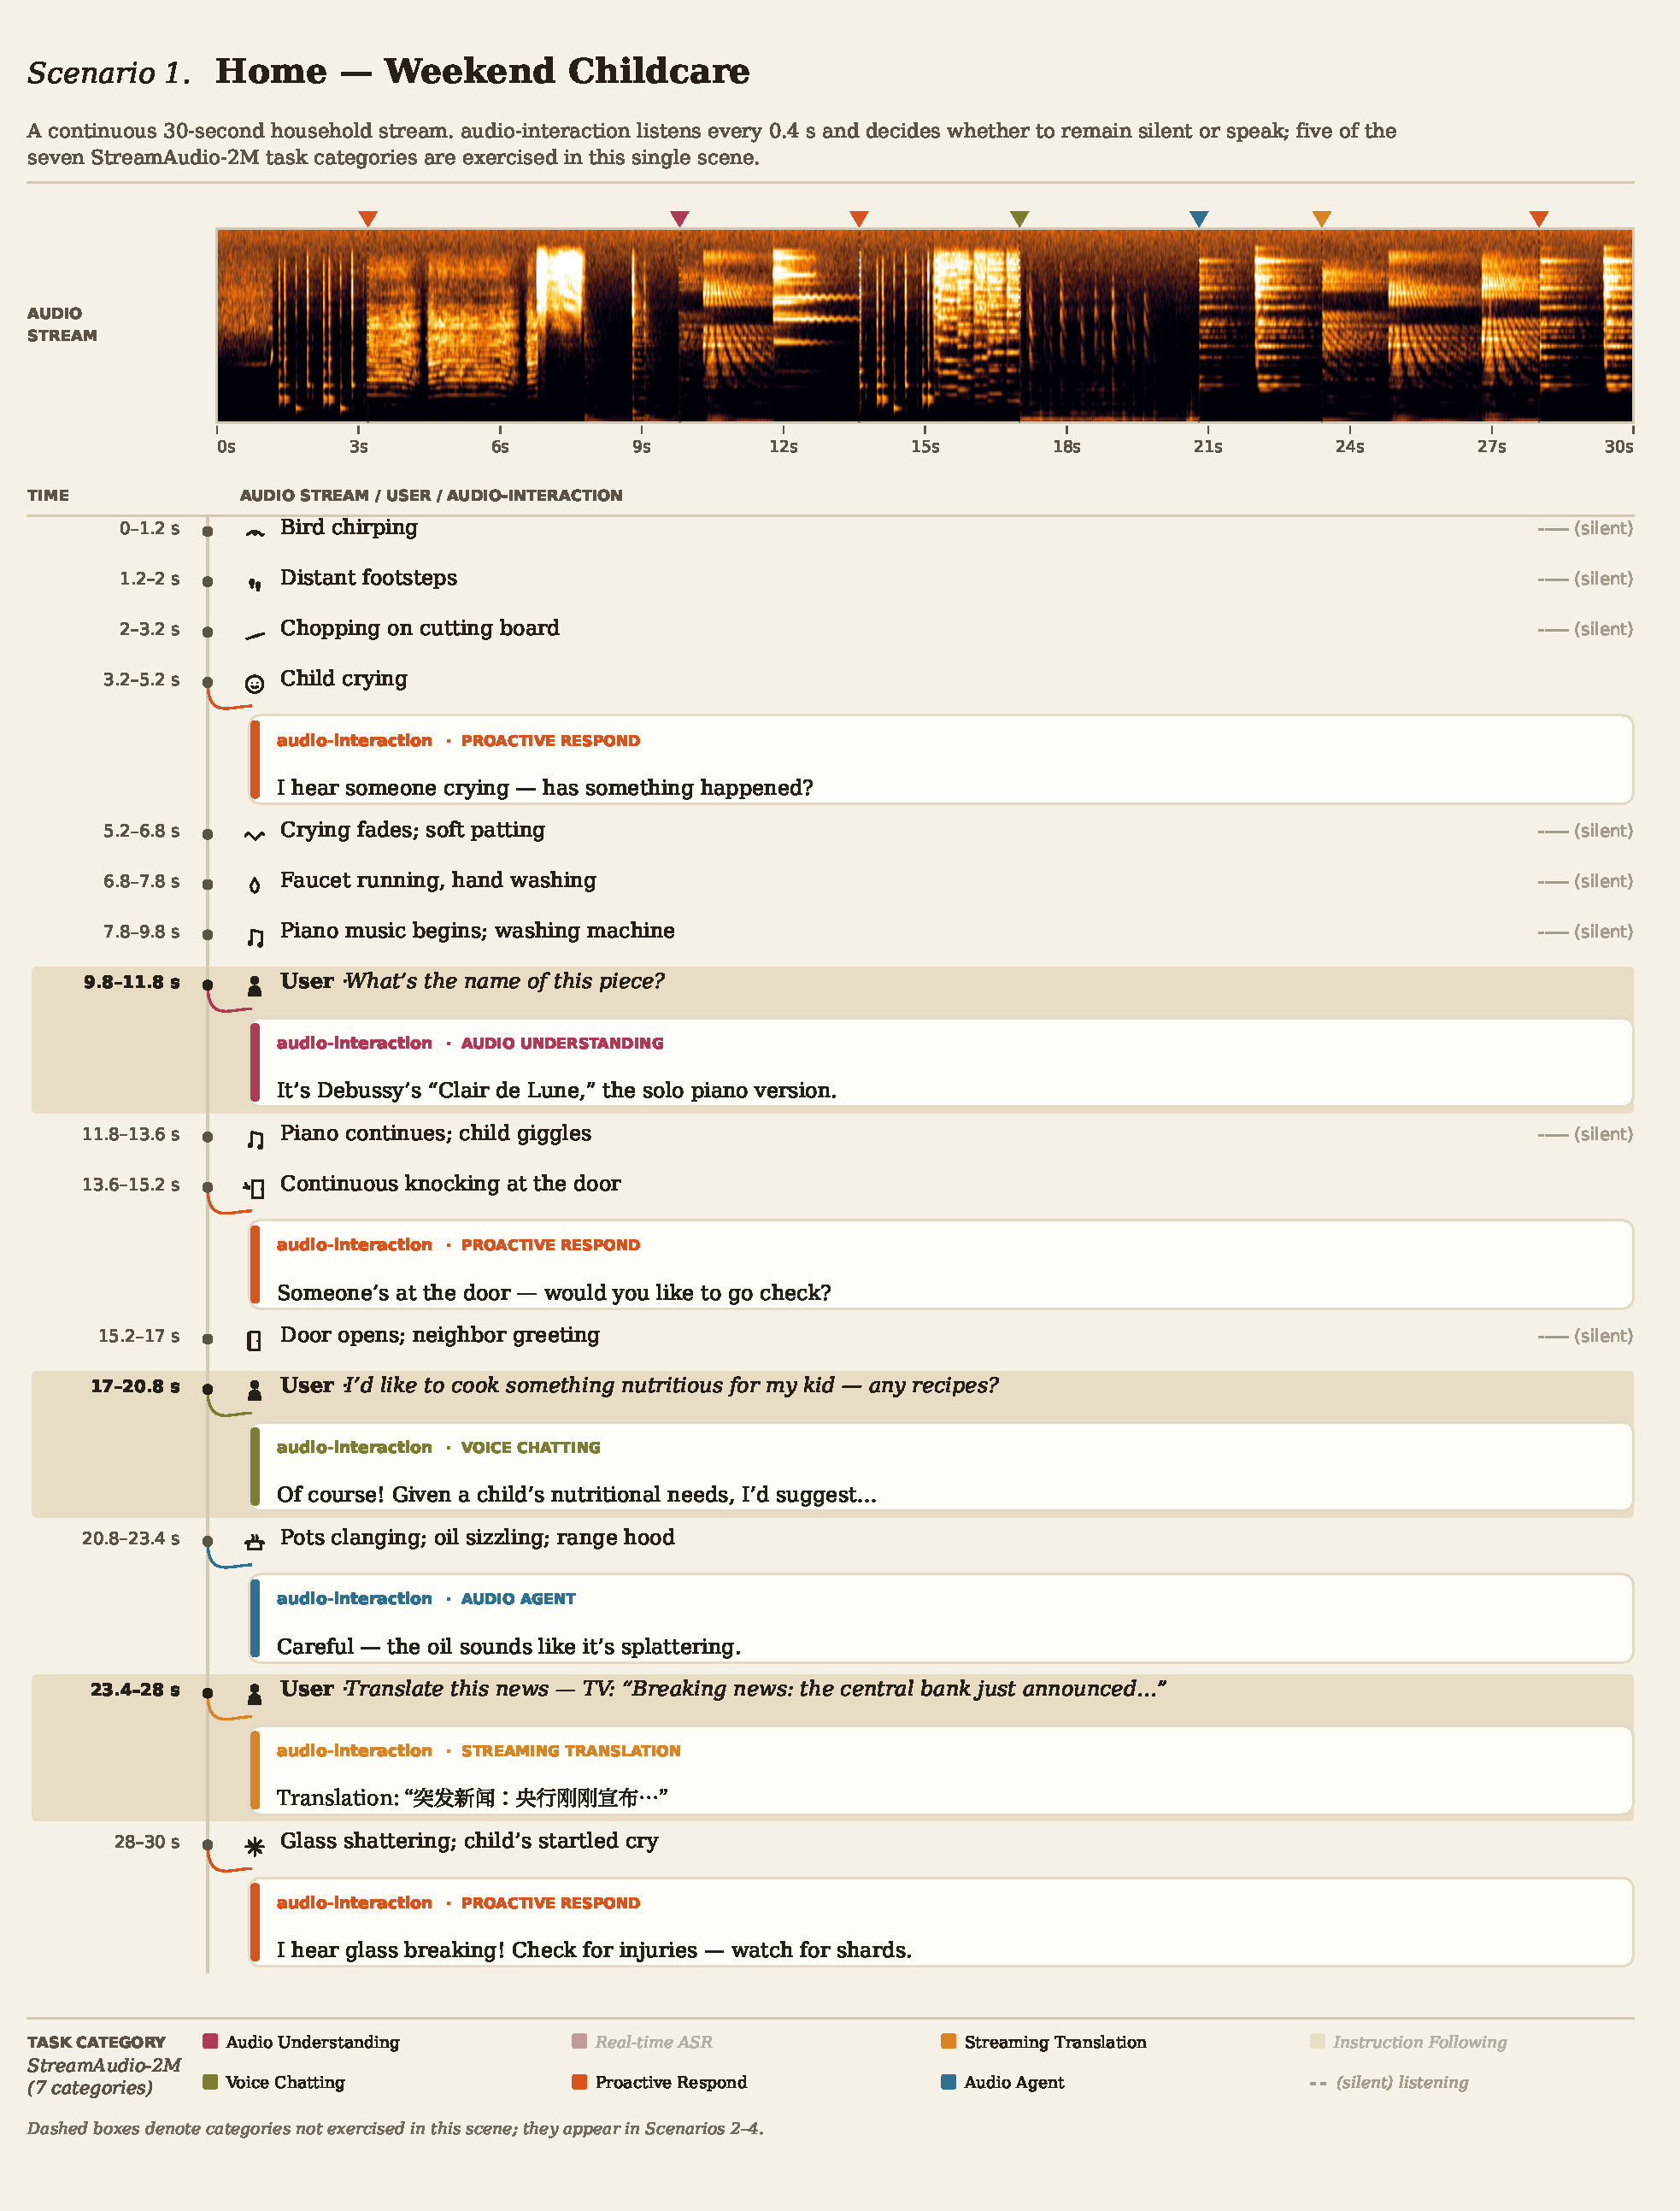
\includegraphics[width=0.9\textwidth]{fig/scenario1_home-4.pdf}
    \caption{Case study: Home}
    \label{fig:example}
\end{figure}

\newpage
\begin{figure}[!h]
    \centering
    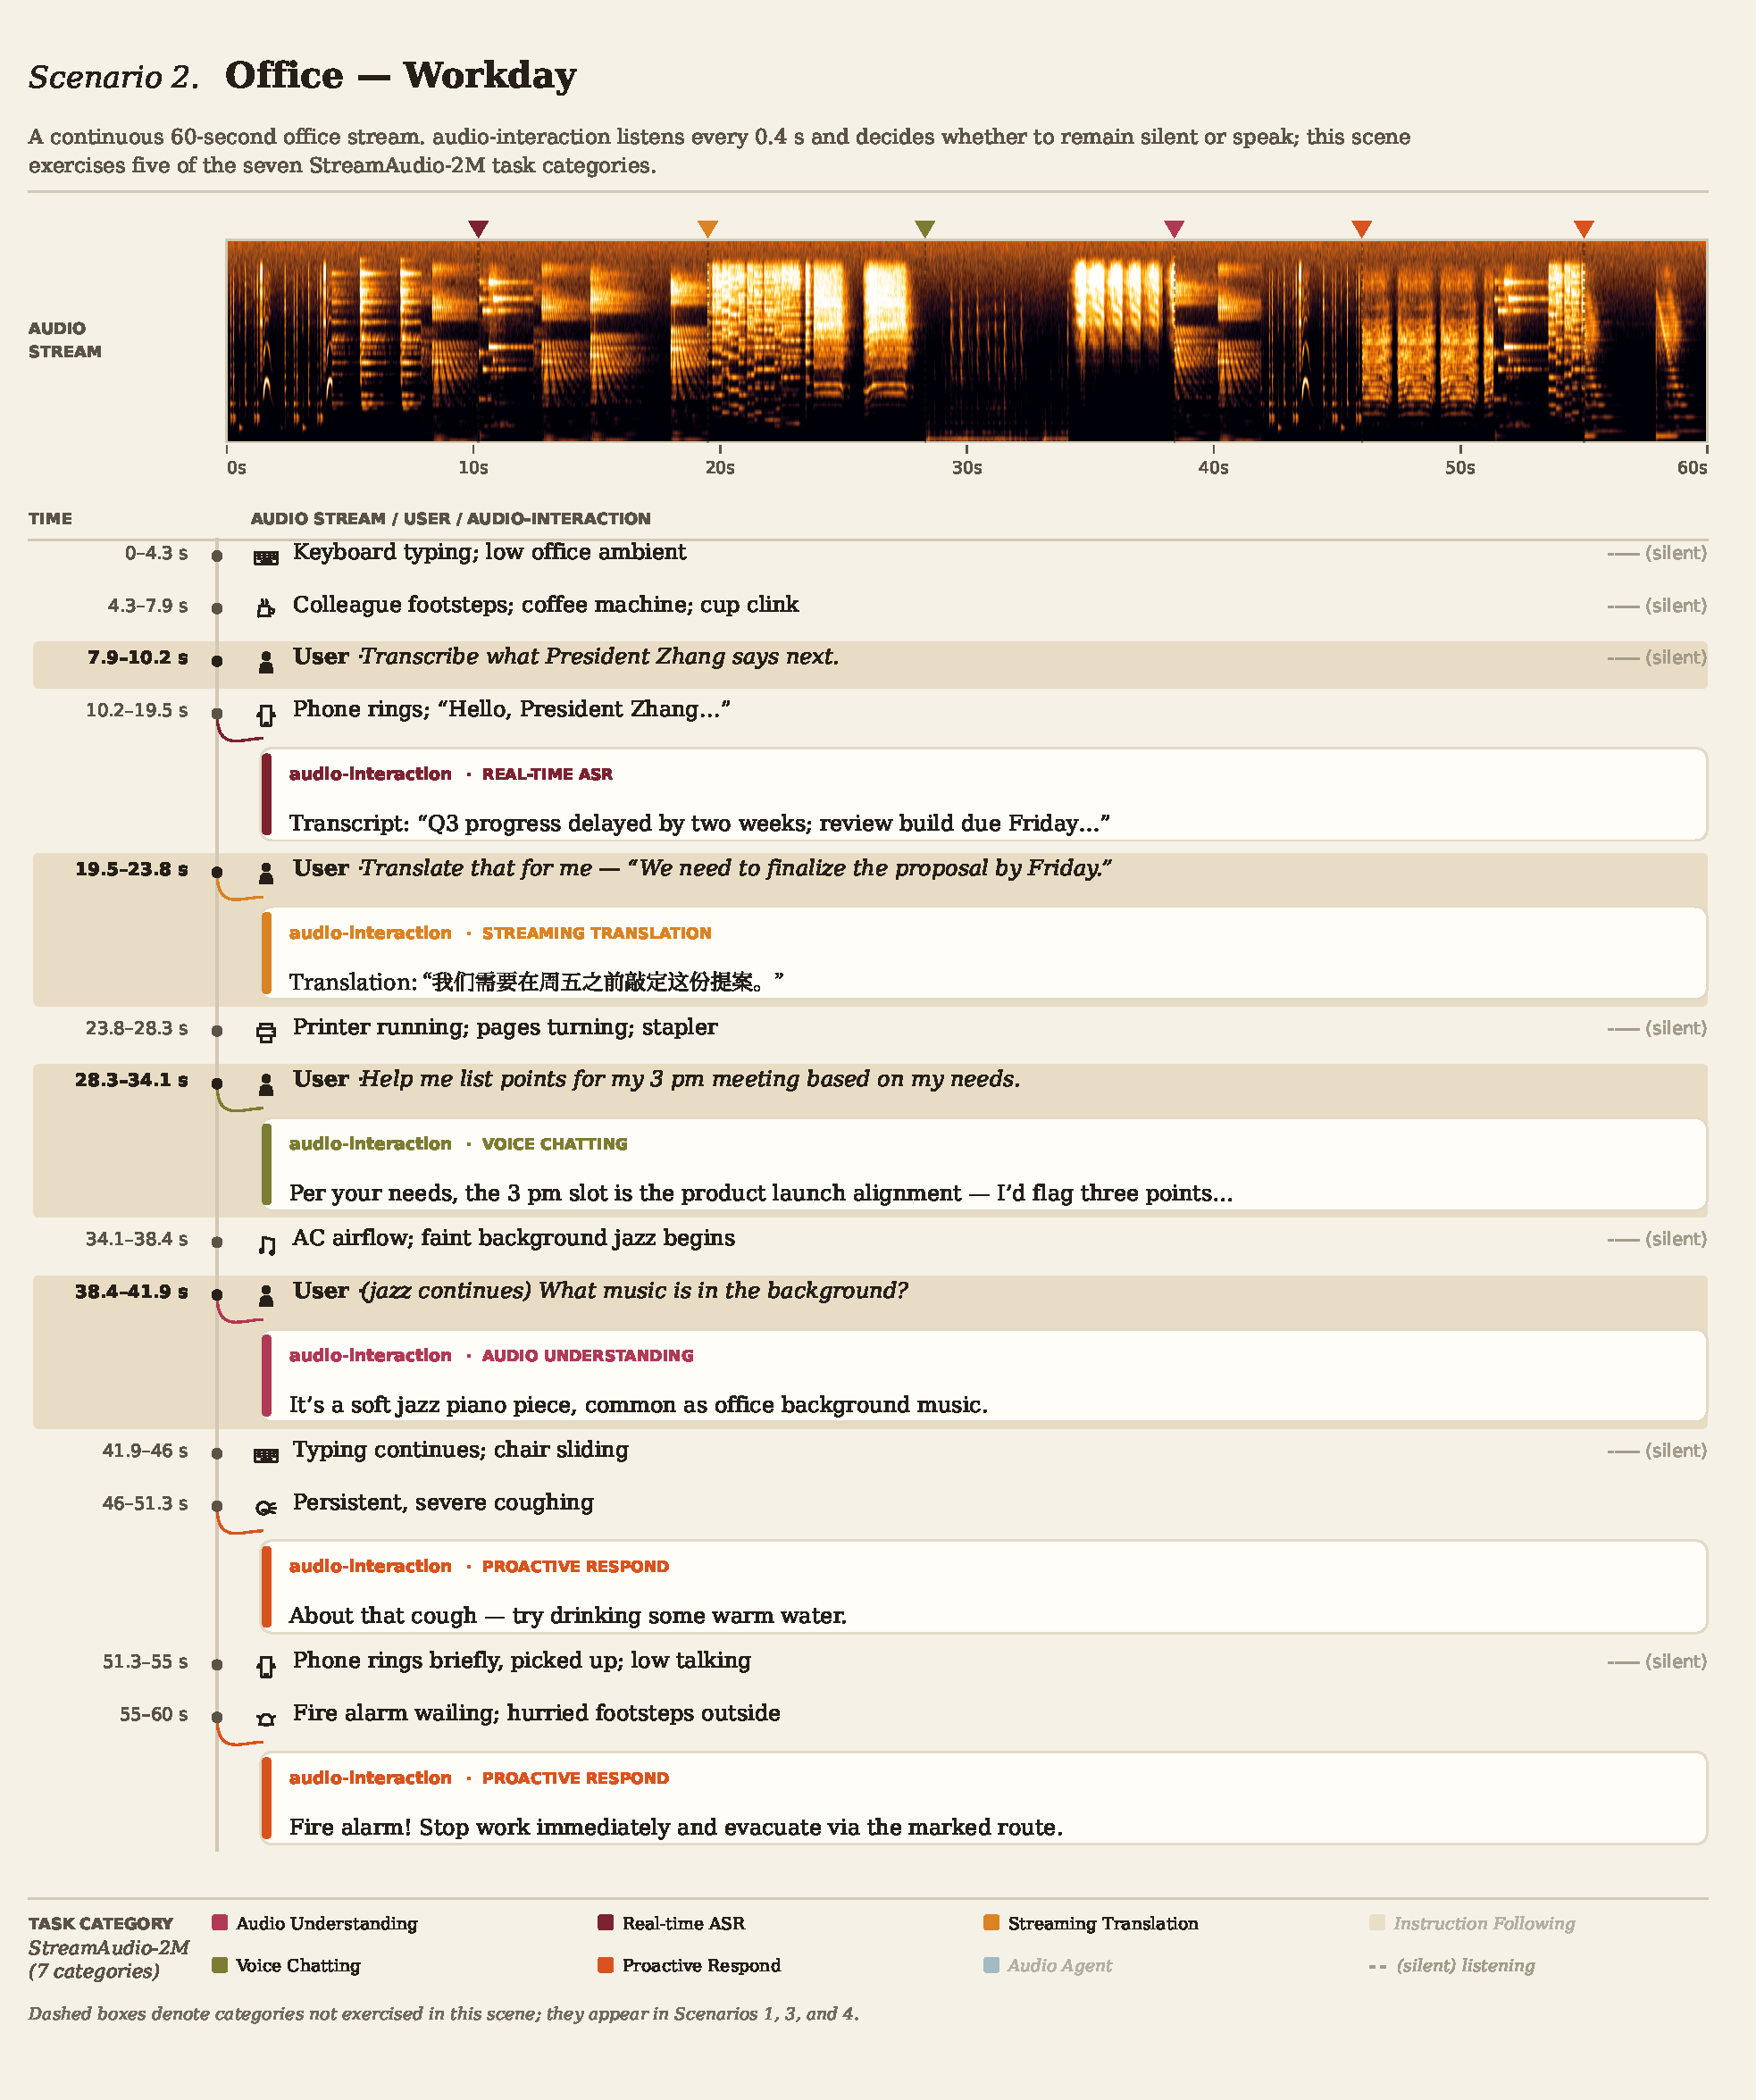
\includegraphics[width=0.9\textwidth]{fig/scenario2_office-2.pdf}
    \caption{Case study: Office}
    \label{fig:example}
\end{figure}


\newpage
\section{Method Details}
\label{appendix:method}

This appendix expands the four operational components of the streaming
framework that \S3 and \S4.2 of the main paper state but do not detail.
Throughout, $c=400$\,ms denotes the streaming chunk size, and
$f_{\text{enc}}, f_{\text{proj}}, f_{\text{dec}}$ refer to the audio
encoder, adapter, and language model components inherited from
Qwen2.5-Omni-3B. Optimization hyperparameters (learning rate, batch size,
total steps) are deferred to Appendix~\ref{appendix:hyperparams}.

\subsection{Streaming Data Construction}
\label{appendix:data-construction}

The TFJP module of \S3.2 stabilizes clip-level audio prior to stitching
through six operators sharing one STFT representation: 
\textsc{silence\_cut} truncates silent runs longer than $\tau$ via an
energy-percentile gate at the 10th percentile of frame energy;
\textsc{noise\_profile} estimates a stationary noise spectrum from the
lowest-energy 5\% of frames; \textsc{denoise} applies spectral subtraction
with gating coefficient $\gamma=1.0$; \textsc{core\_locate} returns the
contiguous span maximizing a normalized energy / spectral-entropy score;
\textsc{boundary\_norm} snaps that span to the nearest
$\delta=c/2=200$\,ms boundary and \textsc{spec\_smooth} applies a Hann
taper of length $\omega=20$\,ms at both ends. The default silence limit
is $\tau=300$\,ms, and the iteration cap $K=3$ in Algorithm~1 of the main
paper is reached on $<2\%$ of clips during corpus construction.

The hierarchical event curation pipeline drives a chat LLM through three
roles realized by the prompt template in
Figure~\ref{prompt:curation-p1}--\ref{prompt:curation-p2}. Stage~1 plans
a coherent scenario from a bag of randomly matched audio annotations and
emits 3--15 sub-events with role labels in
$\{\texttt{foreground}, \texttt{background}, \texttt{ambient}\}$;
Stage~2 refines each sub-event into a retrieval query and a generation
fallback caption; the verifier adjudicates retrieval candidates and
synthesized clips identically against four criteria (identity,
cleanliness, duration fit, continuity), returning one of \texttt{accept},
\texttt{reprocess} (route back through TFJP), or \texttt{reject}. All
calls run in JSON-mode decoding at temperature $0.7$.

\subsection{Streaming Training}
\label{appendix:streaming-training}

A streaming sample carries two mutually exclusive supervision targets at
every position: $y^{\text{stream}}$ supervises one
$\langle\texttt{silent}\rangle$ or $\langle\texttt{response}\rangle$ token
per chunk; $y^{\text{LM}}$ supervises the text tokens following each
emitted $\langle\texttt{response}\rangle$. Audio-encoder positions and
the instruction prefix are masked from both. The construction is
formalized in Algorithm~\ref{alg:tokenize}.

Two failure modes diagnosed in \S3.3 require dedicated supervision:
insufficient context retention in long streams, and false triggering on
incidental sounds. Both are addressed by a single agent-driven pipeline
with two prompts (Figure~\ref{prompt:supervision}). The history-review
prompt synthesizes follow-up questions whose answer strictly depends on
a turn at least three rounds earlier; the silent-audio prompt audits
whether a candidate non-speech segment warrants a response under the
four trigger criteria of ProactiveSound-Bench
, with \texttt{borderline}
clips discarded rather than mislabeled. The dual-loss objective
$\mathcal{L}=\mathcal{L}_{\text{LM}}+\lambda\,\mathcal{L}_{\text{stream}}$
holds throughout the four-stage recipe; the recipe varies only the data
composition and trainable modules across stages: Stage~1 unfreezes the
LM head and the new-token embedding on offline single-turn data;
Stage~2 trains the adapter only; Stage~3 jointly trains adapter and LM
on the four core capabilities (ASR, S2TT, dialogue, audio understanding)
of StreamAudio-2M; Stage~4 fine-tunes on interleaved multi-turn
streams whose proactive insertions and history-review probes are
introduced as Bernoulli mix-ins during the composition pass of
\S\ref{appendix:curation}.

\subsection{Asynchronous FIFO Inference}
\label{appendix:fifo-inference}

The FIFO scheduler runs the encoder and the decoder as two independent
processes communicating through one queue $\mathcal{Q}$. The encoder is
a pure producer: it consumes audio chunks at fixed rate and atomically
appends projected features to $\mathcal{Q}$, never blocking on decoder
state. The decoder is gated on the type of its last emitted token $r^*$:
when $r^*\!\in\!\{\langle\texttt{silent}\rangle,
\langle\texttt{eos}\rangle\}$, the decoder is at an interruption point
and drains $\mathcal{Q}$ atomically into its KV-cache before emitting
one control token; when $r^*$ is a mid-response text token, the decoder
issues a pure autoregressive step against the existing KV-cache without
touching $\mathcal{Q}$. Drain-on-trigger (rather than pop-one-at-a-time)
keeps the decoder's effective acoustic context aligned with wall-clock
time after long responses and avoids spending decoder steps on stale
silence-decisions --- the structural source of the $4.5\times$
first-frame latency reduction reported in \S3.4. The schedule is
formalized in Algorithm~\ref{alg:fifo}.

\subsection{Dataset Curation Pipeline}
\label{appendix:curation}

Text-form sources (MOSS, GammaCorpus, instruction chats) are converted
into spoken form through a three-step chain: an LLM rewriter normalizes
the text via the prompt in Figure~\ref{prompt:tts} (markdown stripping,
numeral and abbreviation expansion, symbol replacement); CosyVoice
renders the rewritten text with a voice $v$ sampled once per dialogue
from a multi-voice pool $\mathcal{V}$; an ASR check rejects renderings
whose transcript drifts beyond
$\tau_{\text{wer}}=0.10$ from the rewritten reference, retrying up to
$R=2$ times before discarding the entire instance --- not just the
failing turn --- to preserve multi-turn coherence.

Validated event clips and the noise pool
$\mathcal{N}=\textsc{MUSAN}\cup\textsc{WHAM!}\cup\textsc{DNS\text{-}Challenge}$
are then composed into a single long-form streaming waveform by
Algorithm~\ref{alg:compose}. Foreground clips are concatenated
sequentially with TFJP re-applied at every junction; background and
ambient clips inherited from the scenario plan are mixed in at random
offsets with role-dependent gain (foreground at $0$\,dB, background at
$-6$\,dB, ambient at $-12$\,dB); two independent noise tracks --- one
event-like, one ambient --- are tiled across the full duration with
crossfaded boundaries and mixed at SNRs sampled from
$P_{\text{snr}}=\mathcal{U}(5, 20)$\,dB, with the ambient track held
$5$\,dB quieter to match real recording conditions. The output
$(y, \mathcal{T})$ is exactly the input expected by
Algorithm~\ref{alg:tokenize}: the waveform $y$ is split into $400$\,ms
chunks, encoded, and merged with the response timeline $\mathcal{T}$ to
produce the $\langle X, y^{\text{stream}}, y^{\text{LM}}\rangle$
training tuple. The same routine handles all seven task categories of
StreamAudio-2M; tasks differ only in which positions of $\mathcal{T}$
carry a non-empty response (e.g., real-time ASR places one entry per
incoming chunk, voice chatting one per user-turn boundary, proactive
response only at safety-critical events).

% ============ Algorithms ============
\vspace{15mm}
\begin{algorithm}[H]
\caption{Streaming Sample Tokenization and Label Construction}
\label{alg:tokenize}
\begin{algorithmic}[1]
\Require instruction tokens $\mathcal{A}^{\text{ins}}$, audio chunks 
         $a_{1:T}$, response timeline 
         $\mathcal{R}=[(t_k, r_k)]_{k=1}^{K}$ sorted by $t_k$
\Ensure  token sequence $X$, streaming target $y^{\text{stream}}$, 
         LM target $y^{\text{LM}}$
\State $X, y^{\text{stream}}, y^{\text{LM}} \gets [\,],[\,],[\,]$
\State Append $\mathcal{A}^{\text{ins}}$ to $X$; extend labels with \textsc{Mask}
\State $k \gets 1$
\For{$t = 1$ to $T$}
    \State Append encoder features of $a_t$ to $X$; extend labels with \textsc{Mask}
    \If{$k \leq K \land t_k = t$}        \Comment{response triggers at chunk $t$}
        \State Append $\langle\texttt{response}\rangle$;\ 
               $y^{\text{stream}}\!{+\!=}\!\langle\texttt{response}\rangle$,\ 
               $y^{\text{LM}}\!{+\!=}\textsc{Mask}$
        \For{token $w$ in $r_k$}
            \State Append $w$;\ 
                   $y^{\text{stream}}\!{+\!=}\textsc{Mask}$,\ 
                   $y^{\text{LM}}\!{+\!=}w$
        \EndFor
        \State Append $\langle\texttt{eos}\rangle$;\ 
               $y^{\text{stream}}\!{+\!=}\textsc{Mask}$,\ 
               $y^{\text{LM}}\!{+\!=}\langle\texttt{eos}\rangle$
        \State $k \gets k+1$
    \Else                                \Comment{remain silent}
        \State Append $\langle\texttt{silent}\rangle$;\ 
               $y^{\text{stream}}\!{+\!=}\!\langle\texttt{silent}\rangle$,\ 
               $y^{\text{LM}}\!{+\!=}\textsc{Mask}$
    \EndIf
\EndFor
\State \Return $X, y^{\text{stream}}, y^{\text{LM}}$
\end{algorithmic}
\end{algorithm}

\newpage

\begin{algorithm}[H]
\caption{FIFO-Scheduled Asynchronous Streaming Inference}
\label{alg:fifo}
\begin{algorithmic}[1]
\Require audio stream $x_{1:\infty}$, encoder $f_{\text{enc}}$, decoder $f_{\text{dec}}$
\State \textbf{shared:} queue $\mathcal{Q}\!\gets\![\,]$;\ 
       last token $r^*\!\gets\!\langle\texttt{silent}\rangle$;\ 
       KV-cache $\mathcal{C}\!\gets\!\varnothing$
\State spawn \textsc{EncoderLoop} and \textsc{DecoderLoop} concurrently
\Statex
\Procedure{EncoderLoop}{}                  \Comment{producer; never blocks}
    \For{each arriving chunk $x_t$}
        \State $a_t \gets f_{\text{enc}}(x_t)$;\quad
               \textbf{atomic:} $\mathcal{Q}.\textsc{append}(a_t)$
    \EndFor
\EndProcedure
\Statex
\Procedure{DecoderLoop}{}                  \Comment{event-driven consumer}
    \Loop
        \If{$r^* \in \{\langle\texttt{silent}\rangle, \langle\texttt{eos}\rangle\}$}
            \State \textbf{wait until} $\mathcal{Q} \neq \varnothing$  
                   \Comment{idle if queue empty}
            \State \textbf{atomic:} $\mathcal{F}\!\gets\!\mathcal{Q}.\textsc{flush}()$;\quad
                   $\mathcal{C}\!\gets\!\textsc{Extend}(\mathcal{C},\mathcal{F})$
            \State $r^* \gets f_{\text{dec}}(\mathcal{C})$  
                   \Comment{emit one control token}
        \Else                              \Comment{mid-response}
            \State $r^* \gets f_{\text{dec}}(\mathcal{C})$  
                   \Comment{AR text step; queue untouched}
        \EndIf
        \State \textsc{Emit}($r^*$)
    \EndLoop
\EndProcedure
\end{algorithmic}
\end{algorithm}

\begin{algorithm}[H]
\caption{Dual-Track Streaming Sequence Composition}
\label{alg:compose}
\begin{algorithmic}[1]
\Require ordered event list 
         $E\!=\![(w_i, \rho_i, d_i, r_i)]_{i=1}^{|E|}$ 
         (waveform, role, duration, response or $\varnothing$); 
         noise pool 
         $\mathcal{N}\!=\!\mathcal{N}_{\text{evt}}\uplus\mathcal{N}_{\text{amb}}$;
         chunk size $c$, fade window $\omega$, TFJP $\Phi$, 
         SNR distribution $P_{\text{snr}}$
\Ensure  stream waveform $y$, response timeline $\mathcal{T}$
\State $y_{\text{main}}\!\gets\!\varnothing$;\quad $\mathcal{T}\!\gets\![\,]$
\For{$i = 1$ to $|E|$}
    \State $w_i \gets \Phi(w_i)$  
           \Comment{re-apply TFJP at clip boundary}
    \If{$\rho_i = \texttt{foreground}$}
        \State $\textit{offset} \gets \textsc{Length}(y_{\text{main}})$;\quad
               $y_{\text{main}} \gets \textsc{Concat}(y_{\text{main}},\textsc{Fade}(w_i,\omega))$
        \If{$r_i \neq \varnothing$}
            \State $\mathcal{T}.\textsc{append}\big(\big(\lceil(\textit{offset}+d_i)/c\rceil,\ r_i\big)\big)$
        \EndIf
    \Else                                  \Comment{$\rho_i \in \{\texttt{bg},\texttt{amb}\}$}
        \State $\textsc{MixIn}(y_{\text{main}},\,w_i,\,
               \text{rand offset},\,\textsc{RoleGain}(\rho_i))$
    \EndIf
\EndFor
\State $D \gets \textsc{Length}(y_{\text{main}})$
\State $y^{(1)}\!\gets\!\textsc{TileCrossfade}(\textsc{Sample}(\mathcal{N}_{\text{evt}}),\,D)$;\quad 
       $y^{(2)}\!\gets\!\textsc{TileCrossfade}(\textsc{Sample}(\mathcal{N}_{\text{amb}}),\,D)$
\State $\sigma_1 \sim P_{\text{snr}}$;\quad $\sigma_2 \sim P_{\text{snr}}+5\,\text{dB}$
       \Comment{ambient held quieter}
\State $y \gets y_{\text{main}} 
              + \textsc{Scale}(y^{(1)},\sigma_1) 
              + \textsc{Scale}(y^{(2)},\sigma_2)$
\State \Return $y,\,\mathcal{T}$
\end{algorithmic}
\end{algorithm}

\newpage

\begin{figure}[H]
\centering
\begin{tcolorbox}[
  colback=promptbg, colbacktitle=promptbg, colframe=promptframe,
  coltitle=black,
  title=\textbf{Prompt Template (Hierarchical Event Curation, Part 1)},
  fonttitle=\bfseries,
  boxrule=0.5pt, arc=2pt,
  fontupper=\scriptsize,
  left=8pt, right=8pt, top=4pt, bottom=4pt
]
\textbf{Stage 1 --- Scenario Planning}\\[1pt]
\textbf{System:} You are an audio scenario designer. Given a small bag of
unrelated audio annotations drawn from heterogeneous corpora, compose
a single coherent real-world scene that could plausibly contain all of
them. The scene must satisfy three properties: \textbf{(a) temporal
ordering} --- events flow in a physically plausible sequence;
\textbf{(b) acoustic compatibility} --- outdoor cues should not co-occur
with closed-room cues without an explicit transition (e.g., a door
opening); \textbf{(c) role consistency} --- foreground events must not
collide with incompatible background ambiences (a quiet library reading
cannot share an ambient layer with crowd cheering). Each sub-event takes
one role: \textit{foreground} (focal event the listener attends to),
\textit{background} (recurrent non-focal sound, mixed lower), or
\textit{ambient} (continuous texture spanning the whole scene). If two
annotations are mutually exclusive (e.g., ``indoor cooking'' and
``highway driving''), output two scenes rather than forcing one.\\[2pt]
\textbf{User:} \texttt{annotations}: \verb|{annotations}|.\\[2pt]
\textbf{Required output (JSON):}
\begin{itemize}\setlength\itemsep{0pt}\setlength\topsep{0pt}
  \item \texttt{scenario}: one-sentence description, including location
        and time of day.
  \item \texttt{sub\_events}: ordered list of 3--15 entries, each
        $\{\texttt{name},\ \texttt{role}\!\in\!
         \{\texttt{fg},\texttt{bg},\texttt{amb}\},\
         \texttt{rough\_duration\_s},\ \texttt{brief\_description}\}$;
        at least one ambient slot must cover the full duration.
  \item \texttt{constraints}: ordering / mutual-exclusion rules that
        must hold downstream (e.g., ``doorbell precedes footsteps'';
        ``music and TV cannot overlap'').
\end{itemize}
Return only the JSON object, no surrounding prose.

\rule{\linewidth}{0.4pt}\\[2pt]

\textbf{Stage 2 --- Event Refinement}\\[1pt]
\textbf{System:} For each sub-event, produce a concrete query string
that an audio retrieval engine can match against AudioSet-style ontology
tags and free-text captions. Queries must be specific enough to
discriminate near-confusables --- write ``ceramic mug placed on wood''
rather than ``object on table'', and ``metal spoon stirring in glass''
rather than ``stirring sound''. Also produce a fallback caption that
describes the same event with enough acoustic detail (material, surface,
intensity, duration) to drive a generative SFX model when retrieval
fails.\\[2pt]
\textbf{User:} \texttt{scenario}: \verb|{scenario}|;\quad
\texttt{sub\_events}: \verb|{sub_events}|.\\[2pt]
\textbf{Required output (JSON list, aligned to input order):}
\begin{itemize}\setlength\itemsep{0pt}\setlength\topsep{0pt}
  \item \texttt{query}: 4--12-word retrieval query.
  \item \texttt{fallback\_caption}: 1--2-sentence caption used by the
        audio generator if retrieval fails; must include material,
        surface and intensity cues.
  \item \texttt{accept\_tags}: small set of AudioSet ontology tags whose
        presence is sufficient evidence of a match.
\end{itemize}
\end{tcolorbox}
\caption{Prompt template for hierarchical event curation, Part 1:
scenario planning followed by event refinement. Both calls run in
JSON-mode decoding at temperature $0.7$.}
\label{prompt:curation-p1}
\end{figure}

\begin{figure}[H]
\centering
\begin{tcolorbox}[
  colback=promptbg, colbacktitle=promptbg, colframe=promptframe,
  coltitle=black,
  title=\textbf{Prompt Template (Hierarchical Event Curation, Part 2)},
  fonttitle=\bfseries,
  boxrule=0.5pt, arc=2pt,
  fontupper=\scriptsize,
  left=8pt, right=8pt, top=4pt, bottom=4pt
]
\textbf{Stage 3 --- Clip Grounding Verification}\\[1pt]
\textbf{System:} You are an audio quality verifier. Given a candidate
audio clip and its target sub-event, decide whether the clip can be
inserted into the surrounding scenario without breaking acoustic
consistency. The same prompt is applied identically to retrieved clips
and to clips synthesized by AudioX or ElevenLabs --- verification must
be source-agnostic so the two paths cannot drift apart over time. Be
conservative: when unsure, prefer \texttt{reprocess} over
\texttt{accept}, and \texttt{reject} over \texttt{reprocess}.\\[2pt]
\textbf{Decision criteria:}
\begin{itemize}\setlength\itemsep{0pt}\setlength\topsep{0pt}
  \item \textbf{Identity}: the dominant sound source is the target
        sub-event itself, not a co-occurring background. A clip
        captioned ``door slam'' but dominated by background music fails.
  \item \textbf{Cleanliness}: no overlapping speech, music, or alarm
        sounds that would conflict with the named adjacent sub-events;
        ambient noise from real recordings is acceptable.
  \item \textbf{Duration fit}: clip length within
        $[0.5\times,\ 2\times]$ of \texttt{rough\_duration\_s}; if too
        long, label \texttt{reprocess} so TFJP can localize the
        informative span.
  \item \textbf{Continuity}: onset and offset are not abruptly clipped
        mid-event; if so, label \texttt{reprocess} (TFJP can repair the
        boundary) rather than \texttt{reject}.
\end{itemize}
\textbf{User:} \texttt{scenario}, \texttt{target\_sub\_event},
\texttt{adjacent}=\verb|({prev_event},{next_event})|,
\texttt{clip\_caption} (auto-generated),
\texttt{clip\_source}$\in$\{\verb|retrieval|,\verb|AudioX|,\verb|ElevenLabs|\}.\\[2pt]
\textbf{Required output (JSON):}
\begin{itemize}\setlength\itemsep{0pt}\setlength\topsep{0pt}
  \item \texttt{decision}: \texttt{accept} $|$ \texttt{reprocess} $|$ \texttt{reject}.
  \item \texttt{reason}: one short sentence explaining the decision in
        terms of the four criteria above.
  \item \texttt{conflicts}: list of adjacent sub-event names this clip
        would conflict with if accepted (empty list if none).
\end{itemize}
\textbf{Cascade:} \texttt{accept}$\to$commit to scenario;
\texttt{reprocess}$\to$re-route through TFJP, then re-verify once
(at most one reprocess per clip); \texttt{reject}$\to$advance to next
retrieval candidate, falling back to generation via
\texttt{fallback\_caption} after all three retrieval candidates exhaust.
\end{tcolorbox}
\caption{Prompt template for hierarchical event curation, Part 2: clip
grounding verification, applied identically to retrieved and synthesized
clips so the two paths share one acceptance criterion.}
\label{prompt:curation-p2}
\end{figure}

\newpage    % <-- (P1, P2) on one page; (Sup, TTS) on next page

\begin{figure}[H]
\centering
\begin{tcolorbox}[
  colback=promptbg, colbacktitle=promptbg, colframe=promptframe,
  coltitle=black,
  title=\textbf{Prompt Template (Comprehension-Aware Supervision)},
  fonttitle=\bfseries,
  boxrule=0.5pt, arc=2pt,
  fontupper=\scriptsize,
  left=8pt, right=8pt, top=4pt, bottom=4pt
]
\textbf{Prompt A --- History-Review Question Generation}\\[1pt]
\textbf{System:} You are a context-probing question writer. Given a
partial dialogue between a user and an audio assistant, write a single
follow-up question that the user might naturally ask several turns later
and whose answer strictly depends on information already present
earlier in the dialogue. The goal is to supervise long-range context
retention, so the question must be unanswerable from common knowledge
alone, and the supporting turn must lie at least three rounds back from
the insertion point.\\[2pt]
\textbf{Constraints:}
\begin{itemize}\setlength\itemsep{0pt}\setlength\topsep{0pt}
  \item Reference content from a turn at least 3 rounds before the
        insertion point (the answer-supplying turn).
  \item The reference answer must not be inferable from common
        knowledge or from the most recent 1--2 turns alone.
  \item Phrase naturally as a user might --- avoid scaffolding cues
        like ``as you mentioned earlier'', ``recall that'', or
        ``a few minutes ago you said''.
  \item Prefer entity-grounded questions (specific names, numbers,
        choices) over open-ended ones (``what do you think?'').
\end{itemize}
\textbf{User:} \texttt{dialogue\_history}: \verb|{dialogue_history}|.\\[2pt]
\textbf{Required output (JSON):} \texttt{question}, \texttt{reference\_answer},
\texttt{reference\_turn\_idx} (integer index of the answer-supplying turn).

\rule{\linewidth}{0.4pt}\\[2pt]

\textbf{Prompt B --- Silent-Audio Verification}\\[1pt]
\textbf{System:} You are an intervention-policy auditor. Given a
non-speech audio caption and its surrounding scenario, decide whether a
streaming audio assistant should proactively respond to the user, or
remain silent. The intended deployment is an always-on assistant; over-
triggering is the dominant failure mode in production, so the default
must be \texttt{silent}, and \texttt{respond} is reserved for
high-stakes events. Trigger \texttt{respond} only if at least one of:
\textbf{(i)} acute physiological distress (e.g., choking, sudden cry of
pain, prolonged coughing fit); \textbf{(ii)} severe weather or natural
hazard (e.g., glass shattering, structural cracking, alarm-like
weather siren); \textbf{(iii)} potential equipment damage or fire
indicator (e.g., gas leak hiss, smoke alarm, electrical arcing);
\textbf{(iv)} safety-critical environmental signal (e.g., car horn at
close range, smoke detector). Otherwise label \texttt{silent}; if the
caption is genuinely ambiguous between \texttt{silent} and
\texttt{respond}, label \texttt{borderline} and the clip will be
discarded rather than risk mislabeling.\\[2pt]
\textbf{User:} \texttt{scenario}: \verb|{scenario}|;\quad
\texttt{caption}: \verb|{caption}|;\quad
\texttt{adjacent}=\verb|({prev_event},{next_event})|.\\[2pt]
\textbf{Required output (JSON):}
\begin{itemize}\setlength\itemsep{0pt}\setlength\topsep{0pt}
  \item \texttt{label}: \texttt{silent} $|$ \texttt{respond} $|$ \texttt{borderline}.
  \item \texttt{triggered\_criterion}: \texttt{i} $|$ \texttt{ii} $|$
        \texttt{iii} $|$ \texttt{iv} $|$ \texttt{none}.
  \item \texttt{reason}: one short sentence in terms of the four
        criteria above.
\end{itemize}
\end{tcolorbox}
\caption{Prompt template for comprehension-aware supervision:
history-review question generation (Prompt A) and silent-audio
verification (Prompt B). Both run on the same chat LLM in JSON-mode
decoding; \texttt{borderline} clips from Prompt B are discarded rather
than mislabeled.}
\label{prompt:supervision}
\end{figure}

\begin{figure}[H]
\centering
\begin{tcolorbox}[
  colback=promptbg, colbacktitle=promptbg, colframe=promptframe,
  coltitle=black,
  title=\textbf{Prompt Template (Spoken-Style Rewriting)},
  fonttitle=\bfseries,
  boxrule=0.5pt, arc=2pt,
  fontupper=\scriptsize,
  left=8pt, right=8pt, top=4pt, bottom=4pt
]
\textbf{System:} You are a script rewriter preparing text for
text-to-speech rendering. Convert the input into a form that, when
spoken aloud by CosyVoice, sounds natural, fluent, and free of
visually-formatted artefacts. The output is fed directly to the TTS
engine; downstream ASR will then verify that the rendered audio is
recoverable to within a WER threshold of $\tau_{\text{wer}}\!=\!0.10$
against your rewrite. Therefore: the rewrite must be unambiguously
pronounceable, and meaning-bearing words must survive the round-trip.\\[2pt]
\textbf{Rewriting rules:}
\begin{itemize}\setlength\itemsep{0pt}\setlength\topsep{0pt}
  \item \textbf{Markdown strip}: remove all markdown syntax, code
        fences, bullet symbols, URLs, file paths, hashtags, and emojis;
        replace inline code spans with their plain-text content.
  \item \textbf{Numeral expansion}: ``$100$'' $\to$ ``one hundred'';
        ``$3.14$'' $\to$ ``three point one four''; phone numbers and
        years remain digit-by-digit (``2025'' $\to$ ``two thousand
        twenty-five'' or ``twenty twenty-five'' depending on register).
  \item \textbf{Abbreviation expansion}: ``Dr.''$\to$``Doctor'';
        ``Inc.''$\to$``Incorporated''; ``etc.''$\to$``and so on'';
        Latin abbreviations (``e.g.'', ``i.e.'') are spelled out as
        ``for example'' / ``that is''.
  \item \textbf{Symbol replacement}: ``\&''$\to$``and'';
        ``\%''$\to$``percent''; ``\$''$\to$``dollars''; ``\#''$\to$
        ``number'' or ``hash'' depending on context; mathematical
        operators are read aloud (``$+$''$\to$``plus'').
  \item \textbf{Length and meaning}: preserve original meaning, tone,
        and approximate length; do not summarize or paraphrase
        content-bearing words; if the input contains code blocks longer
        than three lines, replace the whole block with ``code omitted''
        rather than reading it literally.
  \item \textbf{No-op pass-through}: if the input is already a clean
        spoken sentence, return it unchanged with empty
        \texttt{changes}.
\end{itemize}
\textbf{User:} \texttt{text}: \verb|{text}|.\\[2pt]
\textbf{Required output (JSON):}
\begin{itemize}\setlength\itemsep{0pt}\setlength\topsep{0pt}
  \item \texttt{rewritten}: final spoken-form text.
  \item \texttt{changes}: list drawn from \{\texttt{markdown\_strip},
        \texttt{numeral\_expand}, \texttt{abbrev\_expand},
        \texttt{symbol\_replace}, \texttt{punctuation\_normalize},
        \texttt{code\_block\_drop}\}; empty list if unchanged.
\end{itemize}
\end{tcolorbox}
\caption{Prompt template for the spoken-style rewriter applied to
text-form supervision sources (MOSS, GammaCorpus, instruction chats)
prior to CosyVoice rendering. The WER round-trip via downstream ASR
constrains how aggressively the rewriter may paraphrase.}
\label{prompt:tts}
\end{figure}

\newpage
\section{StreamAudio-2M Dataset Sources}
\label{app:dataset}

StreamAudio-2M is assembled from a diverse pool of publicly available corpora, each
selected to fill a distinct capability slot in the streaming regime. We deliberately favor
well-established sources over scraped or proprietary collections, both for reproducibility
and because the streaming pipeline already introduces substantial transformation on top of
each upstream signal. Table~\ref{tab:app:sources} summarizes the role and quantitative
contribution of every source; we walk through them by capability family below, with an
emphasis on \emph{how} each source is repurposed, since most are not used in the form their
original release intended.

\begin{table}[h]
\centering
\caption{Source corpora used to construct StreamAudio-2M. Items denote the number of
upstream instances drawn from each source before streaming composition; Hours denote the
corresponding raw audio duration. Sources contributing only environmental conditioning
are marked ``--'' under Items.}
\label{tab:app:sources}
\small
\setlength{\tabcolsep}{4pt}
\renewcommand{\arraystretch}{1.05}
\begin{tabularx}{\linewidth}{@{}l l X r r@{}}
\toprule
\textbf{Source} & \textbf{Family} & \textbf{Role in StreamAudio-2M} & \textbf{Items} & \textbf{Hours} \\
\midrule
CommonVoice           & Speech         & Streaming ASR supervision (multilingual)          & 62{,}354  & 120 \\
GigaSpeech            & Speech         & Streaming ASR supervision (in-the-wild)           & 86{,}740  & 170 \\
LibriSpeech           & Speech         & Streaming ASR supervision (read speech)           & 81{,}647  & 160 \\
VoxPopuli             & Speech         & Streaming ASR supervision (parliamentary)         & 39{,}746  & 80  \\
\midrule
CoVoST 2 (En$\to$CN)  & Speech         & Speech translation \& simultaneous interpretation & 198{,}942 & 390 \\
CoVoST 2 (CN$\to$En)  & Speech         & Speech translation \& simultaneous interpretation & 16{,}826  & 35  \\
AISHELL               & Speech         & Mandarin ASR / translation supervision            & 141{,}246 & 280 \\
\midrule
FMA (Open)            & Audio          & Open-ended music understanding prompts            & 33{,}154  & \multirow{2}{*}{150} \\
FMA (Choice)          & Audio          & Multiple-choice music understanding prompts       & 42{,}347  &     \\
AudioSet (Open)       & Audio          & Open-ended audio-QA grounding events              & 171{,}030 & \multirow{3}{*}{820} \\
AudioSet (Choice)     & Audio          & Multiple-choice audio-QA reasoning prompts        & 135{,}753 &     \\
AudioSet (Description)& Audio          & Audio captioning \& scene description             & 99{,}946  &     \\
\midrule
MOSS                  & Speech         & Spoken-dialogue supervision (TTS-rendered)        & 392{,}198 & 4{,}900 \\
GammaCorpus-Fact-QA   & Speech         & Factual spoken-QA supervision (TTS-rendered)      & 147{,}253 & 1{,}840 \\
\midrule
AudioSet (events)     & Acoustic event & Real foreground events for streams                & 27{,}491  & \multirow{3}{*}{160} \\
AudioX                & Acoustic event & Synthesized rare-event clips                      & 94{,}503  &     \\
ElevenLabs            & Acoustic event & Synthesized targeted sound effects                & 48{,}927  &     \\
\midrule
MUSAN                 & Noise          & Music, speech and ambient background              & 1{,}896   & \multirow{3}{*}{620} \\
WHAM!                 & Noise          & Real-world reverberant scenes                     & 13{,}425  &     \\
DNS Challenge         & Noise          & Diverse environmental conditions                  & 14{,}328  &     \\
\midrule
UltraChat             & Auxiliary      & Text-only instruction following (multi-turn)      & 156{,}732 & --  \\
Magpie-Pro            & Auxiliary      & Text-only instruction following (self-aligned)    & 167{,}324 & --  \\
DU-QA                 & Auxiliary      & Text-only domain-understanding QA                 & 14{,}308  & --  \\
COIG-CQIA             & Auxiliary      & Chinese instruction following                     & 34{,}274  & --  \\
Web-QA                & Auxiliary      & Open-domain web question answering                & 5{,}892   & --  \\
BellGroup             & Auxiliary      & Chinese conversational instructions               & 108{,}173 & --  \\
\bottomrule
\end{tabularx}
\end{table}

\paragraph{Speech-centric sources.}
The speech-centric portion of StreamAudio-2M underlies four offline capabilities the
streaming model must inherit from conventional LALMs: spoken dialogue, streaming ASR,
speech-to-text translation, and audio question answering. \textbf{MOSS}
contributes the largest single block of dialogue supervision; we render its 392k
text-form multi-turn instances into 4{,}900 hours of speech with multi-voice CosyVoice.
\textbf{LibriSpeech}~\citep{panayotov2015librispeech}, originally an utterance-level
recognition corpus, is re-segmented at the 400~ms chunk granularity used by \textsc{Audio-Interaction}
so that ASR supervision can be delivered \emph{during} the listening phase rather than at
utterance end. \textbf{CoVoST 2}~\citep{wang2021covost} provides 216k bidirectional
English--Chinese speech-translation pairs, which we use both in their native offline form
and in stitched form, where a continuous source stream is paired with an interleaved
translation timeline to supervise simultaneous interpretation.


\paragraph{Acoustic event sources.}
The streaming setting differs from offline LALM training in that it requires not only
foreground events that warrant a response, but also a \emph{long tail} of rare and
context-specific events whose absence would force the model to over-trigger on the most
common categories. We therefore combine real and synthetic event sources.
\textbf{AudioSet} contributes the bulk of real recorded events, drawn evenly across its
ontology to discourage the head-class bias common in event-classification setups. Where
AudioSet coverage is sparse for a target ontology node (typically rare safety-critical
sounds such as glass shattering or specific alarm patterns), we synthesize replacement
clips with the audio generator \textbf{AudioX}~\citep{tian2025audiox} and the
sound-effect generator \textbf{ElevenLabs}; in both cases the synthesized clip passes
through the verification stage  before it is
admitted to the corpus. Synthetic and real events together total 171k clips spanning the
full ProactiveSound-Bench taxonomy, ensuring that
every category the model is later evaluated on is also represented during training.

\paragraph{Noise sources.}
Background noise is overlaid on every long-form stream as a dual-track condition during
sequence concatenation. This reflects two
properties of the deployment setting that offline LALM corpora typically ignore: real
acoustic environments are seldom silent between events of interest, and the model must
learn to suppress responses to non-foreground sound regardless of its loudness. We draw
from three established noise corpora to cover complementary acoustic conditions:
\textbf{MUSAN}~\citep{snyder2015musan} for music, ambient and speech-babble noise;
\textbf{WHAM!}~\citep{wichern2019wham} for real-recorded urban and reverberant scenes. Together they
contribute 620 hours of background that is mixed at a controlled SNR distribution rather
than concatenated as standalone events.




\newpage
\section{Proactive-Sound-Bench}
\label{app:bench}

\subsection{Task Definition}
\label{app:bench:task}
We define ProactiveSound-Bench as an audio-triggered proactive response task. Given an audio input $x$, the model is required to simultaneously perform two tasks: (i) The decision of whether to trigger a response(ii) The generation of a natural language response when triggered.

Regarding the first point, when the model should respond-we delineate the boundary as follows: the model is required to proactively respond upon detecting sudden human physiological illness or discomfort, severe weather, potential equipment damage, or hazardous environmental signals. In all other cases, including normal human physiological sounds, routine equipment operation, and similar signals, the model should remain silent and refrain from disturbing the user.  
With respect to the second point, the model’s responses should incorporate reminders, warnings, suggestions, or first-aid assistance, and they must possess sufficient information density. For instance, when a sudden human illness is detected, the model ought to provide the corresponding first-aid instructions rather than merely posing unsubstantial questions such as “Are you okay?”.

The goal of ProactiveSound-Bench differs from two common audio benchmarks in both \emph{optimization objective} and \emph{output space}.
\textbf{Sound Event Detection (SED)} emphasizes detecting predefined acoustic events and localizing them in time; outputs are typically frame-level labels or temporal boundaries.
\textbf{Audio captioning} tends to produce \emph{neutral descriptive} text about what is heard.
Both lines largely probe perception and recognition of acoustic content.
By contrast, our benchmark jointly evaluates \textbf{whether to respond} and \textbf{what to say after triggering}, and uses a reference answer set with semantic matching thresholds to characterize the diversity and usefulness of acceptable replies.
In this sense, ProactiveSound-Bench builds upon audio perception and further stresses \emph{understanding acoustic events in context}: beyond robust acoustic sensing, models must disambiguate similar sounds across contexts and turn such understanding into appropriate interaction decisions.

\subsection{Categories and Coverage}
\label{app:bench:categories}
\begin{figure}[H]
    \centering
    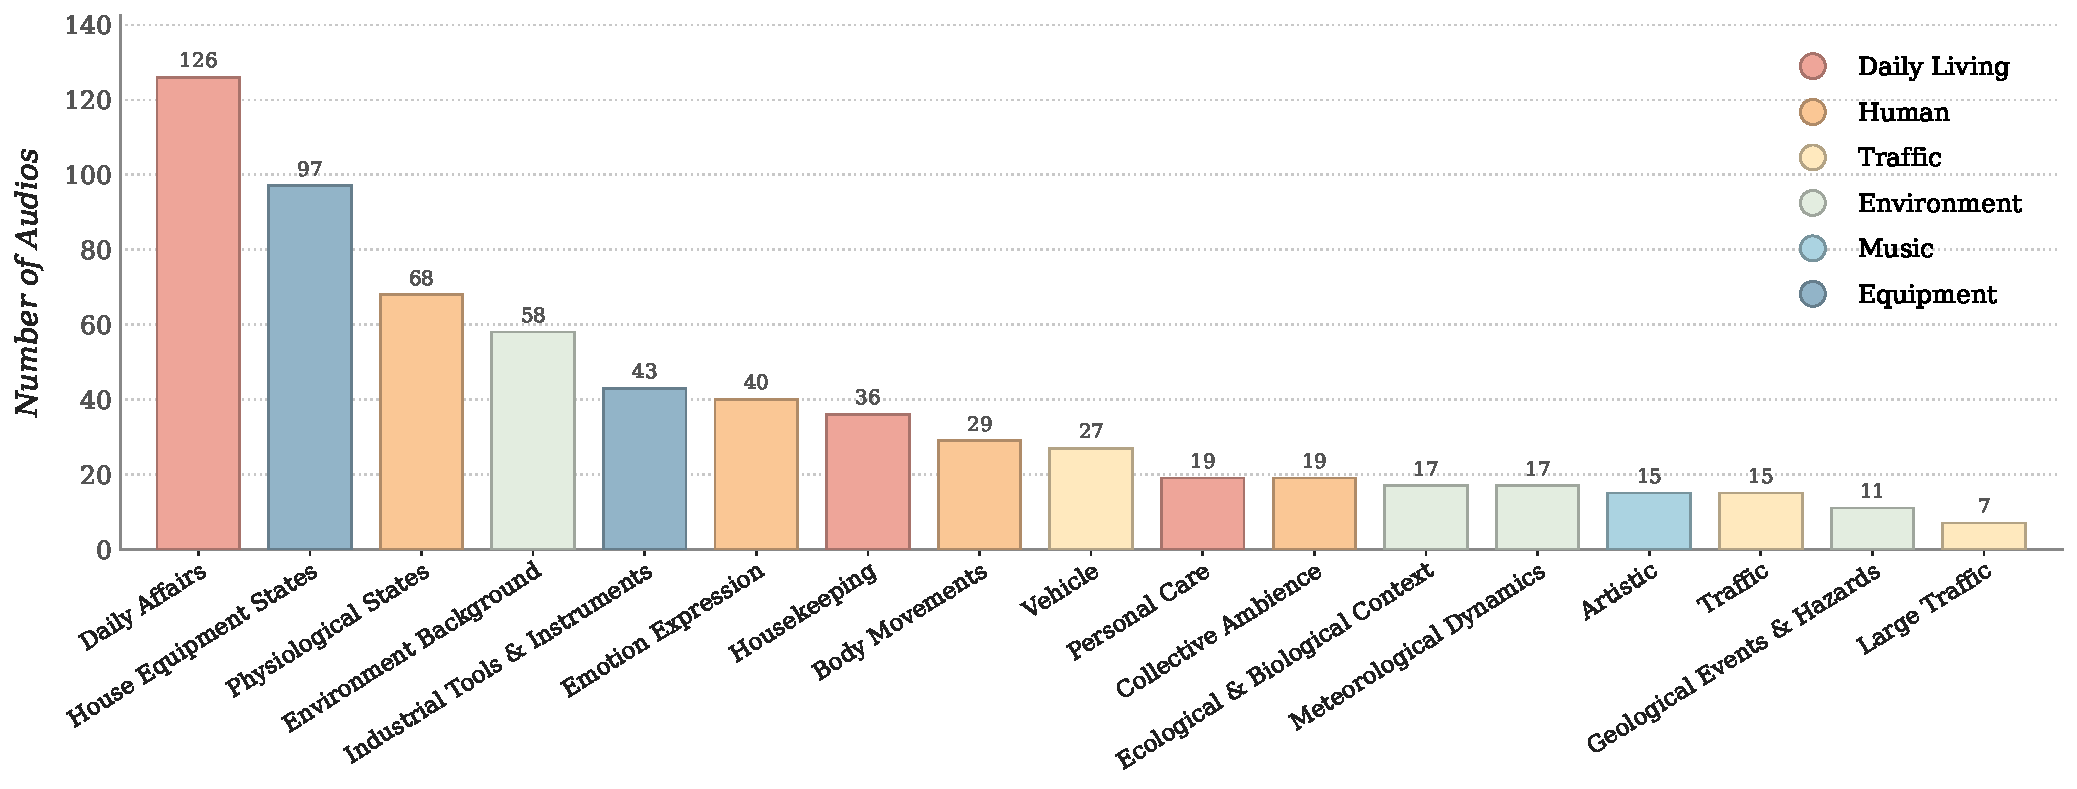
\includegraphics[width=1\linewidth]{fig/category_distribution.pdf}
    \caption{Enter Caption}
    \label{fig:placeholder}
\end{figure}
\paragraph{Taxonomy rationale.}
The macro-level taxonomy of ProactiveSound-Bench is designed to broadly cover acoustic scenarios that assistant devices may encounter in everyday life.
We construct it by progressively partitioning sounds according to how strongly they originate from the human body versus non-physiological sources.
First, we separate cues that arise \emph{directly from humans} from those that do not; the former are grouped into \textbf{Human Sound Signals}, emphasizing ``human-in-the-loop'' acoustics such as crying, breathing- and ingestion-related cues, salient emotional vocalizations, body-motion sounds, and crowd-like ambience---while excluding text-based user queries as task inputs.
Second, we include contexts that are strongly tied to human activity yet are not primarily human physiological productions: these typically correspond to object handling and domestic routines in living spaces, captured by \textbf{Daily Living Sounds} to characterize passive ``doing-things-at-home'' acoustics and their decision boundaries.
Third, we cover scenarios that are comparatively weakly tied to the human subject and are dominated by environmental processes or engineered systems: outdoor/natural dynamics are grouped under \textbf{Nature \& Environment}, electromechanical devices and tools under \textbf{Equipment}, and roadway/vehicle-dominated listening conditions under \textbf{Traffic}; together these cover most everyday ``environment--device--traffic'' sound regimes.
Finally, we add \textbf{Music}, which focuses on \emph{instrument-playing} related acoustic events and includes both nominally normal performances and severely out-of-tune corruptions caused by instrument damage.

\begin{table}[H]
  \centering
  \caption{Meso-level category definitions for ProactiveSound-Bench (conceptual scope only; exemplars are reported separately).}
  \label{tab_meso_definitions}
  \small
  \setlength{\tabcolsep}{6pt}
  \renewcommand{\arraystretch}{1.3} 
  \begin{tabular}{@{} 
      >{\raggedright\arraybackslash}p{3.05cm}
      >{\raggedright\arraybackslash}p{2.35cm}
      p{0.545\linewidth} @{}}
    \toprule
    \textbf{Meso subdomain} & \textbf{Macro domain} & \textbf{Definition} \\
    \midrule
    Body Movements      & Human & Characterizing acoustics associated with exercise and injury. \\
    
    
    Physiological states & Human & Auditory information associated with normal bodily functions or acute physiological stress. \\
    Emotion Expression   & Human & Significant affective vocalizations and expressive non-verbal signals. \\
    Collective Ambience  & Human & The dominant background environment in which a crowd participates in an activity. \\
    \midrule
    Personal Care       & Daily Living & Domestic self-care workflows in private living spaces. \\
    
    Daily Affairs       & Daily Living & Routine indoor micro-interactions with furniture, handheld objects and dynamic surfaces. \\
    
    Housekeeping        & Daily Living & Cleaning- and tidying-centric domestic workflows dominated by repetitive surface interactions and maintenance motions. \\
    \midrule
    House Equipment     & Equipment & Household electromechanical systems and appliances operation status. \\
    Industrial Tools    & Equipment & Tooling and industrial machinery acoustics associated with powered operation, and higher-energy mechanical transients. \\
    \midrule
    Vehicle             & Traffic & Focusing on the acoustic signals of vehicle mechanical systems. \\
    Traffic             & Traffic & Intermittent Warning Signals in Urban Road Soundscapes. \\
    Large Traffic       & Traffic & Mass-transit and heavy-vehicle dominated contexts characterized by periodic rail/bogie rhythm, large chassis resonance. \\
    \midrule
    Meteorologys        & Environment & Weather-driven airborne and precipitation acoustics spanning calm atmospheric textures to highly dynamic storm processes. \\
    Geological Hazards  & Environment & Impact sounds generated by terrain dynamics serve as indicators of slope instability, rockfalls, or geological movements. \\
    Ecological Context  & Environment & Biotic outdoor cues attributable to animals/plants/ecosystem activity. \\
    Social places       & Environment & Human-occupied ambient soundscapes in social/public spaces. \\
    \midrule
    Artistic            & Music       & Instrument-forward performance acoustics. \\
    \bottomrule
  \end{tabular}
\end{table}


\newpage
\section{Experiments Details}
\label{appendix:hyperparams}

Table~\ref{tab:hyperparams} reports all method-, data-, and
optimization-level hyperparameters held fixed across the four-stage
training recipe of \S\ref{appendix:streaming-training}. Method-level
constants ($c$, $\omega$, $\delta$, $\lambda$) follow the design choices
identified by the ablations in \S5.4; data-level constants
($\tau_{\text{wer}}$, $R$, SNR, role gains, Stage~4 mix probabilities)
follow the values introduced in \S\ref{appendix:curation}. Optimization
hyperparameters vary per stage to match each stage's data scale and
trainable-parameter footprint: the streaming SFT stage receives the
largest step budget, while the instruction-following stage uses the
lowest learning rate to preserve previously acquired capabilities. All
training is conducted in bf16 mixed precision with gradient checkpointing
and DeepSpeed ZeRO-2 sharding on $32\!\times\!\textsc{NVIDIA H100}$
$80$\,GB GPUs.

\begin{table}[H]
\centering
\caption{Configurations of parameters in Audio-Interaction.}
\label{tab:hyperparams}
\footnotesize
\setlength{\tabcolsep}{4pt}
\renewcommand{\arraystretch}{1.05}
\begin{tabular}{c|l|cccc}
\toprule
\textbf{Configurations} & \textbf{Parameters} & \multicolumn{4}{c}{\textbf{Values}} \\
\cmidrule(lr){3-6}
 &  & \textbf{Stage 1} & \textbf{Stage 2} & \textbf{Stage 3} & \textbf{Stage 4} \\
\midrule
\multirow{5}{*}{Streaming}
  & chunk size $c$                   & \multicolumn{4}{c}{$400$\,ms} \\
  & fade window $\omega$             & \multicolumn{4}{c}{$20$\,ms} \\
  & half-chunk align $\delta$        & \multicolumn{4}{c}{$200$\,ms} \\
  & dual-loss weight $\lambda$       & \multicolumn{4}{c}{$1.0$} \\
  & max stream length $L_{\max}$     & \multicolumn{4}{c}{$60$ chunks ($24$\,s)} \\
\midrule
\multirow{7}{*}{Data}
  & WER threshold $\tau_{\text{wer}}$ & \multicolumn{4}{c}{$0.10$} \\
  & ASR retries $R$                  & \multicolumn{4}{c}{$2$} \\
  & SNR distribution $P_{\text{snr}}$ & \multicolumn{4}{c}{$\mathcal{U}(5,\,20)$\,dB} \\
  & role gain (fg / bg / amb)        & \multicolumn{4}{c}{$0$ / $-6$ / $-12$\,dB} \\
  & history-review prob $p_{\text{hr}}$  & --- & --- & --- & $0.30$ \\
  & silent mix prob $p_{\text{sil}}$     & --- & --- & --- & $0.40$ \\
  & proactive mix prob $p_{\text{pro}}$  & --- & --- & --- & $0.30$ \\
\midrule
\multirow{11}{*}{Training}
  & trainable modules         & LM head + emb.       & adapter              & adapter + LM         & adapter + LM \\
  & batch size (per GPU)      & $8$                  & $8$                  & $4$                  & $2$ \\
  & gradient accum.\ steps    & $2$                  & $4$                  & $8$                  & $16$ \\
  & effective batch size      & $512$                & $1024$               & $1024$               & $1024$ \\
  & learning rate             & $1\!\times\!10^{-4}$ & $1\!\times\!10^{-4}$ & $5\!\times\!10^{-5}$ & $1\!\times\!10^{-5}$ \\
  & training steps            & $5$\,k               & $20$\,k              & $80$\,k              & $15$\,k \\
  & warmup ratio              & $0.03$               & $0.03$               & $0.03$               & $0.03$ \\
  & optimizer                 & \multicolumn{4}{c}{AdamW ($\beta_1\!=\!0.9$, $\beta_2\!=\!0.95$, $\varepsilon\!=\!10^{-8}$)} \\
  & scheduler                 & \multicolumn{4}{c}{Cosine decay with linear warmup} \\
  & weight decay              & \multicolumn{4}{c}{$0.01$} \\
  & max grad norm             & \multicolumn{4}{c}{$1.0$} \\
\midrule
\multirow{3}{*}{Hardware}
  & GPUs                      & \multicolumn{4}{c}{$32\!\times\!\textsc{NVIDIA H100}$ $80$\,GB} \\
  & precision \& sharding     & \multicolumn{4}{c}{bf16 mixed precision, DeepSpeed ZeRO-2} \\
  & total wall-clock time     & \multicolumn{4}{c}{$\sim 10$ days} \\
\bottomrule
\end{tabular}
\end{table}

\newpage
\section{Full Related Work}

\paragraph{Streaming Audio Models.}
In the streaming setting there is no single unified model. Instead,
each task is handled by a dedicated family of models that specializes
in a particular function. Representative examples include streaming
speech recognition~\citep{gao2022paramformer}, streaming speech
translation~\citep{seamless}, and full-duplex spoken
dialogue, which has become an important and rapidly developing
direction~\citep{lslm, miniomni2, silent, chronological}. DuplexSLA~\citep{duplexsla} further adds action to duplex models. Audio-interaction shares several
characteristics with this last class of models. It operates over
fixed-size audio chunks, ingesting acoustic frames sequentially and
deciding, on the basis of acoustic and semantic cues, whether and when
to intervene, as exemplified by Moshi~\citep{defossez2024moshi}. The decision
required in audio-interaction, however, is substantially more complex.
Beyond local acoustic and semantic signals, it must additionally
reason over full-audio understanding, environmental sounds,
paralinguistic information, and explicit user instructions, which
together make the intervention policy far richer than that of prior
streaming systems.

\paragraph{Audio Large Models.}
Audio large models represent a milestone toward a single unified model
that can perform general audio-based
tasks~\citep{chu2024qwen2, qwen25omni2025, diffa2, stepaudio2}. This
unification has given rise to a broad spectrum of capabilities, such
as speech understanding~\citep{sakshi2024mmau}, spoken-dialogue
understanding~\citep{mmsu}. Serving
as a general-purpose foundation, these models have been further
extended to a wide range of downstream tasks, including speech
recognition~\citep{xu2025fireredasr, seed-asr, qwen3-asr, megaasr},
emotion understanding~\citep{emotionthinker}, and audio
reasoning~\citep{afcot, thinkwith,
audiocog, audio-reasoner}. Despite this progress, current audio
large models remain exclusively offline. None of them offers a unified
model that can understand sound and the surrounding environment while
executing instructions in real time, and closing this gap is precisely
the motivation behind our work.

\paragraph{Streaming AI Systems.}
Artificial general intelligence cannot remain permanently behind the
screen. To be genuinely useful it must move to the foreground and
interact with humans directly, which motivates the development of
streaming models and systems. In the visual domain, this line of
research has produced continuous, online video understanding that
processes incoming frames as they arrive~\citep{chen2024videollm,
li2025videochat}. A more readily deployable alternative is the cascaded AI
system, such as proactive agents~\citep{proactive, proagent,
pask,needllm}, which place the text modality at the center of processing and
coordinate several specialized components. In contrast to these
designs, our work aims to open a new paradigm by realizing this
capability within a single end-to-end model.



\newpage
\section{Error Analyses}
\label{app:analysis}

\label{app:analysis:err:breakdown}
\begin{itemize}[leftmargin=0.5em,label=\textbullet,itemsep=0.35em,topsep=0.35em]
    \item \textbf{LibriSpeech(ASR).}
  
  On the LibriSpeech  error analysis of the 98 non‑empty and non‑crash predictions identifies four primary error categories. Local Token Deviation—grouping phonetically or orthographically motivated substitutions together with minor insertions and deletions—constitutes the largest error class, accounting for 60.2\% of all analyzed errors. Rare‑Word \& Long‑Utterance Degradation forms the second major category (21.4\%), characterized by the misrecognition of named entities and structural breakdown in syntactically complex sentences; literary character names and extended utterances prove particularly challenging. Function Word Bias (14.3\%) and Decoding Loop phenomena (4.1\%) appear at lower frequencies—the former arising from language model preferences for certain function words, and the latter manifested as phrase‑level repetition. Overall, these error patterns underscore targeted opportunities for improvement, while the model's strong baseline accuracy remains competitive with other approaches of comparable scale. 
  
    \item \textbf{CoVoST2(Speech-to-Text Translation).}
    In this error analysis, we examined the low-BLEU translations (BLEU < 20) produced by our S2TT model on the CoVoST2 English-to-Chinese test set. We categorized the errors into two main types. Semantic hallucinations, where the model generates a translation completely unrelated to the source audio, dominate the low-score set, accounting for 82\% of the cases. The remaining 18\% are incomplete or mixed-language outputs that contain untranslated English fragments, garbled symbols, or broken phrases, failing to form a coherent Chinese sentence. 

    Then,we conduct an error analysis on the lowest-BLEU  sentences in the zh→en CoVoST2 subset. Low-score cases fall into two dominant categories:  off-topic or hallucinated translations likely caused by severe recognition/misalignment failures, accounting for 75.5\% of errors;  and omissions or uncontrolled paraphrasing that preserve partial meaning but break n-gram overlap, accounting for 24.5\%. 

    \item \textbf{MMAU.(Audio Understanding)}
    The error analysis on our model's MMAU results uncovers two primary failure categories. Approximately 20\% arise from generation collapse, characterized by unparseable outputs that prevent any valid assessment. The remaining  represent genuine recognition or reasoning errors, where the model confused acoustically similar sources, misclassified speaker attributes like age or gender, or selected an incorrect category despite partially correct reasoning.

    \item \textbf{SpokenQA (Llama Questions \& Web Questions).}
    
  After excluding empty predictions (35 instances) and correct responses that were erroneously flagged as errors due to overly strict evaluation formatting, LlamaQA’s valid predictions contained a total of 37 actual model errors. These errors can be categorized into three types: Factual Hallucinations (56.8\%) were the most prominent, manifesting as the fabrication of non-existent names of people, places, or events, accompanied by fluent descriptions; Temporal and Quantitative Errors (16.2\%) involved providing incorrect specific figures or values in response to questions requiring precise numerical data; Irrelevant or Generalized Responses (27\%) substituted direct answers with poetic, vacuous, or evasive language; 

  Overall, the errors observed on the WebQuestions dataset can be categorized into three main types.
  Factual hallucinations constitute the largest share—approximately 71\%—referring to instances where the model fabricates factual content out of thin air that appears plausible yet is entirely unrelated to the correct answer, lacking any external knowledge support. Irrelevant or generalized responses account for roughly 15\%; this occurs when the output fails to provide the direct information requested by the query, instead offering roundabout replies characterized by hollow, flippant, or evasive language. Errors regarding time and quantity make up approximately 15\%, reflecting the model's tendency to provide incorrect specific values when addressing questions involving particular years, dates, time zones, or numerical figures.
   

  

    \item \textbf{VoiceBench (AlpacaEval-full \& SD-QA).}
  On VoiceBench's Alpaca-Eval subset, We categorize these low score samples into three types. (1) Hallucination (53.5\%): the model generates factually incorrect statements that contradict established knowledge, including fabricated entities, misattributed events, or erroneous numbers. (2) Irrelevant response or inappropriate refusal (46.4\%): the model produces content unrelated to the prompt or rejects a harmless request, often due to keyword misinterpretation or over-triggered safety filters. 
  
  The  incorrect answers in the SD‑QA subset exhibit three primary failure modes. Factual hallucination accounts for roughly 63\% of the errors, where the model confidently generates false details . Irrelevant or miscomprehending responses constitute about 24\%, where the question is misheard and an off‑topic answer is given . The remaining 13\% are over‑refusals, in which innocuous factual queries are wrongly rejected as sensitive .


    \item \textbf{ProactiveSound-Bench.}
    Among errors. False positives(59.8\%) were dominated by overreactions to benign daily sounds such as tearing paper, appliance noises, drinking, or sighs, generating unnecessary alerts . Conversely, false negatives(40.2\%) clustered in safety‑critical domains like traffic alarms, natural hazard.

\end{itemize}



% \appendix
% \newpage

% \section{Training details}
% \paragraph{Implementation Details.}
% Mini-Omni~3 is built on Qwen2.5-Omni-3B and trained on StreamAudio-2M for $4$ epochs based on $8$ NVIDIA L40s GPUs. The optimizer is AdamW with a learning rate of $2\!\times\!10^{-4}$, cosine schedule. The encoder frame rate is set to $0.04$~s per audio token, and a streaming decision is made every $0.4$~s ($10$ tokens). More implementation details are listed in Appendix~\ref{app:impl}.



% \section{Technical appendices and supplementary material}
% Technical appendices with additional results, figures, graphs, and proofs may be submitted with the paper submission before the full submission deadline (see above). You can upload a ZIP file for videos or code, but do not upload a separate PDF file for the appendix. There is no page limit for the technical appendices. 

% Note: Think of the appendix as ``optional reading'' for reviewers. The paper must be able to stand alone without the appendix; for example, adding critical experiments that support the main claims to an appendix is inappropriate. 





\newpage
\bibliographystyle{plainnat}



\end{document}